% Arquivo LaTeX de exemplo de dissertação/tese a ser apresentada à CPG do IME-USP
%
% Criação: Jesús P. Mena-Chalco
% Revisão: Fabio Kon e Paulo Feofiloff
% Adaptação para UTF8, biblatex e outras melhorias: Nelson Lago
%
% Except where otherwise indicated, these files are distributed under
% the MIT Licence. The example text, which includes the tutorial and
% examples as well as the explanatory comments in the source, are
% available under the Creative Commons Attribution International
% Licence, v4.0 (CC-BY 4.0) - https://creativecommons.org/licenses/by/4.0/


%%%%%%%%%%%%%%%%%%%%%%%%%%%%%%%%%%%%%%%%%%%%%%%%%%%%%%%%%%%%%%%%%%%%%%%%%%%%%%%%
%%%%%%%%%%%%%%%%%%%%%%%%%%%%%%% PREÂMBULO LaTeX %%%%%%%%%%%%%%%%%%%%%%%%%%%%%%%%
%%%%%%%%%%%%%%%%%%%%%%%%%%%%%%%%%%%%%%%%%%%%%%%%%%%%%%%%%%%%%%%%%%%%%%%%%%%%%%%%

% "Book" tem capítulos (e partes, mas normalmente não usamos) e, se o documento
% é frente-e-verso, cada capítulo começa em uma página de numeração ímpar.
% Report é similar, mas cada capítulo começa em uma nova página, par ou ímpar.
% É possível mudar esse comportamento com a opção "openany". Observe que você
% pode adaptar este modelo para escrever artigos, mudando a classe do
% documento de "book" para "article" ou a classe de algum periódico específico.
% No entanto, o arquivo "artigo.tex" é um ponto de partida melhor: ele é
% similar a este, mas já inclui as mudanças necessárias para a classe article.
%
% A opção frente-e-verso aqui significa, por exemplo, que as margens das páginas
% ímpares e pares são diferentes ou que números de página aparecem à direita
% ou à esquerda alternadamente. Nada impede que você crie um documento "só
% frente" e, ao imprimir, faça a impressão frente-e-verso.
%
% Aqui também definimos a língua padrão do documento e línguas adicionais. A
% classe em si não usa essa informação mas, passando as opções de língua aqui,
% elas são repassadas para todas as packages, e diversas packages mudam
% seu comportamento em função da língua (em especial, babel/polyglossia).
% A última língua da lista é a língua padrão do documento.
%\documentclass[12pt,twoside,brazil,english]{book}
\documentclass[12pt,twoside,english,brazil]{book}

% Com papel tamanho A4, queremos estas margens:
%
% topo: 32mm
% pé: 28mm
% esquerda/interna: 24mm
% direita/externa: 34mm
%
% Para isso, definimos os tamanhos do texto, do cabeçalho e do rodapé,
% e deixamos a package geometry calcular os demais valores. Assim,
% obtemos o mesmo resultado impresso, mas com margens diferentes, se
% o tamanho do papel for diferente.

\usepackage[a4paper]{geometry}

\geometry{
  %top=32mm,
  %bottom=28mm,
  %left=24mm,
  %right=34mm,
  textwidth=152mm, % 210-24-34
  textheight=237mm, % 297-32-28
  vmarginratio=8:7, % 32:28
  hmarginratio=12:17, % 24:34
  % Com geometry, esta medida não é tão relevante; basta garantir que ela
  % seja menor que "top" e que o texto do cabeçalho caiba nela.
  headheight=25.4mm,
  % distância entre o início do texto principal e a base do cabeçalho;
  % ou seja, o cabeçalho "invade" a margem superior nessa medida. Essa
  % é a medida que determina a posição do cabeçalho
  headsep=11mm,
  footskip=10mm,
  marginpar=20mm,
  marginparsep=5mm,
}

% Vários pacotes e opções de configuração genéricos; para personalizar o
% resultado, modifique estes arquivos.
%%%%%%%%%%%%%%%%%%%%%%%%%%%%%%%%%%%%%%%%%%%%%%%%%%%%%%%%%%%%%%%%%%%%%%%%%%%%%%%%
%%%%%%%%%%%%%%%%%%%%%%% CONFIGURAÇÕES E PACOTES BÁSICOS %%%%%%%%%%%%%%%%%%%%%%%%
%%%%%%%%%%%%%%%%%%%%%%%%%%%%%%%%%%%%%%%%%%%%%%%%%%%%%%%%%%%%%%%%%%%%%%%%%%%%%%%%

% Vários comandos auxiliares para o desenvolvimento de packages e classes;
% aqui, usamos em alguns comandos de formatação e condicionais.
\usepackage{etoolbox}
\usepackage{xstring}
\usepackage{xparse}
\usepackage{regexpatch}
% Esta não está em uso mas pode ser útil.
%\usepackage{ltxcmds}

% Esta package permite detectar XeTeX, LuaTeX e pdfTeX, mas pode não estar
% disponível em todas as instalações de TeX.
%\usepackage{iftex}
% Por conta disso, usaremos estas (que não detectam pdfTeX):
\usepackage{ifxetex}
\usepackage{ifluatex}

\newbool{unicodeengine}
\ifboolexpr{bool{xetex} or bool{luatex}}
  {\booltrue{unicodeengine}}
  {\boolfalse{unicodeengine}}

% Detecta se estamos produzindo um arquivo PDF ou DVI (lembrando que tanto
% pdfTeX quanto LuaTeX podem gerar ambos)
\usepackage{ifpdf}

% Algumas packages "padrão" da AMS, que são praticamente  obrigatórias.
% Algumas delas devem ser carregadas antes de unicode-math ou das
% definições das fontes do documento.
\usepackage{amssymb}
\usepackage{amsthm}
\usepackage{amsmath}
\usepackage{mathtools}

\ifunicodeengine
  % Não é preciso carregar fontenc e inputenc com LuaTeX e XeTeX!
  \usepackage{fontspec}
  \usepackage{unicode-math}
\else
  % "fontenc" é um parâmetro interno do LaTeX. Com pdfLaTeX, o fontenc
  % default é OT1, mas ele tem algumas limitações; a mais importante é
  % que, com ele, palavras acentuadas não podem ser hifenizadas. Por
  % conta disso, quase todos os documentos LaTeX utilizam o fontenc T1.
  % A escolha do fontenc tem consequências para as fontes que podem ser
  % usadas no documento; hoje em dia T1 tem mais opções de qualidade,
  % então não se perde nada.
  \usepackage[T1]{fontenc}
  \usepackage[utf8]{inputenc}
  \usepackage{fontaxes}
\fi

% Internacionalização dos nomes das seções ("chapter" X "capítulo" etc.),
% hifenização e outras convenções tipográficas. babel deve ser um dos
% primeiros pacotes carregados. É possível passar a língua do documento
% como parâmetro aqui, mas já fizemos isso ao carregar a classe, no início
% do documento.
\usepackage{babel}

% É possível personalizar as palavras-chave que babel utiliza, por exemplo:
%\addto\extrasbrazil{\renewcommand{\chaptername}{Chap.}}
% Com BibTeX, isso vale também para a bibliografia; com BibLaTeX, é melhor
% usar o comando "DefineBibliographyStrings".

% Para línguas baseadas no alfabeto latino, como o inglês e o português,
% o pacote babel funciona muito bem, mas com outros alfabetos ele às vezes
% falha. Por conta disso, o pacote polyglossia foi criado para substituí-lo.
% polyglossia só funciona com LuaTeX e XeTeX; como babel também funciona com
% esses sistemas, provavelmente não há razão para usar polyglossia, mas é
% possível que no futuro esse pacote se torne o padrão.
%\usepackage{polyglossia}
%\setdefaultlanguage{brazil}
%\setotherlanguage{english}

% Alguns pacotes (espeficicamente, tikz) usam, além de babel, este pacote
% como auxiliar para a tradução de palavras-chave, como os meses do ano.
\usepackage{translator}

% microajustes no tamanho das letras, espaçamento etc. para melhorar
% a qualidade visual do resultado. LaTeX tradicional não dá suporte a
% nenhum tipo de microajuste; pdfLaTeX dá suporte a todos. LuaLaTeX
% e XeLaTeX dão suporte a alguns:
%
% * expansion não funciona com XeLaTeX
% * tracking não funciona com XeLaTeX; é possível obter o mesmo resultado
%   com a opção "LetterSpace" do pacote fontspec, mas a configuração é
%   totalmente manual. Por padrão, aumenta o afastamento entre caracteres
%   nas fontes "small caps"; o resultado não se presta ao uso na
%   bibliografia ou citações, então melhor desabilitar.
% * kerning e spacing só funcionam com pdfLaTex; ambas são funções
%   consideradas experimentais e nem sempre produzem resultados vantajosos.

\newcommand\microtypeopts{
  protrusion=true,
  tracking=false,
  kerning=false,
  spacing=false
}

% TeXLive 2018 inclui a versão 2.7a da package microtype e a versão
% 1.07 de luatex. Essa combinação faz aparecer um bug:
% https://tex.stackexchange.com/questions/476740/microtype-error-with-lualatex-attempt-to-call-field-warning-a-nil-value
% Aqui, aplicamos a solução sugerida, que não tem "contra-indicações".
\ifluatex
  \usepackage{luatexbase}
\fi

\ifxetex
  \usepackage[expansion=false,\microtypeopts]{microtype}
\else
  \usepackage[expansion=true,\microtypeopts]{microtype}
\fi

% Alguns "truques" (sujos?) para minimizar over/underfull boxes.
%
% Para fazer um texto justificado, é preciso modificar o tamanho dos espaços
% em cada linha para mais ou para menos em relação ao seu tamanho ideal. Para
% escolher as quebras de linha, TeX vai percorrendo o texto procurando lugares
% possíveis para quebrar as linhas considerando essa flexibilidade mas dentro
% de um certo limite mínimo/máximo. Nesse processo, ele associa a cada possível
% linha o valor badness, que é o nível de distorção do tamanho dos espaços
% daquela linha em relação ao ideal, e ignora opções que tenham badness muito
% grande (esse limite é dado por \tolerance). Depois de encontradas todas as
% possíveis quebras de linha e a badness de cada uma, TeX calcula as penalties
% e demerits de cada possibilidade e escolhe a solução que minimiza o demerit
% total do parágrafo.
%
% Para cada fonte, o espaço em TeX tem um tamanho ideal, um tamanho mínimo e um
% tamanho máximo. TeX nunca reduz um espaço para menos que o mínimo da fonte,
% mas pode aumentá-lo para mais que o máximo. Se os espaços de uma linha ficam
% com o tamanho ideal, a badness da linha é 0; se o tamanho é
% reduzido/aumentado 50% do mínimo/máximo, a badness da linha é 12; se o
% tamanho é reduzido/aumentado para o mínimo/máximo, a badness é 100. Se esse
% aumento for de 30% além do máximo, a badness da linha é 200; se for de 45%
% além do máximo, a badness é 300; se for de 60% além do máximo, a badness é
% 400; se for de 100% além do máximo, a badness é 800.
%
% A \tolerance default é 200; aumentar para, digamos, 300 ou 400, permite que
% TeX escolha parágrafos com maior variação no espaçamento. No entanto, no
% cálculo de demerits, a badness de cada linha é elevada ao quadrado, então TeX
% geralmente prefere escolher outras opções no lugar de uma linha ruim. Por
% exemplo, órfãs/viúvas têm demerit de 22.500 e dois hífens seguidos têm
% demerit de 10.000 e, portanto, não é surpreendente que a maioria dos
% parágrafos tenha demerits abaixo de 40.000, quase todos abaixo de 100.000 e
% praticamente nenhum acima de 1.000.000. Isso significa que, para a grande
% maioria dos parágrafos, aumentar \tolerance não faz diferença: uma linha com
% badness 400 (correspondendo a demerit de 160.000) nunca será efetivamente
% escolhida se houver qualquer outra opção com badness menor. Também fica claro
% que não há muita diferença real entre definir \tolerance como 800 ou 9.999.
%
% O problema muda de figura se TeX não consegue encontrar uma solução. Isso
% pode acontecer em dois casos: (1) o parágrafo tem ao menos uma linha que não
% pode ser quebrada com badness < 10.000 e (2) o parágrafo tem ao menos uma
% linha que não pode ser quebrada com badness < tolerance (mas essa badness é
% menor que 10.000).
%
% No primeiro caso, se houver várias possibilidades de linhas que não podem ser
% quebradas, TeX não vai ser capaz de compará-las e escolher a melhor: todas
% têm a badness máxima (10.000) e, portanto, a que gerar menos deméritos no
% restante do parágrafo será a escolhida. Na realidade, no entanto, essas
% linhas *não* são igualmente ruins entre si, o que pode levar TeX a fazer uma
% má escolha. Para evitar isso, TeX tenta novamente aplicando
% \emergencystretch, que "faz de conta" que o tamanho máximo ideal dos espaços
% da linha é maior que o definido na fonte. Isso reduz a badness de todas as
% linhas, o que soa parecido com aumentar \tolerance. Há três diferenças, no
% entanto: (1) essa mudança só afeta os parágrafos que falharam; (2) soluções
% que originalmente teriam badness = 10.000 (e, portanto, seriam vistas como
% equivalentes) podem ser avaliadas e comparadas entre si; e (3) como a badness
% de todas as linhas diminui, a possibilidade de outras linhas que
% originalmente tinham badness alta serem escolhidas aumenta. Esse último ponto
% significa que \emergencystretch pode fazer TeX escolher linhas mais
% espaçadas, fazendo o espaçamento do parágrafo inteiro aumentar e, portanto,
% tornando o resultado mais homogêneo mesmo com uma linha particularmente ruim.
%
% É esse último ponto que justifica o uso de \emergencystretch no segundo caso
% também: apenas aumentar a tolerância, nesse caso, poderia levar TeX a
% diagramar uma linha ruim em meio a um parágrafo bom, enquanto
% \emergencystretch pode fazer TeX aumentar o espaçamento de maneira geral no
% parágrafo, minimizando o contraste da linha problemática com as demais.
% Colocando a questão de outra maneira, aumentar \tolerance para lidar com
% esses parágrafos problemáticos pode fazê-los ter uma linha especialmente
% ruim, enquanto \emergencystretch pode dividir o erro entre várias linhas.
% Assim, definir \tolerance em torno de 800 parece razoável: no caso geral,
% não há diferença e, se um desses casos difíceis não pode ser resolvido com
% uma linha de badness até 800, \emergencystretch deve ser capaz de gerar um
% resultado igual ou melhor.
%
% Penalties & demerits: https://tex.stackexchange.com/a/51264
% Definições (fussy, sloppy etc.): https://tex.stackexchange.com/a/241355
% Mais definições (hfuzz, hbadness etc.): https://tex.stackexchange.com/a/50850
% Donald Arseneau defendendo o uso de \sloppy: https://groups.google.com/d/msg/comp.text.tex/Dhf0xxuQ66E/QTZ7aLYrdQUJ
% Artigo detalhado sobre \emergencystretch: https://www.tug.org/TUGboat/tb38-1/tb118wermuth.pdf
% Esse artigo me leva a crer que algo em torno de 1.5em é suficiente

\tolerance=800
\hyphenpenalty=100 % Default 50; se o texto é em 2 colunas, 50 é melhor
\setlength{\emergencystretch}{2.5em}

% Não gera warnings para Overfull menor que 0.5pt
\hfuzz=.5pt
\vfuzz\hfuzz

% Não gera warnings para Underfull com badness < 1000
\hbadness=1000
\vbadness=1000

% LaTeX às vezes coloca notas de rodapé logo após o final do texto da
% página ao invés de no final da página; este pacote evita isso.
\usepackage[bottom]{footmisc}

% Se uma página está vazia, não imprime número de página ou cabeçalho
\usepackage{emptypage}

% Espaçamento entre linhas configurável (\singlespacing, \onehalfspacing etc.)
\usepackage{setspace}

% Carrega nomes de cores disponíveis (podem ser usados com hyperref e listings)
\usepackage[hyperref,svgnames,x11names,table]{xcolor}

% LaTeX define os comandos "MakeUppercase" e "MakeLowercase", mas eles têm
% algumas limitações; esta package define os comandos MakeTextUppercase e
% MakeTextLowercase que resolvem isso.
\usepackage{textcase}

% Normalmente, LaTeX faz o final da página terminar sempre no mesmo lugar
% (exceto no final dos capítulos). Esse padrão pode ser ativado explicitamente
% com o comando "\flushbottom". Mas se, por alguma razão, o volume de texto na
% página é "pequeno", essa página vai ter espaços verticais artificialmente
% grandes. Uma solução para esse problema é modificar o padrão para
% "\raggedbottom"; isso permite que as páginas terminem em lugares diferentes.
% Outra opção é corrigir manualmente cada página problemática, por exemplo
% com o comando "\enlargethispage".
%\raggedbottom

% Por padrão, LaTeX coloca uma espaço aumentado após sinais de pontuação;
% Isso não é tão bom quanto alguns TeX-eiros defendem :) .
% Esta opção desabilita isso e, consequentemente, evita problemas com
% "id est" (i.e.) e "exempli gratia" (e.g.)
\frenchspacing

% LaTeX procura por arquivos adicionais no diretório atual e nos diretórios
% padrão do sistema. Assim, é preciso usar caminhos relativos para incluir
% arquivos de subdiretórios: "\input{diretorio/arquivo}". No entanto, há
% duas limitações:
%
% 1. É necessário dizer "\input{diretorio/arquivo} mesmo quando o arquivo
%    que contém esse comando já está dentro do subdiretório.
%
% 2. Isso não deve ser usado para packages ("\usepackage{diretorio/package}"),
%    embora na prática funcione.
%
% O modo recomendado de resolver esses problemas é modificando o arquivo
% texmf.cnf ou a variável de ambiente TEXINPUTS ou colocando os arquivos
% compartilhados na árvore TEXMF (geralmente, no diretório texmf dentro do
% diretório do usuário), o que é um tanto complicado para usuários menos
% experientes.
%
% O primeiro problema pode ser solucionado também com a package import,
% mas não há muita vantagem pois é preciso usar outro comando no lugar de
% "\input". O segundo problema é mais importante, pois torna muito difícil
% colocar packages adicionais em um diretório separado. Para contorná-lo,
% vamos usar um truque que é suficiente para nossa necessidade, embora
% *não* seja normalmente recomendado.
%\usepackage{import}

\newcommand\dowithsubdir[2]{
    \csletcs{@oldinput@path}{input@path}
    \csappto{input@path}{{#1}}
    #2
    \csletcs{input@path}{@oldinput@path}
}

%%%%%%%%%%%%%%%%%%%%%%%%%%%%%%%%%%%%%%%%%%%%%%%%%%%%%%%%%%%%%%%%%%%%%%%%%%%%%%%%
%%%%%%%%%%%%%%%%%%%%%%%%%%%%%%%%%%% FONTE %%%%%%%%%%%%%%%%%%%%%%%%%%%%%%%%%%%%%%
%%%%%%%%%%%%%%%%%%%%%%%%%%%%%%%%%%%%%%%%%%%%%%%%%%%%%%%%%%%%%%%%%%%%%%%%%%%%%%%%

% LaTeX normalmente usa quatro tipos de fonte:
%
% * uma fonte serifada, para o corpo do texto;
% * uma fonte com design similar à anterior para modo matemático;
% * uma fonte sem serifa, para títulos ou "entidades". Por exemplo, "a classe
%   \textsf{TimeManager} é responsável..." ou "chamamos \textsf{primos} os
%   números que...". Observe que em quase todos os casos desse tipo é mais
%   adequado usar negrito ou itálico;
% * uma fonte "teletype", para trechos de programas.
%
% A escolha de uma família de fontes para o documento normalmente é feita
% carregando uma package específica que, em geral, seleciona as quatro fontes
% de uma vez. Com LuaLaTeX/XeLaTeX, é possível usar os comandos da package
% fontspec para controlar em detalhes as fontes do documento.

% LaTeX usa por default a família de fontes "Computer Modern". Essas fontes
% precisaram ser re-criadas diversas vezes em formatos diferentes, então há
% diversas variantes dela. Com o fontenc OT1 (default "ruim" do LaTeX), a
% versão usada é a BlueSky Computer Modern, que é de boa qualidade, mas com
% os problemas do OT1. Com fontenc T1 (padrão deste modelo quando usamos
% pdfLaTeX e recomendado), o LaTeX usa o conjunto "cm-super". Com fontspec
% (ou seja, com LuaLaTeX e XeLaTeX), LaTeX utiliza a versão "Latin Modern".
% Ao longo do tempo, versões diferentes dessas fontes foram recomendadas
% como "a melhor"; atualmente, a melhor opção para usar a família Computer
% Modern é a versão "Latin Modern".

\ifunicodeengine
    % Com LuaLaTex e XeLaTeX, Latin Modern é a fonte padrão. Existem
    % diversas packages e "truques" para melhorar alguns aspectos de
    % Latin Modern, mas eles foram feitos para pdflatex (veja o "else"
    % logo abaixo). Assim, se você pretende usar Latin Modern como a
    % fonte padrão do documento, é melhor usar pdfLaTeX. Deve ser
    % possível implementar essas melhorias com fontspec também, mas
    % este modelo não faz isso, apenas ativamos Small Caps aqui.

    \ifluatex
      % Com LuaTeX, basta indicar o nome de cada fonte; para descobrir
      % o nome "certo", use o comando "otfinfo -i" e veja os itens
      % "preferred family" e "full name"
      \setmainfont{Latin Modern Roman}[
        SmallCapsFont = {LMRomanCaps10-Regular},
        ItalicFeatures = {
          SmallCapsFont = {LMRomanCaps10-Oblique},
        },
        SlantedFont = {LMRomanSlant10-Regular},
        SlantedFeatures = {
          SmallCapsFont = {LMRomanCaps10-Oblique},
          BoldFont = {LMRomanSlant10-Bold}
        },
      ]
    \fi

    \ifxetex
      % Com XeTeX, é preciso informar o nome do arquivo de cada fonte.
      \setmainfont{lmroman10-regular.otf}[
        SmallCapsFont = {lmromancaps10-regular.otf},
        ItalicFeatures = {
          SmallCapsFont = {lmromancaps10-oblique.otf},
        },
        SlantedFont = {lmromanslant10-regular.otf},
        SlantedFeatures = {
          SmallCapsFont = {lmromancaps10-oblique.otf},
          BoldFont = {lmromanslant10-bold.otf}
        },
      ]
    \fi

\else
    % Usando pdfLaTeX

    % Ativa Latin Modern como a fonte padrão.
    \usepackage{lmodern}

    % Alguns truques para melhorar a aparência das fontes Latin Modern;
    % eles não funcionam com LuaLaTeX e XeLaTeX.

    % Latin Modern não tem fontes bold + Small Caps, mas cm-super sim;
    % assim, vamos ativar o suporte às fontes cm-super (sem ativá-las
    % como a fonte padrão do documento) e configurar substituições
    % automáticas para que a fonte Latin Modern seja substituída por
    % cm-super quando o texto for bold + Small Caps.
    \usepackage{fix-cm}

    % Com Latin Modern, é preciso incluir substituições para o encoding TS1
    % também por conta dos números oldstyle, porque para inclui-los nas fontes
    % computer modern foi feita uma hack: os dígitos são declarados como sendo
    % os números itálicos da fonte matemática e, portanto, estão no encoding TS1.
    %
    % Primeiro forçamos o LaTeX a carregar a fonte Latin Modern (ou seja, ler
    % o arquivo que inclui "DeclareFontFamily") e, a seguir, definimos a
    % substituição
    \fontencoding{TS1}\fontfamily{lmr}\selectfont
    \DeclareFontShape{TS1}{lmr}{b}{sc}{<->ssub * cmr/bx/n}{}
    \DeclareFontShape{TS1}{lmr}{bx}{sc}{<->ssub * cmr/bx/n}{}

    \fontencoding{T1}\fontfamily{lmr}\selectfont
    \DeclareFontShape{T1}{lmr}{b}{sc}{<->ssub * cmr/bx/sc}{}
    \DeclareFontShape{T1}{lmr}{bx}{sc}{<->ssub * cmr/bx/sc}{}

    % Latin Modern não tem "small caps + itálico", mas tem "small caps + slanted";
    % vamos definir mais uma substituição aqui.
    \fontencoding{T1}\fontfamily{lmr}\selectfont % já feito acima, mas tudo bem
    \DeclareFontShape{T1}{lmr}{m}{scit}{<->ssub * lmr/m/scsl}{}
    \DeclareFontShape{T1}{lmr}{bx}{scit}{<->ssub * lmr/bx/scsl}{}

    % Se fizermos mudanças manuais na fonte Latin Modern, estes comandos podem
    % vir a ser úteis
    %\newcommand\lmodern{%
    %  \renewcommand{\oldstylenums}[1]{{\fontencoding{TS1}\selectfont ##1}}%
    %  \fontfamily{lmr}\selectfont%
    %}
    %
    %\DeclareRobustCommand\textlmodern[1]{%
    %  {\lmodern #1}%
    %}
\fi

% Algumas packages mais novas que tratam de fontes funcionam corretamente
% tanto em LuaLaTeX/XeLaTeX quanto em pdfLaTeX, mas várias funcionam
% apenas em pdfLaTeX. Nesse caso, em LuaLaTeX/XeLaTeX é preciso usar os
% comandos de fontspec, como exemplificado mais abaixo.

% É possível mudar apenas uma das fontes. Em particular, a fonte
% teletype da família Computer Modern foi criada para simular
% as impressoras dos anos 1970/1980. Sendo assim, ela é uma fonte (1)
% com serifas e (2) de espaçamento fixo. Hoje em dia, é mais comum usar
% fontes sem serifa para representar código-fonte. Além disso, ao imprimir,
% é comum adotar fontes que não são de espaçamento fixo para fazer caber
% mais caracteres em uma linha de texto. Algumas opções de fontes para
% esse fim:
%\usepackage{newtxtt}
%\usepackage{DejaVuSansMono}
\ifunicodeengine
  \setmonofont{inconsolatan}
\else
  \usepackage[narrow]{inconsolata}
\fi

% Ao invés da família Computer Modern, é possível usar outras como padrão.
% Uma ótima opção é a libertine, similar (mas não igual) à Times mas com
% suporte a Small Caps e outras qualidades. A fonte teletype da família
% é serifada, então é melhor definir outra; a opção "mono=false" faz
% o pacote não carregar sua própria fonte, mantendo a escolha anterior.
% Versões mais novas de LaTeX oferecem um fork desta fonte, libertinus.
% As packages libertine/libertinus funcionam corretamente com pdfLaTeX,
% LuaLaTeX e XeLaTeX.
\makeatletter
\IfFileExists{libertinus.sty}
    {
      \usepackage[mono=false]{libertinus}
      % Com LuaLaTeX/XeLaTeX, Libertinus configura também
      % a fonte matemática; aqui só precisamos corrigir \mathit
      \ifunicodeengine
        \ifluatex
          \setmathfontface\mathit{Libertinus Serif Italic}
        \fi
        \ifxetex
          % O nome de arquivo da fonte mudou na versão 2019-04-04
          \@ifpackagelater{libertinus-otf}{2019/04/03}
              {\setmathfontface\mathit{LibertinusSerif-Italic.otf}}
              {\setmathfontface\mathit{libertinusserif-italic.otf}}
        \fi
      \fi
    }
    {
      % Libertinus não está disponível; vamos usar libertine
      \usepackage[mono=false]{libertine}

      % Com Libertine, é preciso modificar também a fonte
      % matemática, além de \mathit
      \ifunicodeengine
        \ifluatex
	  \setmathfont{Libertinus Math}
          \setmathfontface\mathit{Linux Libertine O Italic}
        \fi

        \ifxetex
          \setmathfont{libertinusmath-regular.otf}
          \setmathfontface\mathit{LinLibertine_RI.otf}
        \fi
      \fi
    }
\makeatother

\ifunicodeengine
  \relax
\else
  % A família libertine por padrão não define uma fonte matemática
  % específica para pdfLaTeX; uma opção que funciona bem com ela:
  %\usepackage[libertine]{newtxmath}
  % Outra, provavelmente melhor:
  \usepackage{libertinust1math}
\fi

% Ativa apenas a fonte biolinum, que é a fonte sem serifa da família.
%\usepackage{biolinum}

% Também é possível usar a Times como padrão; nesse caso, a fonte sem serifa
% é a Helvetica. Mas provavelmente libertine é uma opção melhor.
%\usepackage[helvratio=0.95,largesc]{newtxtext}

% gentium inclui apenas uma fonte serifada, similar a Garamond, que busca
% cobrir todos os caracteres unicode
%\usepackage{gentium}

% LaTeX normalmente funciona com fontes que foram adaptadas para ele, ou
% seja, ele não usa as fontes padrão instaladas no sistema: para usar
% uma fonte é preciso ativar o pacote correspondente, como visto acima.
% É possível escapar dessa limitação e acessar as fontes padrão do sistema
% com XeTeX ou LuaTeX. Com eles, além dos pacotes de fontes "tradicionais",
% pode-se usar o pacote fontspec para usar fontes do sistema.
%\usepackage{fontspec}
%\setmainfont{DejaVu Serif}
%\setmainfont{Charis SIL}
%\setsansfont{DejaVu Sans}
%\setsansfont{Libertinus Sans}[Scale=1.1]
%\setmonofont{DejaVu Sans Mono}

% fontspec oferece vários recursos interessantes para manipular fontes.
% Por exemplo, Garamond é uma fonte clássica; a versão EBGaramond é muito
% boa, mas não possui versões bold e bold-italic; aqui, usamos
% CormorantGaramond ou Gentium para simular a versão bold.
%\setmainfont{EBGaramond12}[
%  Numbers        = {Lining,} ,
%  Scale          = MatchLowercase ,
%  UprightFont    = *-Regular ,
%  ItalicFont     = *-Italic ,
%  BoldFont       = gentiumbasic-bold ,
%  BoldItalicFont = gentiumbasic-bolditalic ,
%%  BoldFont       = CormorantGaramond Bold ,
%%  BoldItalicFont = CormorantGaramond Bold Italic ,
%]
%
%\newfontfamily\garamond{EBGaramond12}[
%  Numbers        = {Lining,} ,
%  Scale          = MatchLowercase ,
%  UprightFont    = *-Regular ,
%  ItalicFont     = *-Italic ,
%  BoldFont       = gentiumbasic-bold ,
%  BoldItalicFont = gentiumbasic-bolditalic ,
%%  BoldFont       = CormorantGaramond Bold ,
%%  BoldItalicFont = CormorantGaramond Bold Italic ,
%]

% Crimson tem Small Caps, mas o recurso é considerado "em construção".
% Vamos utilizar Gentium para Small Caps
%\setmainfont{Crimson}[
%  Numbers           = {Lining,} ,
%  Scale             = MatchLowercase ,
%  UprightFont       = *-Roman ,
%  ItalicFont        = *-Italic ,
%  BoldFont          = *-Bold ,
%  BoldItalicFont    = *-Bold Italic ,
%  SmallCapsFont     = Gentium Plus ,
%  SmallCapsFeatures = {Letters=SmallCaps} ,
%]
%
%\newfontfamily\crimson{Crimson}[
%  Numbers           = {Lining,} ,
%  Scale             = MatchLowercase ,
%  UprightFont       = *-Roman ,
%  ItalicFont        = *-Italic ,
%  BoldFont          = *-Bold ,
%  BoldItalicFont    = *-Bold Italic ,
%  SmallCapsFont     = Gentium Plus ,
%  SmallCapsFeatures = {Letters=SmallCaps} ,
%]

% Com o pacote fontspec, também é possível usar o comando "\fontspec" para
% selecionar uma fonte temporariamente, sem alterar as fontes-padrão do
% documento.

%%%%%%%%%%%%%%%%%%%%%%%%%%%%%%%%%%%%%%%%%%%%%%%%%%%%%%%%%%%%%%%%%%%%%%%%%%%%%%%%
%%%%%%%%%%%%%%%%%%%%%%%%%%%%% FIGURAS / FLOATS %%%%%%%%%%%%%%%%%%%%%%%%%%%%%%%%%
%%%%%%%%%%%%%%%%%%%%%%%%%%%%%%%%%%%%%%%%%%%%%%%%%%%%%%%%%%%%%%%%%%%%%%%%%%%%%%%%

% Permite importar figuras. LaTeX "tradicional" só é capaz de trabalhar com
% figuras EPS. Hoje em dia não há nenhuma boa razão para usar essa versão;
% pdfTeX, XeTeX, e LuaTeX podem usar figuras nos formatos PDF, JPG e PNG; EPS
% também pode funcionar em algumas instalações mas não é garantido, então é
% melhor evitar.
\usepackage{graphicx}

% Esta é uma versão aprimorada da package "float". Ela permite definir novos
% tipos de float, oferece mais opções para personalização e também acrescenta
% a possibilidade de definir "H" como opção de posicionamento do float, que
% significa "aqui, incondicionalmente".
\usepackage{floatrow}

% Por padrão, LaTeX prefere colocar floats no topo da página que
% onde eles foram definidos; vamos mudar isso. Este comando depende
% do pacote "floatrow", carregado logo acima.
\floatplacement{table}{htbp}
\floatplacement{figure}{htbp}

% Garante que floats (tabelas e figuras) só apareçam após as seções a que
% pertencem. Por padrão, se a seção começa no meio da página, LaTeX pode
% colocar a figura no topo dessa página
\usepackage{flafter}
% Às vezes um float pode ser adiado por muitas páginas; é possível forçar
% LaTeX a imprimir todos os floats pendentes com o comando \clearpage.
% Esta package acrescenta o comando \FloatBarrier, que garante que floats
% definidos anteriormente sejam impressos e garante que floats subsequentes
% não apareçam antes desse ponto. A opção "section" faz o comando ser
% aplicado automaticamente a cada nova seção. "above" e "below" desabilitam
% a barreira quando os floats estão na mesma página.
\usepackage[section,above,below]{placeins}

% LaTeX escolhe automaticamente o "melhor" lugar para colocar cada float.
% Por padrão, ele tenta colocá-los no topo da página e depois no pé da
% página; se não tiver sucesso, vai para a página seguinte e recomeça.
% Se esse algoritmo não tiver sucesso "logo", LaTeX cria uma página só
% com floats. É possível modificar esse comportamento com as opções de
% posicionamento: "tp", por exemplo, instrui LaTeX a não colocar floats
% no pé da página, e "htbp" o instrui para tentar "aqui" como a primeira
% opção. O pacote "floatrow" acrescenta a opção "H", que significa "aqui,
% incondicionalmente".
%
% A escolha do "melhor" lugar leva em conta os parâmetros abaixo, mas é
% possível ignorá-los com a opção de posicionamento "!". Dado que os
% valores default não são muito bons para floats "grandes" ou documentos
% com muitos floats, é muito comum usar "!" ou "H". No entanto, modificando
% esses parâmetros o algoritmo automático tende a funcionar melhor. Ainda
% assim, vale ler a discussão a respeito na seção "Limitações do LaTeX"
% deste modelo.

% Fração da página que pode ser ocupada por floats no topo. Default: 0.7
\renewcommand{\topfraction}{.85}
% Idem para documentos em colunas e floats que tomam as 2 colunas. Default: 0.7
\renewcommand{\dbltopfraction}{.66}
% Fração da página que pode ser ocupada por floats no pé. Default: 0.3
\renewcommand{\bottomfraction}{.7}
% Fração mínima da página que deve conter texto. Default: 0.2
\renewcommand{\textfraction}{.15}
% Numa página só de floats, fração mínima que deve ser ocupada. Default: 0.5
\renewcommand{\floatpagefraction}{.66}
% Idem para documentos em colunas e floats que tomam as 2 colunas. Default: 0.5
\renewcommand{\dblfloatpagefraction}{.66}
% Máximo de floats no topo da página. Default: 2
\setcounter{topnumber}{9}
% Idem para documentos em colunas e floats que tomam as 2 colunas. Default: 2
\setcounter{dbltopnumber}{9}
% Máximo de floats no pé da página. Default: 1
\setcounter{bottomnumber}{9}
% Máximo de floats por página. Default: 3
\setcounter{totalnumber}{20}

% Define o ambiente "\begin{landscape} -- \end{landscape}"; o texto entre
% esses comandos é impresso em modo paisagem, podendo se estender por várias
% páginas. A rotação não inclui os cabeçalhos e rodapés das páginas.
% O principal uso desta package é em conjunto com a package longtable: se
% você precisa mostrar uma tabela muito larga (que precisa ser impressa em
% modo paisagem) e longa (que se estende por várias páginas), use
% "\begin{landscape}" e "\begin{longtable}" em conjunto. Note que o modo
% landscape entra em ação imediatamente, ou seja, "\begin{landscape}" gera
% uma quebra de página no local em que é chamado. Na maioria dos casos, o
% que se quer não é isso, mas sim um "float paisagem"; isso é o que a
% package rotating oferece (veja abaixo).
\usepackage{pdflscape}

% Define dois novos tipos de float: sidewaystable e sidewaysfigure, que
% imprimem a figura ou tabela sozinha em uma página em modo paisagem. Além
% disso, permite girar elementos na página de diversas outras maneiras.
\usepackage[figuresright,clockwise]{rotating}

% Captions com fonte menor, indentação normal, corpo do texto
% negrito e nome do caption itálico
\usepackage[
  font=small,
  format=plain,
  labelfont=bf,up,
  textfont=it,up]{caption}

% Em geral, a package caption é capaz de "adivinhar" se o caption
% está acima ou abaixo da figura/tabela, mas isso não funciona
% corretamente com longtable. Aqui, forçamos a package a considerar
% que os captions ficam abaixo das tabelas.
\captionsetup[longtable]{position=bottom}

% Sub-figuras (e seus captions) - observe que existe uma package chamada
% "subfigure", mas ela é obsoleta; use esta no seu lugar.
\usepackage{subcaption}

% Permite criar imagens com texto ao redor
\usepackage{wrapfig}

% Permite incorporar um arquivo PDF como uma página adicional. Útil se
% for necessário importar uma imagem ou tabela muito grande ou ainda
% para definir uma capa personalizada.
\usepackage{pdfpages}

% Caixas de texto coloridas
%\usepackage{tcolorbox}

% Novo tipo de float para programas, possível graças à package floatrow.
% Observe que a lista de floats de cada tipo é criada automaticamente
% pela package floatrow, mas precisamos:
%  1. Definir o nome do comando ("\begin{program}")
%  2. Definir o nome do float em cada língua ("Figura X", "Programa X")
%  3. Definir a extensão do arquivo temporário a ser usada. Pode ser
%     qualquer coisa, desde que não haja repetições. Aqui, usamos "lop";
%     lembre-se que LaTeX já usa várias outras, como "lof", "lot" etc.,
%     então seja cuidadoso na escolha!
%  4. Acrescentar os comandos correspondentes em folhas-de-rosto.tex

\ifcsdef{chapter}
    % O novo ambiente se chama "program" ("\begin{program}") e a extensão
    % temporária é "lop"
    {\DeclareNewFloatType{program}{placement=htbp,fileext=lop,within=chapter}}
    {\DeclareNewFloatType{program}{placement=htbp,fileext=lop}}

% Ajusta ligeiramente o espaçamento do estilo "ruled".
\DeclareFloatVCode{customrule}{{\kern 0pt\hrule\kern 2.5pt\relax}}
\floatsetup[program]{style=ruled,precode=customrule}
\captionsetup[program]{style=ruled,position=top}

% Comando "program", em pt, se refere a "Programa" e "Lista de Programas"
\addto\extrasbrazil{%
  \floatname{program}{Programa}%
  \gdef\programlistname{Lista de Programas}%
}

% Comando "program", em en, se refere a "Program", e "List of Programs"
\addto\extrasenglish{%
  \floatname{program}{Program}%
  \gdef\programlistname{List of Programs}%
}

% Se um programa é maior que uma página, ele não pode ser inserido em
% um float. Nesse caso, vamos criar o ambiente "ruledcaption", que cria
% a mesma estrutura visual e os mesmos captions que os floats do tipo
% "program", mas sem ser um float. Para isso, vamos usar recursos da
% package framed (a package tcolorbox poderia ter sido usada também).
%
% Observe que "ruledcaption" funciona *apenas* para os floats do tipo
% "program". Se quiser criar algo similar para outro tipo de float,
% você vai precisar criar um novo comando ("myfloatruledcaption")
% copiando os comandos abaixo e modificando-os conforme necessário.
\newsavebox{\captiontextBox}
\usepackage{framed}
\newenvironment{ruledcaption}[2][]{
  % All spacing measurements were adjusted to visually reproduce
  % the float captions
  \setlength\fboxsep{0pt}

  % topsep means space before AND after
  \setlength\topsep{.28\baselineskip plus .3\baselineskip minus 0pt}

  \vspace{.3\baselineskip} % Some extra top space

  % For whatever reason, the framed package actually calls "\captionof"
  % multiple times, messing up the counter. We need to prevent this,
  % so we put the caption in a box once and reuse the box.

  \savebox{\captiontextBox}{%
    \parbox[b]{\textwidth}{%
      \ifstrempty{#1}
        {\captionof{program}[#2]{#2}}%
        {\captionof{program}[#1]{#2}}%
    }
  }

  \def\fullcaption{
    \vspace*{-.325\baselineskip}
    \noindent\usebox{\captiontextBox}%
    \vspace*{-.56\baselineskip}%
    \kern 2pt\hrule\kern 2pt\relax
  }

  \def\FrameCommand{
    \hspace{-.007\textwidth}%
    \CustomFBox
      {\fullcaption}
      {\vspace{.13\baselineskip}}
      {.8pt}{.4pt}{0pt}{0pt}
  }

  \def\FirstFrameCommand{
    \hspace{-.007\textwidth}%
    \CustomFBox
      {\fullcaption}
      {\hfill\textit{cont}\enspace$\longrightarrow$}
      {.8pt}{0pt}{0pt}{0pt}
  }

  \def\MidFrameCommand{
    \hspace{-.007\textwidth}%
    \CustomFBox
      {$\longrightarrow$\enspace\textit{cont}\par\vspace*{.3\baselineskip}}
      {\hfill\textit{cont}\enspace$\longrightarrow$}
      {0pt}{0pt}{0pt}{0pt}
  }

  \def\LastFrameCommand{
    \hspace{-.007\textwidth}%
    \CustomFBox
      {$\longrightarrow$\enspace\textit{cont}\par\vspace*{.3\baselineskip}}
      {\vspace{.13\baselineskip}}
      {0pt}{.4pt}{0pt}{0pt}
  }

  \MakeFramed{\FrameRestore}

}{
  \endMakeFramed
}

%%%%%%%%%%%%%%%%%%%%%%%%%%%%%%%%%%%%%%%%%%%%%%%%%%%%%%%%%%%%%%%%%%%%%%%%%%%%%%%%
%%%%%%%%%%%%%%%%%%%%%%%%%%%%%%%%%% TABELAS %%%%%%%%%%%%%%%%%%%%%%%%%%%%%%%%%%%%%
%%%%%%%%%%%%%%%%%%%%%%%%%%%%%%%%%%%%%%%%%%%%%%%%%%%%%%%%%%%%%%%%%%%%%%%%%%%%%%%%

% Tabelas simples são fáceis de fazer em LaTeX; tabelas com alguma sofisticação
% são trabalhosas, pois é difícil controlar alinhamento, largura das colunas,
% distância entre células etc. Ou seja, é muito comum que a tabela final fique
% "torta". Por isso, em muitos casos, vale mais a pena gerar a tabela em uma
% planilha, como LibreOffice calc ou excel, transformar em PDF e importar como
% figura, especialmente se você quer controlar largura/altura das células
% manualmente etc. No entanto, se você quiser fazer as tabelas em LaTeX para
% garantir a consistência com o tipo e o tamanho das fontes, é possível e o
% resultado é muito bom. Aqui há alguns pacotes que incrementam os recursos de
% tabelas do LaTeX e alguns comandos pré-prontos que podem facilitar um pouco
% seu uso.

% LaTeX por padrão não permite notas de rodapé dentro de tabelas;
% este pacote acrescenta essa funcionalidade.
\usepackage{tablefootnote}

% Por padrão, cada coluna de uma tabela tem a largura do maior texto contido
% nela, ou seja, se uma coluna contém uma célula muito larga, LaTeX não
% força nenhuma quebra de linha e a tabela "estoura" a largura do papel. A
% solução simples, nesses casos, é inserir uma ou mais quebras de linha
% manualmente, o que além de deselegante não é totalmente trivial (é preciso
% usar \makecell).
% Esta package estende o ambiente tabular para permitir definir um tamanho
% fixo para uma ou mais colunas; nesse caso, LaTeX quebra as linhas se uma
% célula é larga demais para a largura definida. Encontrar valores "bons"
% para as larguras das colunas, no entanto, também é um trabalho manual
% um tanto penoso. As packages tabularx e tabulary permitem configurar
% algumas colunas como "largura automática", evitando a necessidade da
% definição manual. Finalmente, ltxtable permite utilizar tabularx e
% longtable juntas. Neste modelo, não usamos tabularx/tabulary, mas você
% pode carregá-las se quiser.
\usepackage{array}

% Se você quer ter um pouco mais de controle sobre o tamanho de cada coluna da
% tabela, utilize estes tipos de coluna (criados com base nos recursos do pacote
% array). É só usar algo como M{número}, onde "número" (por exemplo, 0.4) é a
% fração de \textwidth que aquela coluna deve ocupar. "M" significa que o
% conteúdo da célula é centralizado; "L", alinhado à esquerda; "J", justificado;
% "R", alinhado à direita. Obviamente, a soma de todas as frações não pode ser
% maior que 1, senão a tabela vai ultrapassar a linha da margem.
\newcolumntype{M}[1]{>{\centering}m{#1\textwidth}}
\newcolumntype{L}[1]{>{\RaggedRight}m{#1\textwidth}}
\newcolumntype{R}[1]{>{\RaggedLeft}m{#1\textwidth}}
\newcolumntype{J}[1]{m{#1\textwidth}}

% Permite alinhar os elementos de uma coluna pelo ponto decimal
\usepackage{dcolumn}

% Define tabelas do tipo "longtable", similares a "tabular" mas que podem ser
% divididas em várias páginas. "longtable" também funciona corretamente com
% notas de rodapé. Note que, como uma longtable pode se estender por várias
% páginas, não faz sentido colocá-las em um float "table". Por conta disso,
% longtable define o comando "\caption" internamente.
\usepackage{longtable}

% Permite agregar linhas de tabelas, fazendo colunas "compridas"
\usepackage{multirow}

% Cria comando adicional para possibilitar a inserção de quebras de linha
% em uma célula de tabela, entre outros
\usepackage{makecell}

% Às vezes a tabela é muito larga e não cabe na página. Se os cabeçalhos da
% tabela é que são demasiadamente largos, uma solução é inclinar o texto das
% células do cabeçalho. Para fazer isso, use o comando "\rothead".
\renewcommand{\rothead}[2][60]{\makebox[11mm][l]{\rotatebox{#1}{\makecell[c]{#2}}}}

% Se quiser criar uma linha mais grossa no meio de uma tabela, use
% o comando "\thickhline".
\newlength\savedwidth
\newcommand\thickhline{
  \noalign{
    \global\savedwidth\arrayrulewidth
    \global\arrayrulewidth 1.5pt
  }
  \hline
  \noalign{\global\arrayrulewidth\savedwidth}
}

% Modifica (melhora) o layout default das tabelas e acrescenta os comandos
% \toprule, \bottomrule, \midrule e \cmidrule
\usepackage{booktabs}

% Permite colorir linhas, colunas ou células
\usepackage{colortbl}

% Você também pode se interessar pelo ambiente "tabbing", que permite
% criar tabelas simples com algumas vantagens em relação a "tabular",
% ou por esta package, que permite criar tabulações.
%\usepackage{tabto-ltx}

%%%%%%%%%%%%%%%%%%%%%%%%%%%%%%%%%%%%%%%%%%%%%%%%%%%%%%%%%%%%%%%%%%%%%%%%%%%%%%%%
%%%%%%%%%%%%%%%%%%%%%%% SUMÁRIO, CABEÇALHOS, SEÇÕES %%%%%%%%%%%%%%%%%%%%%%%%%%%%
%%%%%%%%%%%%%%%%%%%%%%%%%%%%%%%%%%%%%%%%%%%%%%%%%%%%%%%%%%%%%%%%%%%%%%%%%%%%%%%%

% Formatação personalizada do sumário, lista de tabelas/figuras etc.
%\usepackage{titletoc}

% Coloca as linhas "Apêndices" e "Anexos" no sumário. Com a opção "inline",
% cada apêndice/anexo aparece como "Apêndice X" ao invés de apenas "X".
\dowithsubdir{extras/}{\usepackage{appendixlabel}}

% Observe que titlesec é incompatível com os comandos refsection
% e refsegment do pacote biblatex!
% Formatação personalizada de títulos, seções etc.
% Cabeçalhos dos títulos: negrito (bf), fonte um pouco menor (medium)
% e menos espaçamento vertical (compact)
%\usepackage[bf,medium,compact]{titlesec}
%\usepackage[raggedright]{titlesec}

% Esta package utiliza titlesec e implementa a possibilidade de incluir
% uma imagem no título dos capítulos com o comando \imgchapter (leia
% os comentários no arquivo da package).
\dowithsubdir{extras/}{\usepackage{imagechapter}}

% Permite saber o número total de páginas; útil para colocar no
% rodapé algo como "página 3 de 10" com "\thepage de \pageref{LastPage}"
%\usepackage{lastpage}

% Permite definir cabeçalhos e rodapés
%\usepackage{fancyhdr}

% Personalização de cabeçalhos e rodapés com o estilo deste modelo
\dowithsubdir{extras/}{\usepackage{imeusp-headers}}

% Só olha até o nível 2 (seções), ou seja, não coloca nomes de
% subseções ou subsubseções no sumário (nem nos cabeçalhos).
\setcounter{tocdepth}{2}


%%%%%%%%%%%%%%%%%%%%%%%%%%%%%%%%%%%%%%%%%%%%%%%%%%%%%%%%%%%%%%%%%%%%%%%%%%%%%%%%
%%%%%%%%%%%%%%%%%%%%%%%%%% ESPAÇAMENTO E ALINHAMENTO %%%%%%%%%%%%%%%%%%%%%%%%%%%
%%%%%%%%%%%%%%%%%%%%%%%%%%%%%%%%%%%%%%%%%%%%%%%%%%%%%%%%%%%%%%%%%%%%%%%%%%%%%%%%

% LaTeX por default segue o estilo americano e não faz a indentação da
% primeira linha do primeiro parágrafo de uma seção; este pacote ativa essa
% indentação, como é o estilo brasileiro
\usepackage{indentfirst}

% A primeira linha de cada parágrafo costuma ter um pequeno recuo para
% tornar mais fácil visualizar onde cada parágrafo começa. Além disso, é
% possível colocar um espaço em branco entre um parágrafo e outro. Esta
% package coloca o espaço em branco e desabilita o recuo; como queremos
% o espaço *e* o recuo, é preciso guardar o valor padrão do recuo e
% redefini-lo depois de carregar a package.
\newlength\oldparindent
\setlength\oldparindent\parindent
\usepackage[parfill]{parskip}
\setlength\parindent\oldparindent

% Por padrão, o algoritmo LaTeX para textos não-justificados é (muito) ruim;
% este pacote implementa um algoritmo bem melhor
\usepackage[newcommands]{ragged2e}

% Com ragged2e e a opção "newcommands", textos curtos não-justificados
% podem gerar warnings sobre "underfull \hbox". Não há razão para pensar
% muito nesses warnings, então melhor desabilitá-los.
% https://tex.stackexchange.com/questions/17659/ragged2e-newcommands-option-produces-underfull-hbox-warnings
\makeatletter
\g@addto@macro{\centering}{\hbadness=\@M}
\g@addto@macro{\Centering}{\hbadness=\@M}
\g@addto@macro{\raggedright}{\hbadness=\@M}
\g@addto@macro{\RaggedRight}{\hbadness=\@M}
\g@addto@macro{\raggedleft}{\hbadness=\@M}
\g@addto@macro{\RaggedLeft}{\hbadness=\@M}
\g@addto@macro{\center}{\hbadness=\@M}
\g@addto@macro{\Center}{\hbadness=\@M}
\g@addto@macro{\flushleft}{\hbadness=\@M}
\g@addto@macro{\FlushLeft}{\hbadness=\@M}
\g@addto@macro{\flushright}{\hbadness=\@M}
\g@addto@macro{\FlushRight}{\hbadness=\@M}
\makeatother

%%%%%%%%%%%%%%%%%%%%%%%%%%%%%%%%%%%%%%%%%%%%%%%%%%%%%%%%%%%%%%%%%%%%%%%%%%%%%%%%
%%%%%%%%%%%%%%%%%%%%%%%%%%%%%% ÍNDICE REMISSIVO %%%%%%%%%%%%%%%%%%%%%%%%%%%%%%%%
%%%%%%%%%%%%%%%%%%%%%%%%%%%%%%%%%%%%%%%%%%%%%%%%%%%%%%%%%%%%%%%%%%%%%%%%%%%%%%%%

% Cria índice remissivo. Este pacote precisa ser carregado antes de hyperref.
% A criação do índice remissivo depende de um programa auxiliar, que pode ser
% o "makeindex" (default) ou o xindy. xindy é mais poderoso e lida melhor com
% línguas diferentes e caracteres acentuados, mas o programa não está mais
% sendo mantido e índices criados com xindy não funcionam em conjunto com
% hyperref. Se quiser utilizar xindy mesmo assim, é possível contornar esse
% segundo problema configurando hyperref para *não* gerar hyperlinks no
% índice (mais abaixo) e configurando xindy para que ele gere esses hyperlinks
% por conta própria. Para isso, modifique a chamada ao pacote imakeidx (aqui)
% e altere as opções do pacote hyperref.
\providecommand\theindex{} % evita erros de compilação se a classe não tem index
%\usepackage[xindy]{imakeidx} % usando xindy
\usepackage{imakeidx} % usando makeindex

% Cria o arquivo de configuração para xindy lidar corretamente com hyperlinks.
\begin{filecontents*}{hyperxindy.xdy}
(define-attributes ("emph"))
(markup-locref :open "\hyperpage{" :close "}" :attr "default")
(markup-locref :open "\textbf{\hyperpage{" :close "}}" :attr "textbf")
(markup-locref :open "\textit{\hyperpage{" :close "}}" :attr "textit")
(markup-locref :open "\emph{\hyperpage{" :close "}}" :attr "emph")
\end{filecontents*}

% Cria o arquivo de configuração para makeindex colocar um cabeçalho
% para cada letra do índice.
\begin{filecontents*}{mkidxhead.ist}
headings_flag 1
heading_prefix "{\\bfseries "
heading_suffix "}\\nopagebreak\n"
\end{filecontents*}

% Por padrão, o cabeçalho das páginas do índice é feito em maiúsculas;
% vamos mudar isso e deixar fancyhdr definir a formatação
\indexsetup{
  othercode={\chaptermark{\indexname}},
}

\makeindex[
  noautomatic,
  intoc,
  % Estas opções são usadas por xindy
  % "-C utf8" ou "-M lang/latin/utf8.xdy" são truques para contornar este
  % bug, que existe em outras distribuições tambem:
  % https://bugs.launchpad.net/ubuntu/+source/xindy/+bug/1735439
  % Se "-C utf8" não funcionar, tente "-M lang/latin/utf8.xdy"
  %options=-C utf8 -M hyperxindy.xdy,
  %options=-M lang/latin/utf8.xdy -M hyperxindy.xdy,
  % Estas opções são usadas por makeindex
  options=-s mkidxhead.ist -l -c,
]

%%%%%%%%%%%%%%%%%%%%%%%%%%%%%%%%%%%%%%%%%%%%%%%%%%%%%%%%%%%%%%%%%%%%%%%%%%%%%%%%
%%%%%%%%%%%%%%%%%%%%%%%%%% HIPERLINKS E REFERÊNCIAS %%%%%%%%%%%%%%%%%%%%%%%%%%%%
%%%%%%%%%%%%%%%%%%%%%%%%%%%%%%%%%%%%%%%%%%%%%%%%%%%%%%%%%%%%%%%%%%%%%%%%%%%%%%%%

% O comando \ref por padrão mostra apenas o número do elemento a que se
% refere; assim, é preciso escrever "veja a Figura \ref{grafico}" ou
% "como visto na Seção \ref{sec:introducao}". Usando o pacote hyperref
% (carregado mais abaixo), esse número é transformado em um hiperlink.
%
% Se você quiser mudar esse comportamento, ative as packages varioref
% e cleveref e também as linhas "labelformat" e "crefname" mais abaixo.
% Nesse caso, você deve escrever apenas "veja a \ref{grafico}" ou
% "como visto na \ref{sec:introducao}" etc. e o nome do elemento será
% gerado automaticamente como hiperlink.
%
% Se, além dessa mudança, você quiser usar os recursos de varioref ou
% cleveref, mantenha as linhas labelformat comentadas e use os comandos
% \vref ou \cref, conforme sua preferência, também sem indicar o nome do
% elemento, que é inserido automaticamente. Vale lembrar que o comando
% \vref de varioref pode causar problemas com hyperref, impedindo a
% geração do PDF final.
%
% ATENÇÃO: varioref, hyperref e cleveref devem ser carregadas nessa ordem!
%\usepackage{varioref}

%\labelformat{figure}{Figura~#1}
%\labelformat{table}{Tabela~#1}
%\labelformat{equation}{Equação~#1}
%% Isto não funciona corretamente com os apêndices; o comando seguinte
%% contorna esse problema
%%\labelformat{chapter}{Capítulo~#1}
%\makeatletter
%\labelformat{chapter}{\@chapapp~#1}
%\makeatother
%\labelformat{section}{Seção~#1}
%\labelformat{subsection}{Seção~#1}
%\labelformat{subsubsection}{Seção~#1}

% Usamos "PassOptions" aqui porque outras packages definem opções para
% hyperref também e chamar a package com opções diretamente gera conflitos.
\PassOptionsToPackage{
  unicode=true,
  plainpages=false,
  pdfpagelabels,
  colorlinks=true,
  %citecolor=black,
  %linkcolor=black,
  %urlcolor=black,
  %filecolor=black,
  citecolor=DarkGreen,
  linkcolor=NavyBlue,
  urlcolor=DarkRed,
  filecolor=green,
  bookmarksopen=true,
  % hyperref não gera hyperlinks corretos em índices remissivos criados com
  % xindy; assim, é possível desabilitar essa função aqui e gerar os
  % hyperlinks através da configuração de xindy definida anteriormente. Com
  % makeindex (o default), quem precisa criar os hyperlinks é hyperref.
  %hyperindex=false,
}{hyperref}

% Cria hiperlinks para capítulos, seções, \ref's, URLs etc.
\usepackage{hyperref}

%\usepackage[nameinlink,noabbrev,capitalise]{cleveref}
%% cleveref não tem tradução para o português
%\crefname{figure}{Figura}{Figuras}
%\crefname{table}{Tabela}{Tabelas}
%\crefname{chapter}{Capítulo}{Capítulos}
%\crefname{section}{Seção}{Seções}
%\crefname{subsection}{Seção}{Seções}
%\crefname{subsubsection}{Seção}{Seções}
%\crefname{appendix}{Apêndice}{Apêndices}
%\crefname{subappendix}{Apêndice}{Apêndices}
%\crefname{subsubappendix}{Apêndice}{Apêndices}

% ao criar uma referência hyperref para um float, a referência aponta
% para o final do caption do float, o que não é muito bom. Este pacote
% faz a referência apontar para o início do float (é possível personalizar
% também). Esta package é incompatível com a classe beamer (usada para
% criar posters e apresentações), então testamos a compatibilidade antes
% de carregá-la.
\ifboolexpr{
  test {\ifcsdef{figure}} and
  test {\ifcsdef{figure*}} and
  test {\ifcsdef{table}} and
  test {\ifcsdef{table*}}
}{\usepackage[all]{hypcap}}{}

% XMP (eXtensible Metadata Platform) is a mechanism proposed by Adobe for
% embedding document metadata within the document itself. The package
% integrates seamlessly with hyperref and requires virtually no modifications
% to documents that already exploit hyperref's mechanisms for specifying PDF
% metadata.
\usepackage{hyperxmp}

% hyperref detecta url's definidas com \url que começam com "http" e
% "www" e cria links adequados. No entanto, quando a url não começa
% com essas strings (por exemplo, "usp.br"), hyperref considera que
% se trata de um link para um arquivo local. Isto força todas as
% \url's que não tem esquema definido a serem do tipo http.
\hyperbaseurl{http://}

% Para formatar código-fonte (ex. em Java). listings funciona bem mas
% tem algumas limitações (https://tex.stackexchange.com/a/153915 ).
% Se isso for um problema, a package minted pode oferecer resultados
% melhores; a desvantagem é que ela depende de um programa externo,
% o pygments (escrito em python).
%
% listings também não tem suporte específico a pseudo-código, mas
% incluímos uma configuração para isso que deve ser suficiente.
% Caso contrário, há diversas packages específicas para a criação
% de pseudocódigo:
%
%  * a mais comum é algorithmicx ("\usepackage{algpseudocode}");
%  * algorithm2e é bastante flexível, mas um tanto complexa;
%  * clrscode3e foi usada no livro "Introduction to Algorithms"
%    de Cormen, Leiserson, Rivert e Stein.
%  * pseudocode foi usada no livro "Combinatorial Algorithms"
%    de Kreher e Stinson.

\usepackage{listings}
\usepackage{lstautogobble}
% Carrega a "linguagem" pseudocode para listings
\appto{\lstaspectfiles}{,lstpseudocode.sty}
\appto{\lstlanguagefiles}{,lstpseudocode.sty}
\dowithsubdir{extras/}{\lstloadaspects{simulatex,invisibledelims,pseudocode}}
\dowithsubdir{extras/}{\lstloadlanguages{[base]pseudocode,[english]pseudocode,[brazil]pseudocode}}

% O pacote listings não lida bem com acentos! No caso dos caracteres acentuados
% usados em português é possível contornar o problema com a tabela abaixo.
% From https://en.wikibooks.org/wiki/LaTeX/Source_Code_Listings#Encoding_issue
\lstset{literate=
  {á}{{\'a}}1 {é}{{\'e}}1 {í}{{\'i}}1 {ó}{{\'o}}1 {ú}{{\'u}}1
  {Á}{{\'A}}1 {É}{{\'E}}1 {Í}{{\'I}}1 {Ó}{{\'O}}1 {Ú}{{\'U}}1
  {à}{{\`a}}1 {è}{{\`e}}1 {ì}{{\`i}}1 {ò}{{\`o}}1 {ù}{{\`u}}1
  {À}{{\`A}}1 {È}{{\'E}}1 {Ì}{{\`I}}1 {Ò}{{\`O}}1 {Ù}{{\`U}}1
  {ä}{{\"a}}1 {ë}{{\"e}}1 {ï}{{\"i}}1 {ö}{{\"o}}1 {ü}{{\"u}}1
  {Ä}{{\"A}}1 {Ë}{{\"E}}1 {Ï}{{\"I}}1 {Ö}{{\"O}}1 {Ü}{{\"U}}1
  {â}{{\^a}}1 {ê}{{\^e}}1 {î}{{\^i}}1 {ô}{{\^o}}1 {û}{{\^u}}1
  {Â}{{\^A}}1 {Ê}{{\^E}}1 {Î}{{\^I}}1 {Ô}{{\^O}}1 {Û}{{\^U}}1
  {Ã}{{\~A}}1 {ã}{{\~a}}1 {Õ}{{\~O}}1 {õ}{{\~o}}1
  {œ}{{\oe}}1 {Œ}{{\OE}}1 {æ}{{\ae}}1 {Æ}{{\AE}}1 {ß}{{\ss}}1
  {ű}{{\H{u}}}1 {Ű}{{\H{U}}}1 {ő}{{\H{o}}}1 {Ő}{{\H{O}}}1
  {ç}{{\c c}}1 {Ç}{{\c C}}1 {ø}{{\o}}1 {å}{{\r a}}1 {Å}{{\r A}}1
  {€}{{\euro}}1 {£}{{\pounds}}1 {«}{{\guillemotleft}}1
  {»}{{\guillemotright}}1 {ñ}{{\~n}}1 {Ñ}{{\~N}}1 {¿}{{?`}}1
}

% Opções default para o pacote listings
% Ref: http://en.wikibooks.org/wiki/LaTeX/Packages/Listings
\lstset{
  columns=[l]fullflexible,            % do not try to align text with proportional fonts
  basicstyle=\footnotesize\ttfamily,  % the font that is used for the code
  numbers=left,                       % where to put the line-numbers
  numberstyle=\footnotesize\ttfamily, % the font that is used for the line-numbers
  stepnumber=1,                       % the step between two line-numbers. If it's 1 each line will be numbered
  numbersep=20pt,                     % how far the line-numbers are from the code
  autogobble,                         % ignore irrelevant indentation
  commentstyle=\color{Brown}\upshape,
  stringstyle=\color{black},
  identifierstyle=\color{DarkBlue},
  keywordstyle=\color{cyan},
  showspaces=false,                   % show spaces adding particular underscores
  showstringspaces=false,             % underline spaces within strings
  showtabs=false,                     % show tabs within strings adding particular underscores
  %frame=single,                       % adds a frame around the code
  framerule=0.6pt,
  tabsize=2,                          % sets default tabsize to 2 spaces
  captionpos=b,                       % sets the caption-position to bottom
  breaklines=true,                    % sets automatic line breaking
  breakatwhitespace=false,            % sets if automatic breaks should only happen at whitespace
  escapeinside={\%*}{*)},             % if you want to add a comment within your code
  backgroundcolor=\color[rgb]{1.0,1.0,1.0}, % choose the background color.
  rulecolor=\color{darkgray},
  extendedchars=true,
  inputencoding=utf8,
  xleftmargin=30pt,
  xrightmargin=10pt,
  framexleftmargin=25pt,
  framexrightmargin=5pt,
  framesep=5pt,
}

% Um exemplo de estilo personalizado para listings (tabulações maiores)
\lstdefinestyle{wider} {
  tabsize = 4,
  numbersep=15pt,
  xleftmargin=25pt,
  framexleftmargin=20pt,
}

% Outro exemplo de estilo personalizado para listings (sem cores)
\lstdefinestyle{nocolor} {
  commentstyle=\color{darkgray}\upshape,
  stringstyle=\color{black},
  identifierstyle=\color{black},
  keywordstyle=\color{black}\bfseries,
}

% Um exemplo de definição de linguagem para listings (XML)
\lstdefinelanguage{XML}{
  morecomment=[s]{<!--}{-->},
  morecomment=[s]{<!-- }{ -->},
  morecomment=[n]{<!--}{-->},
  morecomment=[n]{<!-- }{ -->},
  morestring=[b]",
  morestring=[s]{>}{<},
  morecomment=[s]{<?}{?>},
  morekeywords={xmlns,version,type}% list your attributes here
}

% Estilo padrão para a "linguagem" pseudocode
\lstdefinestyle{pseudocode}{
  basicstyle=\rmfamily\small,
  commentstyle=\itshape,
  keywordstyle=\bfseries,
  identifierstyle=\itshape,
  % as palavras "function" e "procedure"
  procnamekeystyle=\bfseries\scshape,
  % funções precedidas por function/procedure ou com \func{}
  procnamestyle=\ttfamily,
  specialidentifierstyle=\ttfamily\bfseries,
}
\lstset{defaultdialect=[brazil]{pseudocode}}

% No arquivo "floats.tex" definimos o tipo de float "program".

% A package listings tem seu próprio mecanismo para a criação de
% captions, lista de programas etc. Neste modelo não usamos esses
% recursos mas, se necessário, lembre-se de traduzir o caption e
% o título da lista de programas usados por ele:
%\addto\extrasbrazil{%
%  \gdef\lstlistlistingname{Lista de Programas}%
%  \gdef\lstlistingname{Programa}%
%}
%\addto\extrasenglish{%
%  \gdef\lstlistlistingname{List of Programs}%
%  \gdef\lstlistingname{Program}%
%}

%%%%%%%%%%%%%%%%%%%%%%%%%%%%%%%%%%%%%%%%%%%%%%%%%%%%%%%%%%%%%%%%%%%%%%%%%%%%%%%%
%%%%%%%%%%%%%%%%%%%%%%%%%%%% OUTROS PACOTES ÚTEIS %%%%%%%%%%%%%%%%%%%%%%%%%%%%%%
%%%%%%%%%%%%%%%%%%%%%%%%%%%%%%%%%%%%%%%%%%%%%%%%%%%%%%%%%%%%%%%%%%%%%%%%%%%%%%%%

% Você provavelmente vai querer ler a documentação de alguns destes pacotes
% para personalizar algum aspecto do trabalho ou usar algum recurso específico.

% A classe Book inclui o comando \appendix, que (obviamente) permite inserir
% apêndices no documento. No entanto, não há suporte similar para anexos. Esta
% package (que não é padrão do LaTeX, foi criada para este modelo) define o
% comando \annex. Ela deve ser carregada depois de hyperref.
\dowithsubdir{extras/}{\usepackage{annex}}

% Formatação personalizada das listas "itemize", "enumerate" e
% "description", além de permitir criar novos tipos de listas
%\usepackage{paralist}
% Esta package tem a mesma finalidade, mas é mais "moderna" e tem mais
% recursos:
%  * É possível personalizar labels, espaçamento etc.
%  * É possível definir novos tipos de lista, que podem ou não ser
%    baseados nos tipos padrão
%  * É possível "interromper" uma lista e retornar a ela depois sem
%    perder a numeração
%  * Com a opção "inline", a package define os ambientes "itemize*",
%    "description*" e "enumerate*", que fazem os itens da lista como
%    parte de um único parágrafo
%\usepackage[inline]{enumitem}

% Trechos de texto "puro" (tabs, quebras de linha etc. não são modificados)
\usepackage{verbatim}

% Sublinhado e outras formas de realce de texto
\usepackage{soul}
\usepackage{soulutf8}

% Notação bra-ket
%\usepackage{braket}

%\num \SI and \SIrange. For example, \SI{10}{\hertz} \SIrange{10}{100}{\hertz}
%\usepackage[binary-units]{siunitx}

% Citações melhores; se você pretende fazer citações de textos
% relativamente extensos, vale a pena ler a documentação. biblatex
% utiliza recursos deste pacote.
\usepackage{csquotes}

\usepackage{url}
% URL com fonte sem serifa ao invés de teletype
\urlstyle{sf}

% Permite inserir comentários, muito bom durante a escrita do texto;
% você também pode se interessar pela package pdfcomment.
\usepackage[textsize=scriptsize,colorinlistoftodos,textwidth=2.5cm]{todonotes}
\presetkeys{todonotes}{color=orange!40!white}{}

% Comando para fazer notas com highlight no texto correspondente:
% \hltodo[texto][opções]{comentário}
\makeatletter
\if@todonotes@disabled
  \NewDocumentCommand{\hltodo}{O{} O{} +m}{#1}
\else
  \NewDocumentCommand{\hltodo}{O{} O{} +m}{
    \ifstrempty{#1}{}{\texthl{#1}}%
    \todo[#2]{#3}{}%
  }
\fi
\makeatother

% Vamos reduzir o espaçamento entre linhas nas notas/comentários
\makeatletter
\xpatchcmd{\@todo}
  {\renewcommand{\@todonotes@text}{#2}}
  {\renewcommand{\@todonotes@text}{\begin{spacing}{0.5}#2\end{spacing}}}
  {}
  {}
\makeatother

% Símbolos adicionais, como \celsius, \ohm, \perthousand etc.
%\usepackage{gensymb}

% Símbolos adicionais, como \textrightarrow, \texteuro etc.
\usepackage{textcomp}

% Permite criar listas como glossários, listas de abreviaturas etc.
% https://en.wikibooks.org/wiki/LaTeX/Glossary
%\usepackage{glossaries}

% Permite formatar texto em colunas
\usepackage{multicol}

% Gantt charts; útil para fazer o cronograma para o exame de
% qualificação, por exemplo.
\usepackage{pgfgantt}

% Na versão 5 do pacote pgfgantt, a opção "compress calendar"
% deixou de existir, sendo substituída por "time slot unit=month".
% Aqui, um truque para funcionar com ambas as versões.
\makeatletter
\@ifpackagelater{pgfgantt}{2018/01/01}
  {\ganttset{time slot unit=month}}
  {\ganttset{compress calendar}}
\makeatother

% Estes parâmetros definem a aparência das gantt charts e variam
% em função da fonte do documento.
\ganttset{
    time slot format=isodate-yearmonth,
    vgrid,
    x unit=1.7em,
    y unit title=3ex,
    y unit chart=4ex,
    % O "strut" é necessário para alinhar o baseline dos nomes dos meses
    title label font=\strut\footnotesize,
    group label font=\footnotesize\bfseries,
    bar label font=\footnotesize,
    milestone label font=\footnotesize\itshape,
    % "align=right" é necessário para \ganttalignnewline funcionar
    group label node/.append style={align=right},
    bar label node/.append style={align=right},
    milestone label node/.append style={align=right},
    group incomplete/.append style={fill=black!50},
    bar/.append style={fill=black!25,draw=black},
    bar incomplete/.append style={fill=white,draw=black},
    % Não é preciso imprimir "0%"
    progress label text=\ifnumequal{#1}{0}{}{(#1\%)},
    % Formato e tamanho dos elementos
    title height=.9,
    group top shift=.4,
    group left shift=0,
    group right shift=0,
    group peaks tip position=0,
    group peaks width=.2,
    group peaks height=.3,
    milestone height=.4,
    milestone top shift=.4,
    milestone left shift=.8,
    milestone right shift=.2,
}

% Em inglês, tanto o nome completo quanto a abreviação do mês de maio
% são "May"; por conta disso, na tradução em português LaTeX erra a
% abreviação. Como talvez usemos o nome inteiro do mês em outro lugar,
% ao invés de forçar a tradução para "Mai" globalmente, fazemos isso
% apenas em ganttchart.
\AtBeginEnvironment{ganttchart}{\deftranslation[to=Portuguese]{May}{Mai}}

% Ilustrações, diagramas, gráficos etc. criados diretamente em LaTeX.
% Também é útil se você quiser importar gráficos gerados com GnuPlot.
\usepackage{tikz}
\usetikzlibrary{trees}

% Gráficos gerados diretamente em LaTeX; é possível usar tikz para
% isso também.
\usepackage{pgfplots}
% sobre níveis de compatibilidade do pgfplots, veja
% https://tex.stackexchange.com/a/81912/183146
%\pgfplotsset{compat=1.14} % TeXLive 2016
%\pgfplotsset{compat=1.15} % TeXLive 2017
%\pgfplotsset{compat=1.16} % TeXLive 2019
\pgfplotsset{compat=newest}

% Importação direta de arquivos gerados por gnuplot com o
% driver/terminal "lua tikz"; esta package não faz parte da
% instalação padrão do LaTeX, mas sim do gnuplot.
%\usepackage{gnuplot-lua-tikz}

% O formato pdf permite anexar arquivos ao documento, que aparecem
% na página como ícones "clicáveis"; esta package implementa esse
% recurso em LaTeX.
%\usepackage{attachfile}

% Os comandos \TeX e \LaTeX são nativos do LaTeX; esta package acrescenta os
% comandos \XeLaTeX e \LuaLaTeX. Você provavelmente não precisa desse recurso
% e, portanto, pode removê-la.
\usepackage{metalogo}
\providecommand{\ConTeXt}{\textsc{Con\TeX{}t}}
% Outros logos da família TeX; você também pode remover estas linhas:
\usepackage{hologo}
\renewcommand{\ConTeXt}{\hologo{ConTeXt}}


\newcommand{\bigO}{\mathrm{O}}

% Diretórios onde estão as figuras; com isso, não é preciso colocar o caminho
% completo em \includegraphics (e nem a extensão).
\graphicspath{{figuras/},{logos/}}

% Comandos rápidos para mudar de língua:
% \en -> muda para o inglês
% \br -> muda para o português
% \texten{blah} -> o texto "blah" é em inglês
% \textbr{blah} -> o texto "blah" é em português
\babeltags{br = brazil, en = english}

% Espaçamento simples
\singlespacing


%%%%%%%%%%%%%%%%%%%%%%%%%%%%%%% BIBLIOGRAFIA %%%%%%%%%%%%%%%%%%%%%%%%%%%%%%%%%%%

% O estilo de citação e de lista de referências usado por biblatex
\PassOptionsToPackage{
  % Estilo similar a plainnat
  bibstyle=extras/plainnat-ime,
  citestyle=extras/plainnat-ime,
  % Estilo similar a alpha
  %bibstyle=alphabetic,
  %citestyle=alphabetic,
  % O estilo numérico é comum em artigos
  %bibstyle=numeric,
  %citestyle=numeric,
  % Um estilo que busca ser compatível com a ABNT:
  %bibstyle=abnt,
  %citestyle=abnt,
  %style=bwl-FU,
}{biblatex}

% Para personalizar outros aspectos da bibliografia e citações ou
% para utilizar bibtex, modifique este arquivo.
%%%%%%%%%%%%%%%%%%%%%%%%%%%%%%%%%%%%%%%%%%%%%%%%%%%%%%%%%%%%%%%%%%%%%%%%%%%%%%%%
%%%%%%%%%%%%%%%%%%%%%%%%%%%%%%% BIBLIOGRAFIA %%%%%%%%%%%%%%%%%%%%%%%%%%%%%%%%%%%
%%%%%%%%%%%%%%%%%%%%%%%%%%%%%%%%%%%%%%%%%%%%%%%%%%%%%%%%%%%%%%%%%%%%%%%%%%%%%%%%

% Tradicionalmente, bibliografias no LaTeX são geradas com uma combinação entre
% LaTeX (muitas vezes usando o pacote natbib) e um programa auxiliar chamado
% bibtex. Nesse esquema, LaTeX e natbib são responsáveis por formatar as
% referências ao longo do texto e a formatação da bibliografia fica por conta
% do programa bibtex. A configuração dessa formatação é feita através de um
% arquivo auxiliar de "estilo", com extensão ".bst". Vários journals etc.
% fornecem o aqruivo .bst que corresponde ao formato esperado da bibliografia.
%
% bibtex e natbib funcionam bem e, se você tiver alguma boa razão para usá-los,
% obterá bons resultados. No entanto, bibtex tem dois problemas: não lida
% corretamente com caracteres acentuados (embora, na prática, funcione com
% os caracteres usados em português) e o formato .bst, que define a formatação
% da bibliografia, é complexo e pouco flexível.
%
% Por conta disso, a comunidade está migrando para um novo sistema chamado
% biblatex. No biblatex, as formatações da bibliografia e das citações são
% feitas pelo próprio pacote biblatex, dentro do LaTeX. Assim, é bem mais fácil
% modificar e personalizar o estilo da bibliografia. biblatex usa o mesmo
% formato de arquivo de dados do bibtex (".bib") e, portanto, não é difícil
% migrar de um para o outro. biblatex também usa um programa auxiliar (biber),
% mas não para realizar a formatação da bibliografia. A maior desvantagem de
% biblatex é que ele é significativamente mais lento que bibtex.
%
% Observe que biblatex pode criar bibliografias independentes por capítulo
% ou outras divisões do texto. Normalmente é preciso indicar essas seções
% manualmente, mas as opções "refsection" e "refsegment" fazem biblatex
% identificar cada capítulo/seção/etc como uma nova divisão desse tipo.
% No entanto, refsection e refsegment são incompatíveis com o pacote
% titlesec, mencionado em thesis-formatting.tex. Se você pretende criar
% bibliografias independentes por seções, há duas soluções: (1) desabilitar
% o pacote titlesec; (2) indicar as seções manualmente.

%%%%%%%%%%% Usando bibtex: %%%%%%%%%%%%
%\usepackage[hyperpageref]{backref}
%\renewcommand*{\backref}[1]{}
%\renewcommand*{\backrefalt}[4]{%
%  \scriptsize%
%  \ifcase #1\relax%
%  \or(Citado na pg. #2)%
%  \else(Citado nas pgs. #2)%
%  \fi%
%}
%\usepackagefromsubdir[square,sort,nonamebreak,comma]{extras/}{natbib-ime}  % citação bibliográfica alpha (alpha-ime.bst)
%\usepackagefromsubdir[round,sort,nonamebreak]{extras/}{natbib-ime} % citação bibliográfica textual(plainnat-ime.bst)

%%%%%%%%%%% Usando biblatex: %%%%%%%%%%%
% https://tex.stackexchange.com/questions/12806/guidelines-for-customizing-biblatex-styles
% https://github.com/PaulStanley/biblatex-tutorial/releases

% "natbib=true" faz biblatex reconhecer comandos no estilo
% do pacote natbib (\citet, \citep)
\usepackage[natbib=true,]{biblatex}

\ExecuteBibliographyOptions{
  % Ativa o suporte ao pacote hyperref
  hyperref=true,
  % Se um item da bibliografia tem língua definida (com langid), permite
  % hifenizar com base na língua selecionada.
  autolang=hyphen,
  % Inclui, em cada item da bibliografia, links para as páginas onde o
  % item foi citado
  backref=true,
  % Com mais de 5 nomes, usa "et. al." na bibliografia
  maxbibnames=5,
  % Com mais de 2 nomes, usa "et. al." nas citações (só faz
  % diferença nos estilos autor-data, como plainnat-ime)
  maxcitenames=2,
}

% Sobrenomes nas citações e na bibliografia em Small Caps
\renewcommand{\mkbibnamefamily}[1]{\textsc{#1}}

% Autores no formato "nome sobrenome"
\DeclareNameAlias{sortname}{given-family}
\DeclareNameAlias{default}{given-family}

% Autores no formato "sobrenome, nome"
%\DeclareNameAlias{sortname}{family-given}
%\DeclareNameAlias{default}{family-given}

% Vamos deixar um pequeno espaço entre cada item da bibliografia
\setlength{\bibitemsep}{1em}

% A primeira linha de cada item da bibliografia pode ter margem menor
% que as demais; aqui definimos essa diferença:
\setlength{\bibhang}{2em}

\DefineBibliographyStrings{brazilian}{
  % Na bibliografia, criamos links para as páginas onde uma
  % determinada obra foi citada. O texto padrão para indicar
  % isso é "ver...", vamos trocar.
  backrefpage  = {citado na pg\adddot},
  backrefpages = {citado nas pgs\adddot},
  page         = {pg\adddot},
  pages        = {pgs\adddot},
}

% biblatex redefine os cabeçalhos das páginas na bibliografia;
% vamos deixar essa tarefa para fancyhdr.
% Sem incluir a bibliografia no sumário:
\defbibheading{bibliography}[\bibname]{%
  % Testamos chaptermark e não chapter porque titlesec
  % define chapter, mesmo na classe article. Este teste
  % depende da package fancyhdr; no entanto, a razão de
  % ser desta configuração é configurar fancyhdr, então
  % isso não é um problema.
  \ifcsdef{chaptermark}
    {\chapter*{#1}\chaptermark{#1}}
    {\section*{#1}\sectionmark{#1}}
}

% Incluindo a bibliografia no sumário:
\defbibheading{bibintoc}[\bibname]{%
  \ifcsdef{chaptermark}
    {\chapter*{#1}\addcontentsline{toc}{chapter}{#1}\chaptermark{#1}}
    {\section*{#1}\sectionmark{#1}}
}

% Por padrão, biblatex mantém a caixa alta/baixa dos títulos como
% digitados no arquivo bib, mas fornece a possibilidade de modificar
% esse comportamento em função da língua. Se a opção abaixo for
% ativada, plainnat-ime mantém maiúsculas/minúsculas como no arquivo
% .bib, exceto para artigos ou capítulos de livro (essa é uma convenção
% comum). Para mais opções, leia os comentários em plainnat-ime.bbx.
%
% Aqui, ativamos esse mecanismo para a língua portuguesa:
\DeclareCaseLangs{brazilian,brazil,portuges}


% O arquivo com os dados bibliográficos; você pode usar este comando
% mais de uma vez para acrescentar múltiplos arquivos
\addbibresource{bibliografia.bib}

% Este comando permite acrescentar itens à lista de referências sem incluir
% uma referência de fato no texto (pode ser usado em qualquer lugar do texto)
%\nocite{bronevetsky02,schmidt03:MSc, FSF:GNU-GPL, CORBA:spec, MenaChalco08}
% Com este comando, todos os itens do arquivo .bib são incluídos na lista
% de referências
%\nocite{*}


%%%%%%%%%%%%%%%%%%%%%%% METADADOS (TÍTULO, AUTOR ETC.) %%%%%%%%%%%%%%%%%%%%%%%%%

% Estes comandos definem o título e autoria do trabalho e devem sempre ser
% definidos, pois além de serem utilizados para criar a capa (tanto no estilo
% do IME quanto com o comando padrão \maketitle), também são armazenados nos
% metadados do PDF.
\title{Ancestral de Nível: uma comparação entre implementações}
\author{Vinicius Perche de Toledo Agostini}

% O pacote hyperref armazena alguns metadados no PDF gerado (em particular,
% o conteúdo de "\title" e "\author"). Também é possível armazenar outros
% dados, como uma lista de palavras-chave.
\hypersetup{
  pdfkeywords={LaTeX, tese, dissertação, IME/USP},
}

% Este pacote define o formato sugerido da capa, páginas de rosto,
% dedicatória e resumo. Se você pretende criar essas páginas manualmente,
% não precisa carregar este pacote nem carregar o arquivo folhas-de-rosto.
\dowithsubdir{extras/}{\usepackage{imeusp-capa}}

% É possível definir como determinadas palavras podem (ou não) ser
% hifenizadas; no entanto, a hifelização automática geralmente funciona bem
\hyphenation{documentclass latexmk Fu-la-no}


%%%%%%%%%%%%%%%%%%%%%%%%%%%%%%%%%%%%%%%%%%%%%%%%%%%%%%%%%%%%%%%%%%%%%%%%%%%%%%%%
%%%%%%%%%%%%%%%%%%%%%%% AQUI COMEÇA O CONTEÚDO DE FATO %%%%%%%%%%%%%%%%%%%%%%%%%
%%%%%%%%%%%%%%%%%%%%%%%%%%%%%%%%%%%%%%%%%%%%%%%%%%%%%%%%%%%%%%%%%%%%%%%%%%%%%%%%

\begin{document}

% Aqui vai o conteúdo inicial que aparece antes do capítulo 1, ou seja,
% página de rosto, resumo, sumário etc. O comando frontmatter faz números
% de página aparecem em algarismos romanos ao invés de arábicos e
% desabilita a contagem de capítulos.
\frontmatter

% Este formato está (re)definido na package imeusp-headers
\pagestyle{plain}


%%%%%%%%%%%%%%%%%%%%%%%%%%% CAPA E FOLHAS DE ROSTO %%%%%%%%%%%%%%%%%%%%%%%%%%%%%

% Para gerar o título sem seguir o formato deste modelo, você pode usar o
% comando padrão do LaTeX "\maketitle".
%\maketitle

% Capa e folhas de rosto no formato sugerido para teses/dissertações do IME/USP.
% Se for gerar a capa etc. manualmente, remova.
\onehalfspacing % Espaçamento 1,5 nas páginas iniciais
%%!TeX root=../tese.tex
%("dica" para o editor de texto: este arquivo é parte de um documento maior)
% para saber mais: https://tex.stackexchange.com/q/78101/183146

%%%%%%%%%%%%%%%%%%%%%%%%%%%%%%%%%%%%%%%%%%%%%%%%%%%%%%%%%%%%%%%%%%%%%%%%%%%%%%%%
%%%%%%%%%%%%%%%%%%%%%%%%%%%%% METADADOS DA TESE %%%%%%%%%%%%%%%%%%%%%%%%%%%%%%%%
%%%%%%%%%%%%%%%%%%%%%%%%%%%%%%%%%%%%%%%%%%%%%%%%%%%%%%%%%%%%%%%%%%%%%%%%%%%%%%%%

% Define o texto da capa e da referência que vai na página do resumo;
% "masc" ou "fem" definem se serão usadas palavras no masculino ou feminino
% (Mestre/Mestra, Doutor/Doutora, candidato/candidata). O segundo parâmetro
% é opcional e determina que se trata de exame de qualificação.
%\mestrado[fem]
%\mestrado[fem][quali]
%\doutorado[masc]
%\doutorado[masc][quali]
\tcc[masc]

% Se "\title" está em inglês, você pode definir o título em português aqui
\tituloport{O Problema do Ancestral de Nível:\\ Uma comparação entre implementações}

% Se "\title" está em português, você pode definir o título em inglês aqui
\tituloeng{The Level Ancestor Problem: A comparison between implementations}

% Se o trabalho não tiver subtítulo, basta remover isto.
%\subtitulo{um subtítulo}

% Se isto não for definido, "\subtitulo" é utilizado no lugar
%\subtituloeng{a subtitle}

% Para TCCs, este comando define o supervisor
\orientador[masc]{Prof. Dr. Carlos Eduardo Ferreira}

% Se isto não for definido, "\orientador" é utilizado no lugar
\orientadoreng{Prof. Dr. Carlos Eduardo Ferreira}

% Se não houver, remova
%\coorientador[masc]{Prof. Dr. Ciclano}

% Se isto não for definido, "\coorientador" é utilizado no lugar
%\coorientadoreng{Prof. Dr. Ciclano}

\programa{Ciência da Computação}

% Se isto não for definido, "\programa" é utilizado no lugar
\programaeng{Computer Science}

% Se não houver, remova
%\apoio{Durante o desenvolvimento deste trabalho o autor recebeu auxílio
%financeiro da XXXX}

% Se isto não for definido, "\apoio" é utilizado no lugar
%\apoioeng{During this work, the author was supported by XXX}

\localdefesa{São Paulo}

\datadefesa{5 de dezembro de 2019}

% Se isto não for definido, "\datadefesa" é utilizado no lugar
\datadefesaeng{December 5th, 2019}

% Necessário para criar a referência do documento que aparece
% na página do resumo
\ano{2019}

\banca{
  \begin{itemize}
    \item Profª. Drª. Nome Completo (orientadora) - IME-USP [sem ponto final]
    \item Prof. Dr. Nome Completo - IME-USP [sem ponto final]
    \item Prof. Dr. Nome Completo - IMPA [sem ponto final]
  \end{itemize}
}

% Se isto não for definido, "\banca" é utilizado no lugar
\bancaeng{
  \begin{itemize}
    \item Prof. Dr. Nome Completo (advisor) - IME-USP [sem ponto final]
    \item Prof. Dr. Nome Completo - IME-USP [sem ponto final]
    \item Prof. Dr. Nome Completo - IMPA [sem ponto final]
  \end{itemize}
}

% Palavras-chave separadas por ponto e finalizadas também com ponto.
\palavraschave{Ancestral de Nível. Árvores. Implementação.}

\keywords{Level Ancestor. Trees. Implementation.}

% Se quiser estabelecer regras diferentes, converse com seu
% orientador
\direitos{Autorizo a reprodução e divulgação total ou parcial
deste trabalho, por qualquer meio convencional ou
eletrônico, para fins de estudo e pesquisa, desde que
citada a fonte.}

% Isto deve ser preparado em conjunto com o bibliotecário
%\fichacatalografica{
% nome do autor, título, etc.
%}

%%%%%%%%%%%%%%%%%%%%%%%%%%% CAPA E FOLHAS DE ROSTO %%%%%%%%%%%%%%%%%%%%%%%%%%%%%

% Embora as páginas iniciais *pareçam* não ter numeração, a numeração existe,
% só não é impressa. O comando \mainmatter (mais abaixo) reinicia a contagem
% de páginas e elas passam a ser impressas. Isso significa que existem duas
% páginas com o número "1": a capa e a página do primeiro capítulo. O pacote
% hyperref não lida bem com essa situação. Assim, vamos desabilitar hyperlinks
% para números de páginas no início do documento e reabilitar mais adiante.
\hypersetup{pageanchor=false}

% A capa; o parâmetro pode ser "port" ou "eng" para definir a língua
\capaime[port]
%\capaime[eng]

% Se você não quiser usar a capa padrão, você pode criar uma outra
% capa manualmente ou em um programa diferente. No segundo caso, é só
% importar a capa como uma página adicional usando o pacote pdfpages.
%\includepdf{./arquivo_da_capa.pdf}

% A página de rosto da versão para depósito (ou seja, a versão final
% antes da defesa) deve ser diferente da página de rosto da versão
% definitiva (ou seja, a versão final após a incorporação das sugestões
% da banca). Os parâmetros podem ser "port/eng" para a língua e
% "provisoria/definitiva" para o tipo de página de rosto.
% Observe que TCCs não têm página de rosto; nesse caso, desabilite
% todas as opções.
%\pagrostoime[port]{definitiva}
\pagrostoime[port]{provisoria}
%\pagrostoime[eng]{definitiva}
%\pagrostoime[eng]{provisoria}

%%%%%%%%%%%%%%%%%%%% DEDICATÓRIA, RESUMO, AGRADECIMENTOS %%%%%%%%%%%%%%%%%%%%%%%

% A definição deste ambiente está no pacote imeusp-capa.sty; se você não
% carregar esse pacote, precisa cuidar desta página manualmente.
%\begin{dedicatoria}
%Esta seção é opcional e fica numa página separada; ela pode ser usada para
%uma dedicatória ou epígrafe.
%\end{dedicatoria}

% Após a capa e as páginas de rosto, começamos a numerar as páginas; com isso,
% podemos também reabilitar links para números de páginas no pacote hyperref.
% Isso porque, embora contagem de páginas aqui começe em 1 e no primeiro
% capítulo também, o fato de uma numeração usar algarismos romanos e a outra
% algarismos arábicos é suficiente para evitar problemas.
\pagenumbering{roman}
\hypersetup{pageanchor=true}

% Agradecimentos:
% Se o candidato não quer fazer agradecimentos, deve simplesmente eliminar
% esta página. A epígrafe, obviamente, é opcional; é possível colocar
% epígrafes em todos os capítulos. O comando "\chapter*" faz esta seção
% não ser incluída no sumário.
%\chapter*{Agradecimentos}
%\epigrafe{Do. Or do not. There is no try.}{Mestre Yoda}
%
%Texto texto texto texto texto texto texto texto texto texto texto texto texto
%texto texto texto texto texto texto texto texto texto texto texto texto texto
%texto texto texto texto texto texto texto texto texto texto texto texto texto
%texto texto texto texto. Texto opcional.

%%!TeX root=../tese.tex
%("dica" para o editor de texto: este arquivo é parte de um documento maior)
% para saber mais: https://tex.stackexchange.com/q/78101/183146

% O resumo é obrigatório, em português e inglês. Este comando também gera
% automaticamente a referência para o próprio documento, conforme as normas
% sugeridas da USP
\begin{resumo}{port}
Elemento obrigatório, constituído de uma sequência de frases concisas e
objetivas, em forma de texto.  Deve apresentar os objetivos, métodos empregados,
resultados e conclusões.  O resumo deve ser redigido em parágrafo único, conter
no máximo 500 palavras e ser seguido dos termos representativos do conteúdo do
trabalho (palavras-chave). Deve ser precedido da referência do documento.
Texto texto texto texto texto texto texto texto texto texto texto texto texto
texto texto texto texto texto texto texto texto texto texto texto texto texto
texto texto texto texto texto texto texto texto texto texto texto texto texto
texto texto texto texto texto texto texto texto texto texto texto texto texto
texto texto texto texto texto texto texto texto texto texto texto texto texto
texto texto texto texto texto texto texto texto.
Texto texto texto texto texto texto texto texto texto texto texto texto texto
texto texto texto texto texto texto texto texto texto texto texto texto texto
texto texto texto texto texto texto texto texto texto texto texto texto texto
texto texto texto texto texto texto texto texto texto texto texto texto texto
texto texto.
\end{resumo}

% O resumo é obrigatório, em português e inglês. Este comando também gera
% automaticamente a referência para o próprio documento, conforme as normas
% sugeridas da USP
% \begin{resumo}{eng}
% Elemento obrigatório, elaborado com as mesmas características do resumo em
% língua portuguesa. De acordo com o Regimento da Pós-Graduação da USP (Artigo
% 99), deve ser redigido em inglês para fins de divulgação. É uma boa ideia usar
% o sítio \url{www.grammarly.com} na preparação de textos em inglês.
% Text text text text text text text text text text text text text text text text
% text text text text text text text text text text text text text text text text
% text text text text text text text text text text text text text text text text
% text text text text text text text text text text text text.
% Text text text text text text text text text text text text text text text text
% text text text text text text text text text text text text text text text text
% text text text.
% \end{resumo}

%!TeX root=../tese.tex
%("dica" para o editor de texto: este arquivo é parte de um documento maior)
% para saber mais: https://tex.stackexchange.com/q/78101/183146

% O resumo é obrigatório, em português e inglês. Este comando também gera
% automaticamente a referência para o próprio documento, conforme as normas
% sugeridas da USP
\begin{resumo}{port}
Elemento obrigatório, constituído de uma sequência de frases concisas e
objetivas, em forma de texto.  Deve apresentar os objetivos, métodos empregados,
resultados e conclusões.  O resumo deve ser redigido em parágrafo único, conter
no máximo 500 palavras e ser seguido dos termos representativos do conteúdo do
trabalho (palavras-chave). Deve ser precedido da referência do documento.
Texto texto texto texto texto texto texto texto texto texto texto texto texto
texto texto texto texto texto texto texto texto texto texto texto texto texto
texto texto texto texto texto texto texto texto texto texto texto texto texto
texto texto texto texto texto texto texto texto texto texto texto texto texto
texto texto texto texto texto texto texto texto texto texto texto texto texto
texto texto texto texto texto texto texto texto.
Texto texto texto texto texto texto texto texto texto texto texto texto texto
texto texto texto texto texto texto texto texto texto texto texto texto texto
texto texto texto texto texto texto texto texto texto texto texto texto texto
texto texto texto texto texto texto texto texto texto texto texto texto texto
texto texto.
\end{resumo}

% O resumo é obrigatório, em português e inglês. Este comando também gera
% automaticamente a referência para o próprio documento, conforme as normas
% sugeridas da USP
% \begin{resumo}{eng}
% Elemento obrigatório, elaborado com as mesmas características do resumo em
% língua portuguesa. De acordo com o Regimento da Pós-Graduação da USP (Artigo
% 99), deve ser redigido em inglês para fins de divulgação. É uma boa ideia usar
% o sítio \url{www.grammarly.com} na preparação de textos em inglês.
% Text text text text text text text text text text text text text text text text
% text text text text text text text text text text text text text text text text
% text text text text text text text text text text text text text text text text
% text text text text text text text text text text text text.
% Text text text text text text text text text text text text text text text text
% text text text text text text text text text text text text text text text text
% text text text.
% \end{resumo}



%%%%%%%%%%%%%%%%%%%%%%%%%%% LISTAS DE FIGURAS ETC. %%%%%%%%%%%%%%%%%%%%%%%%%%%%%

% Como as listas que se seguem podem não incluir uma quebra de página
% obrigatória, inserimos uma quebra manualmente aqui.
\makeatletter
\if@openright\cleardoublepage\else\clearpage\fi
\makeatother

% Todas as listas são opcionais; Usando "\chapter*" elas não são incluídas
% no sumário. As listas geradas automaticamente também não são incluídas
% por conta das opções "notlot" e "notlof" que usamos mais acima.

% Normalmente, "\chapter*" faz o novo capítulo iniciar em uma nova página, e as
% listas geradas automaticamente também por padrão ficam em páginas separadas.
% Como cada uma destas listas é muito curta, não faz muito sentido fazer isso
% aqui, então usamos este comando para desabilitar essas quebras de página.
% Se você preferir, comente as linhas com esse comando e des-comente as linhas
% sem ele para criar as listas em páginas separadas. Observe que você também
% pode inserir quebras de página manualmente (com \clearpage, veja o exemplo
% mais abaixo).
\newcommand\disablenewpage[1]{{\let\clearpage\par\let\cleardoublepage\par #1}}

% Nestas listas, é melhor usar "raggedbottom" (veja basics.tex). Colocamos
% a opção correspondente e as listas dentro de um par de chaves para ativar
% raggedbottom apenas temporariamente.
{
\raggedbottom

%%%%% Listas criadas manualmente

%\chapter*{Lista de Abreviaturas}
% \disablenewpage{\chapter*{Lista de Abreviaturas}}

% \begin{tabular}{rl}
%          CFT         & Transformada contínua de Fourier (\emph{Continuous Fourier Transform})\\
%          DFT         & Transformada discreta de Fourier (\emph{Discrete Fourier Transform})\\
%         EIIP         & Potencial de interação elétron-íon (\emph{Electron-Ion Interaction Potentials})\\
%         STFT         & Transformada de Fourier de tempo reduzido (\emph{Short-Time Fourier Transform})\\
% 	ABNT         & Associação Brasileira de Normas Técnicas\\
% 	URL          & Localizador Uniforme de Recursos (\emph{Uniform Resource Locator})\\
% 	IME          & Instituto de Matemática e Estatística\\
% 	USP          & Universidade de São Paulo
% \end{tabular}

% %\chapter*{Lista de Símbolos}
% \disablenewpage{\chapter*{Lista de Símbolos}}

% \begin{tabular}{rl}
%         $\omega$    & Frequência angular\\
%         $\psi$      & Função de análise \emph{wavelet}\\
%         $\Psi$      & Transformada de Fourier de $\psi$\\
% \end{tabular}

% Quebra de página manual
\clearpage

%%%%% Listas criadas automaticamente

%\listoffigures
\disablenewpage{\listoffigures}

%\listoftables
\disablenewpage{\listoftables}

% Esta lista é criada "automaticamente" pela package float quando
% definimos o novo tipo de float "program" (em utils.tex)
%\listof{program}{\programlistname}
\disablenewpage{\listof{program}{\programlistname}}

% Sumário (obrigatório)
\tableofcontents

} % Final de "raggedbottom"

% Referências indiretas ("x", veja "y") para o índice remissivo (opcionais,
% pois o índice é opcional). É comum colocar esses itens no final do documento,
% junto com o comando \printindex, mas em alguns casos isso torna necessário
% executar texindy (ou makeindex) mais de uma vez, então colocar aqui é melhor.
\index{Inglês|see{Língua estrangeira}}
\index{Figuras|see{Floats}}
\index{Tabelas|see{Floats}}
\index{Código-fonte|see{Floats}}
\index{Subcaptions|see{Subfiguras}}
\index{Sublegendas|see{Subfiguras}}
\index{Equações|see{Modo Matemático}}
\index{Fórmulas|see{Modo Matemático}}
\index{Rodapé, notas|see{Notas de rodapé}}
\index{Captions|see{Legendas}}
\index{Versão original|see{Tese/Dissertação, versões}}
\index{Versão corrigida|see{Tese/Dissertação, versões}}
\index{Palavras estrangeiras|see{Língua estrangeira}}
\index{Floats!Algoritmo|see{Floats, Ordem}}

%!TeX root=../tese.tex
%("dica" para o editor de texto: este arquivo é parte de um documento maior)
% para saber mais: https://tex.stackexchange.com/q/78101/183146

%%%%%%%%%%%%%%%%%%%%%%%%%%%%%%%%%%%%%%%%%%%%%%%%%%%%%%%%%%%%%%%%%%%%%%%%%%%%%%%%
%%%%%%%%%%%%%%%%%%%%%%%%%%%%% METADADOS DA TESE %%%%%%%%%%%%%%%%%%%%%%%%%%%%%%%%
%%%%%%%%%%%%%%%%%%%%%%%%%%%%%%%%%%%%%%%%%%%%%%%%%%%%%%%%%%%%%%%%%%%%%%%%%%%%%%%%

% Define o texto da capa e da referência que vai na página do resumo;
% "masc" ou "fem" definem se serão usadas palavras no masculino ou feminino
% (Mestre/Mestra, Doutor/Doutora, candidato/candidata). O segundo parâmetro
% é opcional e determina que se trata de exame de qualificação.
%\mestrado[fem]
%\mestrado[fem][quali]
%\doutorado[masc]
%\doutorado[masc][quali]
\tcc[masc]

% Se "\title" está em inglês, você pode definir o título em português aqui
\tituloport{O Problema do Ancestral de Nível:\\ Uma comparação entre implementações}

% Se "\title" está em português, você pode definir o título em inglês aqui
\tituloeng{The Level Ancestor Problem: A comparison between implementations}

% Se o trabalho não tiver subtítulo, basta remover isto.
%\subtitulo{um subtítulo}

% Se isto não for definido, "\subtitulo" é utilizado no lugar
%\subtituloeng{a subtitle}

% Para TCCs, este comando define o supervisor
\orientador[masc]{Prof. Dr. Carlos Eduardo Ferreira}

% Se isto não for definido, "\orientador" é utilizado no lugar
\orientadoreng{Prof. Dr. Carlos Eduardo Ferreira}

% Se não houver, remova
%\coorientador[masc]{Prof. Dr. Ciclano}

% Se isto não for definido, "\coorientador" é utilizado no lugar
%\coorientadoreng{Prof. Dr. Ciclano}

\programa{Ciência da Computação}

% Se isto não for definido, "\programa" é utilizado no lugar
\programaeng{Computer Science}

% Se não houver, remova
%\apoio{Durante o desenvolvimento deste trabalho o autor recebeu auxílio
%financeiro da XXXX}

% Se isto não for definido, "\apoio" é utilizado no lugar
%\apoioeng{During this work, the author was supported by XXX}

\localdefesa{São Paulo}

\datadefesa{5 de dezembro de 2019}

% Se isto não for definido, "\datadefesa" é utilizado no lugar
\datadefesaeng{December 5th, 2019}

% Necessário para criar a referência do documento que aparece
% na página do resumo
\ano{2019}

\banca{
  \begin{itemize}
    \item Profª. Drª. Nome Completo (orientadora) - IME-USP [sem ponto final]
    \item Prof. Dr. Nome Completo - IME-USP [sem ponto final]
    \item Prof. Dr. Nome Completo - IMPA [sem ponto final]
  \end{itemize}
}

% Se isto não for definido, "\banca" é utilizado no lugar
\bancaeng{
  \begin{itemize}
    \item Prof. Dr. Nome Completo (advisor) - IME-USP [sem ponto final]
    \item Prof. Dr. Nome Completo - IME-USP [sem ponto final]
    \item Prof. Dr. Nome Completo - IMPA [sem ponto final]
  \end{itemize}
}

% Palavras-chave separadas por ponto e finalizadas também com ponto.
\palavraschave{Ancestral de Nível. Árvores. Implementação.}

\keywords{Level Ancestor. Trees. Implementation.}

% Se quiser estabelecer regras diferentes, converse com seu
% orientador
\direitos{Autorizo a reprodução e divulgação total ou parcial
deste trabalho, por qualquer meio convencional ou
eletrônico, para fins de estudo e pesquisa, desde que
citada a fonte.}

% Isto deve ser preparado em conjunto com o bibliotecário
%\fichacatalografica{
% nome do autor, título, etc.
%}

%%%%%%%%%%%%%%%%%%%%%%%%%%% CAPA E FOLHAS DE ROSTO %%%%%%%%%%%%%%%%%%%%%%%%%%%%%

% Embora as páginas iniciais *pareçam* não ter numeração, a numeração existe,
% só não é impressa. O comando \mainmatter (mais abaixo) reinicia a contagem
% de páginas e elas passam a ser impressas. Isso significa que existem duas
% páginas com o número "1": a capa e a página do primeiro capítulo. O pacote
% hyperref não lida bem com essa situação. Assim, vamos desabilitar hyperlinks
% para números de páginas no início do documento e reabilitar mais adiante.
\hypersetup{pageanchor=false}

% A capa; o parâmetro pode ser "port" ou "eng" para definir a língua
\capaime[port]
%\capaime[eng]

% Se você não quiser usar a capa padrão, você pode criar uma outra
% capa manualmente ou em um programa diferente. No segundo caso, é só
% importar a capa como uma página adicional usando o pacote pdfpages.
%\includepdf{./arquivo_da_capa.pdf}

% A página de rosto da versão para depósito (ou seja, a versão final
% antes da defesa) deve ser diferente da página de rosto da versão
% definitiva (ou seja, a versão final após a incorporação das sugestões
% da banca). Os parâmetros podem ser "port/eng" para a língua e
% "provisoria/definitiva" para o tipo de página de rosto.
% Observe que TCCs não têm página de rosto; nesse caso, desabilite
% todas as opções.
%\pagrostoime[port]{definitiva}
\pagrostoime[port]{provisoria}
%\pagrostoime[eng]{definitiva}
%\pagrostoime[eng]{provisoria}

%%%%%%%%%%%%%%%%%%%% DEDICATÓRIA, RESUMO, AGRADECIMENTOS %%%%%%%%%%%%%%%%%%%%%%%

% A definição deste ambiente está no pacote imeusp-capa.sty; se você não
% carregar esse pacote, precisa cuidar desta página manualmente.
%\begin{dedicatoria}
%Esta seção é opcional e fica numa página separada; ela pode ser usada para
%uma dedicatória ou epígrafe.
%\end{dedicatoria}

% Após a capa e as páginas de rosto, começamos a numerar as páginas; com isso,
% podemos também reabilitar links para números de páginas no pacote hyperref.
% Isso porque, embora contagem de páginas aqui começe em 1 e no primeiro
% capítulo também, o fato de uma numeração usar algarismos romanos e a outra
% algarismos arábicos é suficiente para evitar problemas.
\pagenumbering{roman}
\hypersetup{pageanchor=true}

% Agradecimentos:
% Se o candidato não quer fazer agradecimentos, deve simplesmente eliminar
% esta página. A epígrafe, obviamente, é opcional; é possível colocar
% epígrafes em todos os capítulos. O comando "\chapter*" faz esta seção
% não ser incluída no sumário.
%\chapter*{Agradecimentos}
%\epigrafe{Do. Or do not. There is no try.}{Mestre Yoda}
%
%Texto texto texto texto texto texto texto texto texto texto texto texto texto
%texto texto texto texto texto texto texto texto texto texto texto texto texto
%texto texto texto texto texto texto texto texto texto texto texto texto texto
%texto texto texto texto. Texto opcional.

%%!TeX root=../tese.tex
%("dica" para o editor de texto: este arquivo é parte de um documento maior)
% para saber mais: https://tex.stackexchange.com/q/78101/183146

% O resumo é obrigatório, em português e inglês. Este comando também gera
% automaticamente a referência para o próprio documento, conforme as normas
% sugeridas da USP
\begin{resumo}{port}
Elemento obrigatório, constituído de uma sequência de frases concisas e
objetivas, em forma de texto.  Deve apresentar os objetivos, métodos empregados,
resultados e conclusões.  O resumo deve ser redigido em parágrafo único, conter
no máximo 500 palavras e ser seguido dos termos representativos do conteúdo do
trabalho (palavras-chave). Deve ser precedido da referência do documento.
Texto texto texto texto texto texto texto texto texto texto texto texto texto
texto texto texto texto texto texto texto texto texto texto texto texto texto
texto texto texto texto texto texto texto texto texto texto texto texto texto
texto texto texto texto texto texto texto texto texto texto texto texto texto
texto texto texto texto texto texto texto texto texto texto texto texto texto
texto texto texto texto texto texto texto texto.
Texto texto texto texto texto texto texto texto texto texto texto texto texto
texto texto texto texto texto texto texto texto texto texto texto texto texto
texto texto texto texto texto texto texto texto texto texto texto texto texto
texto texto texto texto texto texto texto texto texto texto texto texto texto
texto texto.
\end{resumo}

% O resumo é obrigatório, em português e inglês. Este comando também gera
% automaticamente a referência para o próprio documento, conforme as normas
% sugeridas da USP
% \begin{resumo}{eng}
% Elemento obrigatório, elaborado com as mesmas características do resumo em
% língua portuguesa. De acordo com o Regimento da Pós-Graduação da USP (Artigo
% 99), deve ser redigido em inglês para fins de divulgação. É uma boa ideia usar
% o sítio \url{www.grammarly.com} na preparação de textos em inglês.
% Text text text text text text text text text text text text text text text text
% text text text text text text text text text text text text text text text text
% text text text text text text text text text text text text text text text text
% text text text text text text text text text text text text.
% Text text text text text text text text text text text text text text text text
% text text text text text text text text text text text text text text text text
% text text text.
% \end{resumo}

%!TeX root=../tese.tex
%("dica" para o editor de texto: este arquivo é parte de um documento maior)
% para saber mais: https://tex.stackexchange.com/q/78101/183146

% O resumo é obrigatório, em português e inglês. Este comando também gera
% automaticamente a referência para o próprio documento, conforme as normas
% sugeridas da USP
\begin{resumo}{port}
Elemento obrigatório, constituído de uma sequência de frases concisas e
objetivas, em forma de texto.  Deve apresentar os objetivos, métodos empregados,
resultados e conclusões.  O resumo deve ser redigido em parágrafo único, conter
no máximo 500 palavras e ser seguido dos termos representativos do conteúdo do
trabalho (palavras-chave). Deve ser precedido da referência do documento.
Texto texto texto texto texto texto texto texto texto texto texto texto texto
texto texto texto texto texto texto texto texto texto texto texto texto texto
texto texto texto texto texto texto texto texto texto texto texto texto texto
texto texto texto texto texto texto texto texto texto texto texto texto texto
texto texto texto texto texto texto texto texto texto texto texto texto texto
texto texto texto texto texto texto texto texto.
Texto texto texto texto texto texto texto texto texto texto texto texto texto
texto texto texto texto texto texto texto texto texto texto texto texto texto
texto texto texto texto texto texto texto texto texto texto texto texto texto
texto texto texto texto texto texto texto texto texto texto texto texto texto
texto texto.
\end{resumo}

% O resumo é obrigatório, em português e inglês. Este comando também gera
% automaticamente a referência para o próprio documento, conforme as normas
% sugeridas da USP
% \begin{resumo}{eng}
% Elemento obrigatório, elaborado com as mesmas características do resumo em
% língua portuguesa. De acordo com o Regimento da Pós-Graduação da USP (Artigo
% 99), deve ser redigido em inglês para fins de divulgação. É uma boa ideia usar
% o sítio \url{www.grammarly.com} na preparação de textos em inglês.
% Text text text text text text text text text text text text text text text text
% text text text text text text text text text text text text text text text text
% text text text text text text text text text text text text text text text text
% text text text text text text text text text text text text.
% Text text text text text text text text text text text text text text text text
% text text text text text text text text text text text text text text text text
% text text text.
% \end{resumo}



%%%%%%%%%%%%%%%%%%%%%%%%%%% LISTAS DE FIGURAS ETC. %%%%%%%%%%%%%%%%%%%%%%%%%%%%%

% Como as listas que se seguem podem não incluir uma quebra de página
% obrigatória, inserimos uma quebra manualmente aqui.
\makeatletter
\if@openright\cleardoublepage\else\clearpage\fi
\makeatother

% Todas as listas são opcionais; Usando "\chapter*" elas não são incluídas
% no sumário. As listas geradas automaticamente também não são incluídas
% por conta das opções "notlot" e "notlof" que usamos mais acima.

% Normalmente, "\chapter*" faz o novo capítulo iniciar em uma nova página, e as
% listas geradas automaticamente também por padrão ficam em páginas separadas.
% Como cada uma destas listas é muito curta, não faz muito sentido fazer isso
% aqui, então usamos este comando para desabilitar essas quebras de página.
% Se você preferir, comente as linhas com esse comando e des-comente as linhas
% sem ele para criar as listas em páginas separadas. Observe que você também
% pode inserir quebras de página manualmente (com \clearpage, veja o exemplo
% mais abaixo).
\newcommand\disablenewpage[1]{{\let\clearpage\par\let\cleardoublepage\par #1}}

% Nestas listas, é melhor usar "raggedbottom" (veja basics.tex). Colocamos
% a opção correspondente e as listas dentro de um par de chaves para ativar
% raggedbottom apenas temporariamente.
{
\raggedbottom

%%%%% Listas criadas manualmente

%\chapter*{Lista de Abreviaturas}
% \disablenewpage{\chapter*{Lista de Abreviaturas}}

% \begin{tabular}{rl}
%          CFT         & Transformada contínua de Fourier (\emph{Continuous Fourier Transform})\\
%          DFT         & Transformada discreta de Fourier (\emph{Discrete Fourier Transform})\\
%         EIIP         & Potencial de interação elétron-íon (\emph{Electron-Ion Interaction Potentials})\\
%         STFT         & Transformada de Fourier de tempo reduzido (\emph{Short-Time Fourier Transform})\\
% 	ABNT         & Associação Brasileira de Normas Técnicas\\
% 	URL          & Localizador Uniforme de Recursos (\emph{Uniform Resource Locator})\\
% 	IME          & Instituto de Matemática e Estatística\\
% 	USP          & Universidade de São Paulo
% \end{tabular}

% %\chapter*{Lista de Símbolos}
% \disablenewpage{\chapter*{Lista de Símbolos}}

% \begin{tabular}{rl}
%         $\omega$    & Frequência angular\\
%         $\psi$      & Função de análise \emph{wavelet}\\
%         $\Psi$      & Transformada de Fourier de $\psi$\\
% \end{tabular}

% Quebra de página manual
\clearpage

%%%%% Listas criadas automaticamente

%\listoffigures
\disablenewpage{\listoffigures}

%\listoftables
\disablenewpage{\listoftables}

% Esta lista é criada "automaticamente" pela package float quando
% definimos o novo tipo de float "program" (em utils.tex)
%\listof{program}{\programlistname}
\disablenewpage{\listof{program}{\programlistname}}

% Sumário (obrigatório)
\tableofcontents

} % Final de "raggedbottom"

% Referências indiretas ("x", veja "y") para o índice remissivo (opcionais,
% pois o índice é opcional). É comum colocar esses itens no final do documento,
% junto com o comando \printindex, mas em alguns casos isso torna necessário
% executar texindy (ou makeindex) mais de uma vez, então colocar aqui é melhor.
\index{Inglês|see{Língua estrangeira}}
\index{Figuras|see{Floats}}
\index{Tabelas|see{Floats}}
\index{Código-fonte|see{Floats}}
\index{Subcaptions|see{Subfiguras}}
\index{Sublegendas|see{Subfiguras}}
\index{Equações|see{Modo Matemático}}
\index{Fórmulas|see{Modo Matemático}}
\index{Rodapé, notas|see{Notas de rodapé}}
\index{Captions|see{Legendas}}
\index{Versão original|see{Tese/Dissertação, versões}}
\index{Versão corrigida|see{Tese/Dissertação, versões}}
\index{Palavras estrangeiras|see{Língua estrangeira}}
\index{Floats!Algoritmo|see{Floats, Ordem}}


% Um parágrafo em LaTeX termina com uma linha vazia; como não é possível ter
% certeza que um arquivo incluído (neste caso, "folhas-de-rosto") terminou
% com uma linha vazia, é recomendável usar o comando "par" após "input" para
% garantir que o último parágrafo do arquivo incluído realmente terminou.
\par


%%%%%%%%%%%%%%%%%%%%%%%%%%%%%%%% CAPÍTULOS %%%%%%%%%%%%%%%%%%%%%%%%%%%%%%%%%%%%%

% Aqui vai o conteúdo principal do trabalho, ou seja, os capítulos que compõem
% a dissertação/tese. O comando mainmatter reinicia a contagem de páginas,
% modifica a numeração para números arábicos e ativa a contagem de capítulos.
\mainmatter

% Este formato está definido na package imeusp-headers e só funciona com
% book/report, pois usa o nome dos capítulos nos cabeçalhos.
\pagestyle{mainmatter}

% Espaçamento simples
\singlespacing

%%!TeX root=../tese.tex
%("dica" para o editor de texto: este arquivo é parte de um documento maior)
% para saber mais: https://tex.stackexchange.com/q/78101/183146

% Os capítulos de compõem a dissertação/tese, com numeração normal, podem
% ser inseridos diretamente aqui ou "puxados" de outros arquivos
%!TeX root=../tese.tex
%("dica" para o editor de texto: este arquivo é parte de um documento maior)
% para saber mais: https://tex.stackexchange.com/q/78101/183146

%% ------------------------------------------------------------------------- %%
\chapter{Uma introdução à Teoria dos Grafos}
\label{cap:introducao}

\section{As Pontes de Königsberg}

No século XVIII, a cidade de Königsberg, na Prússia (hoje Kaliningrado, na  atual 
Rússia) era um importante centro comercial devido à sua localização próxima ao rio,
que dividia a cidade em quatro regiões, interligadas por sete pontes.

\begin{figure}
  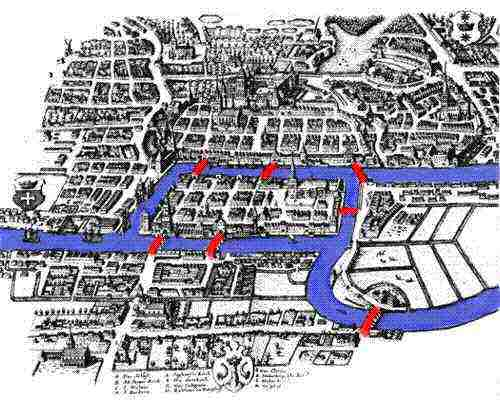
\includegraphics[scale=0.5]{Konigsberg.jpeg}
  \caption{A cidade de Königsberg e suas sete pontes}
\end{figure}

Segundo histórias, um passatempo de domingo dos cidadãos de Königsberg consistia em
passear por sua cidade, até que um dia surgiu um desafio: encontrar uma forma
de andar por todas as regiões passando por cada ponte apenas uma vez.

Nenhum habitante de Königsberg conseguiu encontrar a solução para este problema,
porém, o desafio chegou até um homem chamado Leonhard Euler, que apesar de julgar
o problema trivial, ficou intrigado, como citado em \citet{hopkins04:the}:

\begin{quotation}
  \emph{``This question is so banal, but seemed to me worthy of attention in that 
  [neither] geometry, nor algebra, nor even the art of counting was sufficient to
  solve it.''}
\end{quotation}

Euler provou que não era possível passar por toda a cidade de Königsberg sem passar
duas vezes pela mesma ponte, mas também resolveu o caso geral,
para qualquer número de regiões e qualquer número de pontes, dando assim origem
a um ramo da matemática que hoje chamamos de \textbf{Teoria dos Grafos}.

\section{Grafos}

Podemos definir um \textbf{Grafo} informalmente como um conjunto de entidades
conectadas entre si (ou não). Mais formalmente, podemos definir um grafo $G$ como um
par $(V, E)$ onde $V$ é um conjunto de \textbf{vértices} e $E$ um conjunto de
\textbf{arestas} entre os vértices tal que $E \subseteq \{ (u, v) \mid u, v \in V \}$.

As arestas de um grafo podem ter propriedades como direção e/ou algum valor
associado dependendo do contexto em que está sendo utilizado, frequentemente
possibilitando soluções elegantes e eficientes para os mais diversos problemas.

\begin{figure}
  \centering

  \begin{subfigure}{0.4\textwidth}
    \centering
    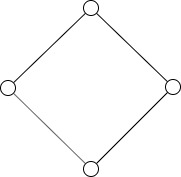
\includegraphics[width=.7\textwidth]{graph.jpg}
    \caption{Um grafo não dirigido.\label{fig:subfigures:a}}
  \end{subfigure}
  % ATENÇÃO: Se você deixar uma linha em branco entre as subfiguras,
  % LaTeX vai considerar que cada uma delas pertence a um "parágrafo"
  % diferente e, portanto, vai colocá-las em linhas separadas ao invés
  % de lado a lado.
  \begin{subfigure}{0.4\textwidth}
    \centering
    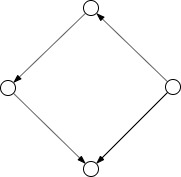
\includegraphics[width=.7\textwidth]{directed_graph.jpg}
    \caption{Um grafo dirigido.\label{fig:subfigures:b}}
  \end{subfigure}

  \begin{subfigure}{0.4\textwidth}
    \centering
    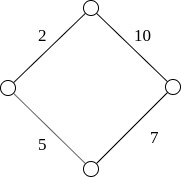
\includegraphics[width=.7\textwidth]{weighted_graph.jpg}
    \caption{Um grafo com valores nas arestas.\label{fig:subfigures:c}}
  \end{subfigure}
  \begin{subfigure}{0.4\textwidth}
    \centering
    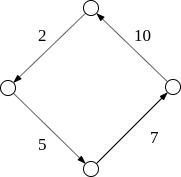
\includegraphics[width=.7\textwidth]{weighted_directed_graph.jpg}
    \caption{Um grafo dirigido com valores nas arestas.\label{fig:subfigures:d}}
  \end{subfigure}

  \caption{Exemplos de grafos.\label{fig:subfigures}}
\end{figure}

\section{Árvores}

\textbf{Árvores} são um subconjunto dos grafos de incrível importância para a
Ciência da Computação, sendo usadas nas mais diversas aplicações, desde a estrutura
de pastas de um sistema operacional até bancos de dados e processamento de
linguagem natural.

Diferente de outras estruturas como vetores, as árvores se organizam de forma
não linear, hierárquica. Os elementos de uma árvore são chamados de \textbf{nós} e
comumente um nó específico é elegido para ser a sua \textbf{raíz}. Cada nó pode
ter ligações com outros nós denominados \textbf{filhos}, que por sua vez podem
ter seus próprios filhos e assim sucessivamente até chegarmos em nós que não
possuem ligação com nenhum outro elemento; chamamos estes nós de \textbf{folhas}.

\begin{tikzpicture}[level/.style={sibling distance=60mm/#1}]
\node [circle,draw] (z){$n$}
  child {node [circle,draw] (a) {$\frac{n}{2}$}
    child {node [circle,draw] (b) {$\frac{n}{2^2}$}
      child {node {$\vdots$}
        child {node [circle,draw] (d) {$\frac{n}{2^k}$}}
        child {node [circle,draw] (e) {$\frac{n}{2^k}$}}
      } 
      child {node {$\vdots$}}
    }
    child {node [circle,draw] (g) {$\frac{n}{2^2}$}
      child {node {$\vdots$}}
      child {node {$\vdots$}}
    }
  }
  child {node [circle,draw] (j) {$\frac{n}{2}$}
    child {node [circle,draw] (k) {$\frac{n}{2^2}$}
      child {node {$\vdots$}}
      child {node {$\vdots$}}
    }
  child {node [circle,draw] (l) {$\frac{n}{2^2}$}
    child {node {$\vdots$}}
    child {node (c){$\vdots$}
      child {node [circle,draw] (o) {$\frac{n}{2^k}$}}
      child {node [circle,draw] (p) {$\frac{n}{2^k}$}
        child [grow=right] {node (q) {$=$} edge from parent[draw=none]
          child [grow=right] {node (q) {$O_{k = \lg n}(n)$} edge from parent[draw=none]
            child [grow=up] {node (r) {$\vdots$} edge from parent[draw=none]
              child [grow=up] {node (s) {$O_2(n)$} edge from parent[draw=none]
                child [grow=up] {node (t) {$O_1(n)$} edge from parent[draw=none]
                  child [grow=up] {node (u) {$O_0(n)$} edge from parent[draw=none]}
                }
              }
            }
            child [grow=down] {node (v) {$O(n \cdot \lg n)$}edge from parent[draw=none]}
          }
        }
      }
    }
  }
};
\path (a) -- (j) node [midway] {+};
\path (b) -- (g) node [midway] {+};
\path (k) -- (l) node [midway] {+};
\path (k) -- (g) node [midway] {+};
\path (d) -- (e) node [midway] {+};
\path (o) -- (p) node [midway] {+};
\path (o) -- (e) node (x) [midway] {$\cdots$}
  child [grow=down] {
    node (y) {$O\left(\displaystyle\sum_{i = 0}^k 2^i \cdot \frac{n}{2^i}\right)$}
    edge from parent[draw=none]
  };
\path (q) -- (r) node [midway] {+};
\path (s) -- (r) node [midway] {+};
\path (s) -- (t) node [midway] {+};
\path (s) -- (l) node [midway] {=};
\path (t) -- (u) node [midway] {+};
\path (z) -- (u) node [midway] {=};
\path (j) -- (t) node [midway] {=};
\path (y) -- (x) node [midway] {$\Downarrow$};
\path (v) -- (y)
  node (w) [midway] {$O\left(\displaystyle\sum_{i = 0}^k n\right) = O(k \cdot n)$};
\path (q) -- (v) node [midway] {=};
\path (e) -- (x) node [midway] {+};
\path (o) -- (x) node [midway] {+};
\path (y) -- (w) node [midway] {$=$};
\path (v) -- (w) node [midway] {$\Leftrightarrow$};
\path (r) -- (c) node [midway] {$\cdots$};
\end{tikzpicture}

Também definimos a \textbf{profundidade} de um nó como a quantidade
de arestas no caminho da raíz até ele. A raíz tem profundidade zero,
seus filhos profundidade um e assim sucessivamente.

\begin{figure}
  \centering
  \begin{tikzpicture}[
    level distance=1.5cm,
    level 1/.style={sibling distance=3cm},
    level 2/.style={sibling distance=1.5cm}]
    \node [circle, draw] {1}
      child {node [circle, draw] {2}
        child {node [circle, draw] {4}}
        child {node [circle, draw] {5}}
      }
      child {node [circle, draw] {3}
      child {node [circle, draw] {6}}
        child {node [circle, draw] {7}
        child [grow=right] {node (q) {$\qquad$} edge from parent[draw=none]
            child [grow=right] {node (q) {profundidade = 2} edge from parent[draw=none]
              child [grow=up] {node (r) {profundidade = 1} edge from parent[draw=none]
                child [grow=up] {node (s) {profundidade = 0} edge from parent[draw=none]
                }
              }
            }
          }
        }
      };
  \end{tikzpicture}
  \caption{O nó 1 é a raíz e tem como filhos os nós 2 e 3, cujos
  filhos são as folhas 4, 5 e 6, 7, respectivamente.}
  \end{figure}

\newpage

% Escrever bem é uma arte que exige muita técnica e dedicação e,
% consequentemente, há vários bons livros sobre como escrever uma boa
% dissertação ou tese. Um dos trabalhos pioneiros e mais conhecidos nesse
% sentido é o livro de
% %Umberto Eco~\cite{eco:09} % usando o estilo alpha
% Umberto~\citet{eco:09} % usando o estilo plainnat
% intitulado \emph{Como se faz uma tese}; é uma leitura bem interessante mas,
% como foi escrito em 1977 e é voltado para trabalhos de graduação na Itália,
% não se aplica tanto a nós.

% Sobre a escrita acadêmica em geral, John Carlis disponibilizou um texto curto
% e interessante~\citep{carlis:09} em que advoga a preparação de um único
% rascunho da tese antes da versão final. Mais importante que isso, no
% entanto, são os vários \textit{insights} dele sobre a escrita acadêmica.
% Dois outros bons livros sobre o tema são \emph{The Craft of Research}~\citep{craftresearch}
% e \emph{The Dissertation Journey}~\citep{dissertjourney}. Além disso, a USP
% tem uma compilação de normas relativas à produção de documentos
% acadêmicos~\citep{usp:guidelines} que pode ser utilizada como referência.

% Para a escrita de textos especificamente sobre Ciência da Computação, o
% livro de Justin Zobel, \emph{Writing for Computer Science}~\citep{zobel:04}
% é uma leitura obrigatória. O livro \emph{Metodologia de Pesquisa para
% Ciência da Computação} de
% %Raul Sidnei Wazlawick~\cite{waz:09} % usando o estilo alpha
% Raul Sidnei~\citet{waz:09} % usando o estilo plainnat
% também merece uma boa lida. Já para a área de Matemática, dois livros
% recomendados são o de Nicholas Higham, \emph{Handbook of Writing for
% Mathematical Sciences}~\citep{Higham:98} e o do criador do \TeX{}, Donald
% Knuth, juntamente com Tracy Larrabee e Paul Roberts, \emph{Mathematical
% Writing}~\citep{Knuth:96}.

% Apresentar os resultados de forma simples, clara e completa é uma tarefa que
% requer inspiração. Nesse sentido, o livro de
% %Edward Tufte~\cite{tufte01:visualDisplay}, % usando o estilo alpha
% Edward~\citet{tufte01:visualDisplay}, % usando o estilo plainnat
% \emph{The Visual Display of Quantitative Information}, serve de ajuda na
% criação de figuras que permitam entender e interpretar dados/resultados de forma
% eficiente.

% Além desse material, também vale muito a pena a leitura do trabalho de
% %Uri Alon \cite{alon09:how}, % usando o estilo alpha
% Uri \citet{alon09:how}, % usando o estilo plainnat
% no qual apresenta-se uma reflexão sobre a utilização da Lei de Pareto para
% tentar definir/escolher problemas para as diferentes fases da vida acadêmica.
% A direção dos novos passos para a continuidade da vida acadêmica deveria ser
% discutida com seu orientador.

% %% ------------------------------------------------------------------------- %%
% \section{Considerações de Estilo}
% \label{sec:consideracoes_preliminares}

% Normalmente, as citações não devem fazer parte da estrutura sintática da
% frase\footnote{E não se deve abusar das notas de rodapé.\index{Notas de rodapé}}.
% No entanto, usando referências em algum estilo autor-data (como o estilo
% plainnat do \LaTeX{}), é comum que o nome do autor faça parte da frase. Nesses
% casos, pode valer a pena mudar o formato da citação para não repetir o nome do
% autor; no \LaTeX{}, isso pode ser feito usando os comandos
% \textsf{\textbackslash{}citet}, \textsf{\textbackslash{}citep},
% \textsf{\textbackslash{}citeyear} etc. documentados no pacote
% natbib \citep{natbib}\index{natbib} (esses comandos são compatíveis com biblatex
% usando a opção \textsf{natbib=true}, ativada por padrão neste modelo). Em geral,
% portanto, as citações devem seguir estes exemplos:

% \small
% \begin{verbatim}
% Modos de citação:
% indesejável: [AF83] introduziu o algoritmo ótimo.
% indesejável: (Andrew e Foster, 1983) introduziram o algoritmo ótimo.
% certo: Andrew e Foster introduziram o algoritmo ótimo [AF83].
% certo: Andrew e Foster introduziram o algoritmo ótimo (Andrew e Foster, 1983).
% certo (\citet ou \citeyear): Andrew e Foster (1983) introduziram o algoritmo ótimo.
% \end{verbatim}
% \normalsize

% O uso desnecessário de termos em língua estrangeira deve ser evitado. No entanto,
% quando isso for necessário, os termos devem aparecer \textit{em itálico}.
% \index{Língua estrangeira}
% % index permite acrescentar um item no indice remissivo

% Uma prática recomendável na escrita de textos é descrever as
% legendas\index{Legendas} das figuras e tabelas em forma auto-contida: as
% legendas devem ser razoavelmente completas, de modo que o leitor possa entender
% a figura sem ler o texto onde a figura ou tabela é citada.\index{Floats}

% Sugerimos que você faça referências bibliográficas de forma similar aos
% estilos ``alpha'' (referências alfanuméricas) ou ``plainnat'' (referências
% por autor-data) de \LaTeX{}.  Se estiver usando natbib+bibtex\index{natbib}\index{bibtex},
% use os arquivos .bst ``alpha-ime.bst'' ou ``plainnat-ime.bst'', que são
% versões desses dois formatos traduzidas para o português. Se estiver usando
% biblatex\index{biblatex} (recomendado), escolha o estilo ``alphabetic''
% (que é um dos estilos padrão do biblatex) ou ``plainnat-ime''. O arquivo de
% exemplo inclui todas essas opções; basta des-comentar as linhas
% correspondentes e, se necessário, modificar o arquivo Makefile para chamar
% o bibtex\index{bibtex} ao invés do biber\index{biber} (este último é usado
% em conjunto com o biblatex).

% \section{Ferramentas Bibliográficas}

% Embora seja possível pesquisar por material acadêmico na Internet usando sistemas
% de busca ``comuns'', existem ferramentas dedicadas, como o \textsf{Google Scholar}\index{Google Scholar}
% (\url{scholar.google.com}). Você também pode querer usar o \textsf{Web of Science}\index{Web of Science}
% (\url{webofscience.com}) e o \textsf{Scopus}\index{Scopus} (\url{scopus.com}), que oferecem
% recursos sofisticados e limitam a busca a periódicos com boa reputação acadêmica.
% Essas duas plataformas não são gratuitas, mas os alunos da USP têm acesso a elas
% através da instituição. Ambas são capazes de exportar os dados para o formato .bib,
% usado pelo \LaTeX{}. Algumas editoras, como a ACM e a IEEE, também têm sistemas de
% busca bibliográfica.

% Apenas uma parte dos artigos acadêmicos de interesse está disponível livremente
% na Internet; os demais são restritos a assinantes. A CAPES assina um grande
% volume de publicações e disponibiliza o acesso a elas para diversas universidades
% brasileiras, entre elas a USP, através do seu portal de periódicos
% (\url{periodicos.capes.gov.br}). Existe uma extensão para os navegadores
% Chrome e Firefox (\url{www.infis.ufu.br/capes-periodicos}) que facilita o uso
% cotidiano do portal.

% Para manter um banco de dados organizado sobre artigos e outras fontes bibliográficas
% relevantes para sua pesquisa, é altamente recomendável que você use uma ferramenta
% como Zotero~(\url{zotero.org})\index{Zotero} ou
% Mendeley~(\url{mendeley.com})\index{Mendeley}. Ambas podem exportar seus dados no
% formato .bib, compatível com \LaTeX{}. Também existem três plataformas
% gratuitas que permitem a busca de referências acadêmicas já no formato .bib:

% \begin{itemize}
%   \item \emph{CiteULike}\index{CiteULike} (patrocinados por Springer): \url{www.citeulike.org}
%   \item Coleção de bibliografia em Ciência da Computação: \url{liinwww.ira.uka.de/bibliography}
%   \item Google acadêmico\index{Google Scholar} (habilitar bibtex nas preferências): \url{scholar.google.com}
% \end{itemize}

% Lamentavelmente, ainda não existe um mecanismo de verificação ou validação das
% informações nessas plataformas. Portanto, é fortemente sugerido validar todas
% as informações de tal forma que as entradas bib estejam corretas.

% De qualquer modo, tome muito cuidado na padronização das referências
% bibliográficas: ou considere TODOS os nomes dos autores por extenso, ou TODOS
% os nomes dos autores abreviados.  Evite misturas inapropriadas.

% \section{O Que o IME Espera}

% Ao terminar sua tese/dissertação, você deve entregar uma cópia dela para a
% CPG. Após a defesa, você tem 30 dias para revisar o texto e incorporar as
% sugestões da banca. Assim, há duas versões oficiais do documento: a versão
% original e a versão corrigida, o que deve ser indicado na folha de rosto.
% \index{Tese/Dissertação!versões}

% Fica a critério do aluno definir aspectos como o tamanho de fonte, margens,
% espaçamento, estilo de referências, cabeçalho, etc. considerando sempre o
% bom senso. A CPG, em reunião realizada em junho de 2007, aprovou que as
% teses/dissertações deverão seguir o formato padrão por ela
% definido\footnote{\url{www.ime.usp.br/dcc/pos/normas/tesesedissertacoes}}.
% Esse padrão refere-se aos itens que devem estar presentes nas teses/dissertações
% (e.g. capa, formato de rosto, sumário, etc.), e não à formatação do documento.
% Ele define itens obrigatórios e opcionais, conforme segue:\index{Formatação}
% \index{Tese/Dissertação!itens obrigatórios}
% \index{Tese/Dissertação!itens opcionais}

% \begin{itemize}
%   \item \textsc{Capa} (obrigatória)
%   \begin{itemize}
%     \item O IME usa uma capa padrão de cartolina para todas as
%     teses/dissertações.  Essa capa tem uma janela recortada por onde se
%     vê o título e o autor do trabalho e, portanto, a capa impressa do
%     trabalho deve incluir o título e o autor na posição correspondente da
%     página. Ela fica centralizada na página, tem 100mm de largura, 60mm de
%     altura e começa 47mm abaixo do topo da página.

%     \item O título da tese/dissertação deverá começar com letra maiúscula
%     e o resto deverá ser em minúsculas, salvo nomes próprios.

%     \item O nome do aluno(a) deverá ser completo e sem abreviaturas.

%     \item É preciso explicitar se é uma tese ou dissertação (para
%     obtenção do título de doutor, tese; para obtenção do título de
%     mestre, dissertação).

%     \item O nome do programa deve constar da capa (Matemática,
%     Matemática Aplicada, Estatística ou Ciência da Computação).

%     \item Também devem constar o nome completo do orientador e do
%     co-orientador, se houver.

%     \item Se o aluno recebeu bolsa, deve-se indicar a(s) agência(s).

%     \item É preciso informar o mês e ano do depósito ou da entrega da
%     versão corrigida.
%   \end{itemize}

%   \item \textsc{Folha de Rosto} (obrigatória, tanto para a versão
%   depositada quanto para a versão corrigida)
%   \begin{itemize}
%     \item o título da tese/dissertação deverá seguir o padrão da capa

%     \item deve informar se se trata da versão original ou da versão
%     corrigida; no segundo caso, deve também incluir os nomes
%     dos membros da banca.
%   \end{itemize}

%   \item \textsc{Agradecimentos} (opcional)

%   \item \textsc{Resumo}, em português (obrigatório)

%   \item \textsc{Abstract}, em inglês (obrigatório)

%   \item \textsc{Sumário} (obrigatório)

%   \item \textsc{Listas} (opcionais)
%   \begin{itemize}
%     \item Lista de Abreviaturas
%     \item Lista de Símbolos
%     \item Lista de Figuras
%     \item Lista de Tabelas
%   \end{itemize}

%   \item \textsc{Referências Bibliográficas} (obrigatório)

%   \item \textsc{Índice Remissivo} (opcional\footnote{O índice remissivo
%    pode ser muito útil para a banca; assim, embora seja um item opcional,
%    recomendamos que você o crie.})
% \end{itemize}

\par

%!TeX root=../tese.tex
%("dica" para o editor de texto: este arquivo é parte de um documento maior)
% para saber mais: https://tex.stackexchange.com/q/78101/183146

\chapter{O problema do Ancestral de Nível}
Uma consulta Ancestral de Nível $\mathrm{AN}(u, d)$ 

\newpage

\begin{program}   
      \lstinputlisting[
        language=pseudocode,
        style=pseudocode,
        style=wider,
        functions={},
        specialidentifiers={},
      ]
      {conteudo-exemplo/euclid.psc}
    
      \caption{Máximo divisor comum (arquivo importado).\label{prog:mdcinput}}
    \end{program}

\begin{program}
      \lstinputlisting[
        language=pseudocode,
        style=pseudocode,
        style=wider,
        functions={parent, depth},
        specialidentifiers={},
      ]
      {conteudo-exemplo/naive_query.psc}
    
      \caption{Naïve Algorithm query.\label{prog:mdcinput}}
    \end{program}

\newpage
%\chapter{Usando o \LaTeX{} e este modelo}

Não é necessário que o texto seja redigido usando \LaTeX{}, mas é fortemente
recomendado o uso dessa ferramenta, pois ela facilita diversas etapas do
trabalho e o resultado final é muito bom\footnote{O uso de um sistema de
controle de versões, como mercurial (\url{mercurial-scm.org}) ou git
(\url{git-scm.com}), também é altamente recomendado.}. Este modelo inclui
vários comentários explicativos e pacotes interessantes para auxiliá-lo com
ele, sendo composto dos arquivos principais de cada exemplo
(\texttt{tese.tex}, \texttt{artigo.tex},
\texttt{apresentacao.tex} e \texttt{poster.tex}) e de
vários arquivos auxiliares:

\begin{itemize}
  \item Arquivos com o conteúdo do trabalho:
  \begin{itemize}
    \item \texttt{conteudo/folhas-de-rosto.tex} (capa, dedicatória etc.)
    \item \texttt{conteudo/resumo-abstract.tex}
    \item \texttt{conteudo/capitulos.tex}, \texttt{conteudo/apendices.tex},
          \texttt{conteudo/anexos.tex} e demais arquivos carregados por eles
          (\texttt{XX-*.tex}, \texttt{apendice-pseudocodigo.tex}, \texttt{anexo-soft-livre.tex})
    \item \texttt{bibliografia.bib} (dados bibliográficos)
  \end{itemize}

  \item Arquivos com as \textit{packages} usadas e suas configurações (leia
        os comentários neles se quiser modificar algum aspecto do
        documento ou acrescentar alguma \textit{package}):
  \begin{itemize}
    \item \texttt{extras/basics.tex} (\textit{packages} e configurações essenciais),
          \texttt{extras/fonts.tex} (definição das fontes do documento) e
          \texttt{extras/floats.tex} (configurações e melhorias para \textit{floats})
    \item \texttt{extras/thesis-formatting.tex} (aparência: espaçamento, sumário etc.)
    \item \texttt{extras/index.tex} (configuração do índice remissivo)
    \item \texttt{extras/hyperlinks.tex} (configuração das referências cruzadas)
    \item \texttt{extras/source-code.tex} (exibição de código-fonte e pseudocódigo)
    \item \texttt{extras/utils.tex} (\textit{packages} adicionais diversas)
    \item \texttt{extras/bibconfig.tex} (configuração da bibliografia)
  \end{itemize}

  \item Outros arquivos auxiliares (geralmente não precisam ser editados):
  \begin{itemize}
    \item \texttt{extras/imeusp-capa.sty} (formatação da capa e demais páginas iniciais)
    \item \texttt{extras/imeusp-headers.sty} (formatação dos cabeçalhos)
    \item \texttt{extras/lstpseudocode.sty} (suporte a pseudocódigo com \textsf{listings})
    \item \texttt{extras/annex.sty} (permite adicionar anexos) e
          \texttt{extras/appendixlabel.sty} (melhora a lista de
          apêndices/anexos no sumário)
    \item \texttt{extras/beamer*.sty} (\textit{layouts} e cores para
          apresentações e \textit{posters})
    \item \texttt{extras/plainnat-ime.*} (estilo plainnat para bibliografias)\index{biblatex}
    \item \texttt{extras/alpha-ime.bst} (estilo alpha para bibliografias com
          bibtex)\index{bibtex}
    \item \texttt{extras/natbib-ime.sty} (tradução da \textit{package}
          padrão natbib)\index{natbib}
    \item \texttt{hyperxindy.xdy} (configuração para xindy) e
          \texttt{mkidxhead.ist} (configuração para makeindex)
    \item \texttt{latexmkrc} e \texttt{Makefile} (automatizam a geração do
          documento com os comandos \textsf{latexmk} e \textsf{make} respectivamente)
  \end{itemize}
\end{itemize}

Para compilar o documento, basta executar o comando \textsf{latexmk} (ou
\textsf{make})\footnote{Você também pode usar \textsf{latexmk poster},
\textsf{make apresentacao} etc.}. Talvez seu editor ofereça uma
opção de menu para compilar o documento, mas ele provavelmente depende do
\textsf{latexmk} para isso. \LaTeX{} gera diversos arquivos auxiliares
durante a compilação que, em algumas raras situações, podem ficar
inconsistentes (causando erros de compilação ou erros no PDF gerado, como
referências faltando ou numeração de páginas incorreta no sumário). Nesse
caso, é só usar o comando \textsf{latexmk -C} (ou \textsf{make clean}),
que apaga todos os arquivos auxiliares gerados, e em seguida rodar
\textsf{latexmk} (ou \textsf{make}) novamente.

\section{Instalação do \LaTeX{}}
\label{sec:install}

\enlargethispage{-.5\baselineskip}

\LaTeX{} é, na verdade, um conjunto de programas. Ao invés de procurar e
baixar cada um deles, o mais comum é baixar um pacote com todos eles juntos.
Há dois pacotes desse tipo disponíveis: MiK\TeX{} (\url{miktex.org}) e
\TeX{}Live (\url{www.tug.org/texlive}). Ambos funcionam em Linux, Windows e
MacOS X. Em Linux, \TeX{}Live costuma estar disponível para instalação junto
com os demais opcionais do sistema. Em MacOS X, o mais popular é o Mac\TeX{}
(\url{www.tug.org/mactex/}), a versão do \TeX{}Live para MacOS X.  Em Windows,
o mais comumente usado é o MiK\TeX{}.

Por padrão, eles não instalam tudo que está disponível, mas sim apenas os
componentes mais usados, e oferecem um gestor de pacotes que permite adicionar
outros. Embora uma instalação completa do \LaTeX{} seja relativamente grande
(perto de 5GB), em geral vale a pena instalar a maior parte dos pacotes. Se
você preferir uma instalação mais ``enxuta'', não deixe de incluir todos os
pacotes necessários para este modelo, como indicado no arquivo README.md.

Também é muito importante ter o \textsf{latexmk} (ou o \textsf{make}). No Linux,
a instalação é similar à de outros programas. No MacOS X e no Windows,
\textsf{latexmk} pode ser instalado pelo gestor de pacotes do MiK\TeX{} ou
\TeX{}Live. Observe que ele depende da linguagem \textsf{perl}, que precisa ser
instalada à parte no Windows (\url{www.perl.org/get.html}).

\section{Documentação sobre \LaTeX}
\label{sec:docs}

Existem diversos bons livros sobre \LaTeX{} (embora em geral um tanto
antigos), dos quais destacamos dois:

\begin{enumerate}

  \item A quarta edição de ``A Guide to \LaTeX'', de Helmut Kopka e
        Patrick W. Daly (publicada em 2003), além de uma ótima
        introdução, aborda vários tópicos relativamente avançados e
        úteis\footnote{Um dos autores disponibiliza uma versão não-final
        em \url{www2.mps.mpg.de/homes/daly/GTL/gtl_20030512.pdf}.}.
  \item A segunda edição de ``The \LaTeX{} Companion'' (publicada em
        2004) é um livro quase obrigatório, pois discute em detalhes
        praticamente todos os recursos e \textit{packages} importantes
        de \LaTeX{}, servindo tanto para o aprendizado quanto como
        material de referência.

\end{enumerate}

\enlargethispage{-.5\baselineskip}

Além de livros, há muito material sobre \LaTeX{} na Internet, mas também há
muita informação obsoleta. Em particular, você pode ignorar explicações sobre
como converter arquivos no formato DVI gerados por \LaTeX{} em PDF: versões
modernas de \LaTeX{} geram arquivos PDF diretamente. Quanto a imagens, os
formatos de arquivo PS/EPS (PostScript e Encapsulated PostScript) não são mais
aceitos; hoje em dia \LaTeX{} trabalha com arquivos de imagem nos formatos PDF,
PNG e JPEG. Finalmente, recursos gráficos não usam mais \textit{packages} como
\textsf{pstricks}, \textsf{eepic} ou outras tradicionalmente citadas; ao invés
disso, \textsf{PGF/TikZ} é a ferramenta mais comum.

Dentre o material online, o conteúdo em \url{overleaf.com/learn} é excelente,
incluindo um rápido tutorial (de escopo similar ao Capítulo~\ref{chap:tutorial}
deste modelo) e várias páginas sobre como utilizar recursos específicos. Um
tutorial bastante abrangente e detalhado está disponível em
\url{tug.org/twg/mactex/tutorials/ltxprimer-1.0.pdf} (há outros, como
\url{tug.org/tutorials/tugindia},
\url{www.maths.tcd.ie/~dwilkins/LaTeXPrimer/GSWLaTeX.pdf} e
\url{www.andy-roberts.net/writing/latex}). Em português, você pode consultar
\url{polignu.org/sites/polignu.org/files/latex/latex-fflch.pdf} e
\url{git.febrace.org.br/material-latex/material-latex} (este precisa ser
baixado e compilado). O sítio \url{tex.stackexchange.com} é
um fórum de perguntas e respostas sobre \LaTeX{} muito útil, pois os
principais desenvolvedores do sistema participam das discussões, e o sítio
\url{texfaq.org} é bastante abrangente e atualizado. O canal
\url{youtube.com/c/anteroneves} tem vários vídeos instrutivos em português.

Como dito anteriormente, \LaTeX{} é, na verdade, um conjunto de programas e,
normalmente, instalamos pacotes pré-prontos com todos eles. Esses pacotes (em
geral, \TeX{}Live e MiK\TeX{}) contém também a documentação das
\textit{packages} incluídas: Basta digitar \textsf{texdoc nome-da-package}
(\TeX{}Live) ou \textsf{mthelp nome-da-package} (MiK\TeX{}) para ter acesso à
documentação correspondente. \textsf{texdoc/mthelp} incluem também alguns
tutoriais e textos introdutórios, como ``The Not So Short Introduction to
\LaTeXe{}'' (\textsf{texdoc lshort-eng}; há uma versão em português, mas não
está em dia com o original), ``Getting up and running with \AmS-\LaTeX{}''
(\textsf{texdoc amshelp}) e ``A Simplified Introduction to \LaTeX{}''
(\textsf{texdoc simplified-intro}). Versões recentes do \LaTeX{} incluem
também o ``\LaTeXe{} via exemplos'' (\textsf{texdoc latex-via-exemplos}),
em português. O sítio \url{texdoc.net} oferece acesso online a essa mesma
documentação de maneira organizada e o sítio \url{ctan.org} é o
repositório semi-oficial das \textit{packages} \LaTeX{} e sua documentação.

A documentação de referência de \LaTeX{} pode ser acessada com \textsf{texdoc
latex2e} e \textsf{texdoc source2e}; a documentação de referência das classes
padrão (\textsf{article, book etc}), por sua vez, com \textsf{texdoc classes}.
Você normalmente não vai usá-las, mas elas podem servir para esclarecer algum
detalhe. \textsf{texdoc clsguide} é um guia para a criação de novas classes e
\textit{packages}, e \textsf{texdoc fntguide} explica como funciona a gestão
de fontes de \LaTeX{} (mas note que \LuaLaTeX{} e \XeLaTeX{} usam outro
mecanismo). Você pode ver exemplos de fontes disponíveis para \LaTeX{} em
\url{tug.org/FontCatalogue}.

Quando você se tornar um usuário avançado, pode se interessar em conhecer
melhor a linguagem \TeX{}, que está na base do \LaTeX{}. ``The \TeX{} book'',
de Donald Knuth, é amplamente recomendado, mas há três livros completos a
respeito que são instalados com \LaTeX{}: ``A gentle introduction to \TeX{}''
(\textsf{texdoc gentle}), ``\TeX{} for the impatient'' (\textsf{texdoc
impatient}) e ``\TeX{} by topic'' (\textsf{texdoc texbytopic}).

\par

%!TeX root=../tese.tex
%("dica" para o editor de texto: este arquivo é parte de um documento maior)
% para saber mais: https://tex.stackexchange.com/q/78101/183146

% Vamos definir alguns comandos auxiliares para facilitar.

% "textbackslash" é muito comprido.
\newcommand{\sla}{\textbackslash}

% Vamos escrever comandos (como "make" ou "itemize") com formatação especial.
\newcommand{\cmd}[1]{\textsf{#1}}

% Idem para packages; aqui estamos usando a mesma formatação de \cmd,
% mas poderíamos escolher outra.
\newcommand{\pkg}[1]{\textsf{#1}}

% A maioria dos comandos LaTeX começa com "\"; vamos criar um
% comando que já coloca essa barra e formata com "\cmd".
\newcommand{\ltxcmd}[1]{\cmd{\sla{}#1}}

\chapter{O Problema do Ancestral de Nível e Implementações}
\label{chap:implementacoes}

\section{Definição do problema}
O problema do \textbf{Ancestral de Nível} é um problema fundamental de árvores que pode
ser definido da seguinte forma: Dada uma árvore enraizada $T$ com $n$ nós, para
consultas $\mathrm{AN}(u, d)$ onde $u$ é um nó de $T$ e $d$ um número inteiro,
encontre o ancestral de profundidade $d$ de $u$ otimizando tanto o tempo de
preprocessamento quanto o de resposta às consultas.

\tikzset{
  treenode/.style = {align=center, minimum size=7mm, inner sep=0pt, text centered},
  arn_n/.style = {treenode, circle, white, font=\bfseries, draw=black,
    fill=black, text width=1.5em},% arbre rouge noir, noeud noir
  arn_r/.style = {treenode, circle, red, draw=red, 
    text width=1.5em, very thick},% arbre rouge noir, noeud rouge
  arn_x/.style = {treenode, circle, draw=black, minimum size=7mm}% arbre rouge noir, nil
}

\begin{figure}[H]
    \begin{tikzpicture}[scale=0.7,
      level distance=1.5cm,
      level 1/.style={sibling distance=6cm},
      level 2/.style={sibling distance=3cm},
      level 3/.style={sibling distance=1.5cm}]
      \node [arn_x] {0}
        child {node [arn_x] {1}
          child {node [arn_x] {3}
            child {node [arn_x] {7}}
            child {node [arn_x] {8}}
          }
          child {node [arn_x] {4}
            child {node [arn_x] {9}}
            child {node [arn_x] {10}}
          }
        }
        child {node [arn_r] {2}
          child {node [arn_x] {5}
            child {node [arn_x] {11}}
            child {node [arn_x] {12}}
          }
          child {node [arn_x] {6}
              child {node [arn_n] {13}}
              child {node [arn_x] {14}}
          }
        };
    \end{tikzpicture}
    \caption[Exemplo de consulta de Ancestral de Nível]
    {Exemplo de consulta AN(13, 1) = 2.}
  \end{figure}

  \begin{figure}[H]
    \begin{tikzpicture}[scale=0.7,
        level distance=1.5cm,
        level 1/.style={sibling distance=6cm},
        level 2/.style={sibling distance=3cm},
        level 3/.style={sibling distance=1.5cm}]
        \node [arn_x] {0}
          child {node [arn_x] {1}
            child {node [arn_x] {3}
              child {node [arn_x] {7}}
              child {node [arn_x] {8}}
            }
            child {node [arn_r] {4}
              child {node [arn_n] {9}}
              child {node [arn_x] {10}}
            }
          }
          child {node [arn_x] {2}
            child {node [arn_x] {5}
              child {node [arn_x] {11}}
              child {node [arn_x] {12}}
            }
            child {node [arn_x] {6}
                child {node [arn_x] {13}}
                child {node [arn_x] {14}}
            }
          };
      \end{tikzpicture}
      \caption[Exemplo de consulta de Ancestral de Nível]
      {Exemplo de consulta AN(9, 2) = 4.}
    \end{figure}

Existem diversas soluções para tal problema, de diferentes níveis de complexidade e
com performances teoricamente diferentes. Em particular, por exemplo, é possível
realizar as consultas de forma trivial sem qualquer tipo de preprocessamento ou também
preprocessar todas as possíveis consultas para que possam então ser respondidas
rapidamente.

Em \citet{Bender2002TheLA}, \citet{LAInPractice} e \citet{menghani2019simple} são
discutidas algumas soluções, incluindo as que serão implementadas e testadas neste
trabalho. Em particular, preferi testar soluções que fossem razoavelmente simples
de serem implementadas, até mesmo para mostrar que estas são muitas vezes bastante
suficientes.

Como motivação para o estudo deste problema, vale lembrar que o Ancestral de Nível
aparece como parte de problemas mais complexos como árvores ordinais espaço-eficientes
como descrito em \citet{Geary:2006:SOT:1198513.1198516} que podem ser usadas na
representação de documentos XML que suportam consultas XPath. Além disso, são usadas
em \citet{Sadakane:2006:SSD:1109557.1109693} para implementar estruturas de dados
comprimidas e também em \citet{Yuan:2009:EDS:1514894.1514908} para consultas agregadas
em árvores. Por último, vemos aplicações até mesmo no campo de \textit{hashing} em
strings, como dito em \citet{10.1007/3-540-61258-0_11}.

\section{Implementações}

Todas as implementações assumem a mesma implementação de árvore onde é
guardada apenas sua raíz e cada nó contém um vetor de ponteiros para seus
filhos. Para facilitar as implementações, ao construir a árvore é feita uma
busca em profundidade para preencher vetores que servirão como funções globais
\texttt{pai()} e \texttt{profundidade()}.

\begin{program}[H]
  \lstinputlisting[
    language=pseudocode,
    style=pseudocode,
    style=wider,
    functions={travessia},
    specialidentifiers={global},
  ]
  {conteudo-exemplo/tree.psc}

  \caption{Criação da árvore.\label{prog:tree}}
\end{program}

Estamos interessados em analisar, para cada algoritmo, tanto sua complexidade de
tempo de execução quanto a de espaço adicional, também levando em consideração quão
simples é sua implementação.

Para tornar a discussão da complexidade de tempo mais clara, vamos dizer que se um
algoritmo tem complexidade de tempo $\langle f(x), g(x) \rangle$, a complexidade de
seu preprocessamento é $f(x)$ e de suas consultas é $g(x)$.

\subsection{Algoritmo Trivial}

O primeiro algoritmo a ser estudado é um em que simplesmente não há
nenhum preprocessamento e, para cada consulta, apenas subimos pelos pais a
partir do nó em questão até encontrarmos seu ancestral com profundidade igual
à profundidade requisitada.

%\subsection*{Preprocessamento}
Para esta implementação, o tempo de execução de seu preprocessamento não depende do
tamanho da árvore e também não utiliza nenhuma memória adicional, portanto o
preprocessamento do Algoritmo Trivial tem complexidade $\bigO(1)$ tanto para tempo
quanto espaço.

%\subsection*{Consultas}

No que diz respeito a cada consulta, precisamos chamar a função $pai()$
partindo do nó inicial até chegar no nó com a profundidade desejada.
Essa quantidade é exatamente a diferença entre esta profundidade e a
profundidade do nó inicial.

\begin{program}[]
  \lstinputlisting[
    language=pseudocode,
    style=pseudocode,
    style=wider,
    functions={pai, profundidade},
    specialidentifiers={},
  ]
  {conteudo-exemplo/naive_query.psc}

  \caption{Consulta do Algoritmo Trivial.\label{prog:naivequery}}
\end{program}

A consulta mais lenta para uma árvore qualquer é uma que parte do nó mais profundo
e precisa subir até a raíz, levando tempo $\bigO(d)$, onde $d$ é a profundidade
da árvore. No pior caso isso é equivalente a $\bigO(n)$ onde $n$ é a quantidade
de nós e para uma árvore balanceada cujos nós tem $k$ filhos, é equivalente a
$\bigO(\log_k n)$, fazendo com que a performance da consulta seja muito dependente da
forma da árvore.

Após essa análise, podemos concluir que o Algoritmo Trivial tem complexidade de tempo
$\langle \bigO(1), \bigO(d) \rangle$ e $\bigO(1)$ de espaço adicional, sendo
particularmente eficiente para árvores balanceadas e com fator de ramificação maior.


\subsection{Algoritmo da Tabela}
Ao contrário do algoritmo trivial, a ideia é precalcular o resultado de todas
as consultas possíveis durante a fase de preprocessamento para otimizar o
desempenho da fase de consultas.

Cada nó $u$ tem associado a si $profundidade(u) + 1$ possíveis consultas. Assim, para uma
árvore com $n$ nós, existem $n + \sum_{i=0}^{n-1} profundidade(i) = \bigO(nd)$ consultas, onde $d$ é a profundidade da árvore.
O preprocessamento se dá de maneira simples, preenchendo uma tabela de tamanho
$\bigO(nd)$ com dois laços encadeados, utilizando a função $pai()$ para subir a partir
de cada nó até a raíz e salvar a resposta para cada profundidade.

\begin{program}[]
  \lstinputlisting[
    language=pseudocode,
    style=pseudocode,
    style=wider,
    functions={pai, profundidade},
    specialidentifiers={},
  ]
  {conteudo-exemplo/table_preprocessing.psc}

  \caption{Preprocessamento do Algoritmo da Tabela.\label{prog:tableproc}}
\end{program}

Com a tabela devidamente preenchida, as consultas se tornam tão simples quanto acessar
a sua entrada correspondente, ou seja, a resposta da consulta que pede pelo ancestral
do nó $u$ com profundidade $p$ é dada por $tabela[u][p]$. 

\begin{program}[h!]
  \lstinputlisting[
    language=pseudocode,
    style=pseudocode,
    style=wider,
    functions={pai, profundidade},
    specialidentifiers={},
  ]
  {conteudo-exemplo/table_query.psc}

  \caption{Consulta do Algoritmo da Tabela.\label{prog:tablequery}}
\end{program}

A complexidade de espaço e de tempo do preprocessamento dependem fortemente da forma da
árvore, podendo ser $\bigO(n^2)$ no caso de uma árvore linear e para o caso de uma
árvore $k$-ária balanceada é $\bigO(n \log_k n)$, muito mais eficiente. Já a consulta
é feita em tempo $\bigO(1)$, sem uso de espaço adicional. Assim, o Algoritmo da Tabela
tem complexidade de tempo $\langle \bigO(nd), \bigO(1) \rangle$ e $\bigO(nd)$ de espaço,
sendo uma boa opção para casos de árvores balanceadas em que o preprocessamento se torna
barato frente à quantidade de consultas que serão feitas e o espaço utilizado não é
uma restrição.


\subsection{Algoritmo dos Ponteiros}
Essa é possivelmente a solução mais complexa que vamos analisar

\begin{program}[h!]
  \lstinputlisting[
    language=pseudocode,
    style=pseudocode,
    style=wider,
    functions={dfs, filhos, insere},
    specialidentifiers={global},
  ]
  {conteudo-exemplo/jump_preprocess.psc}

  \caption{Preprocessamento do Algoritmo da Preordem.\label{prog:preorderproc}}
\end{program}

\subsection{Algoritmo da Preordem}
O último algoritmo faz uso das propriedades da preordem de uma árvore para trazer uma
solução mais eficiente. Enquanto é feita a travessia da árvore cada nó é associado à
seu índice na preordem, que é inserido numa lista de nós de sua respectiva profundidade.

\begin{figure}
  \centering
  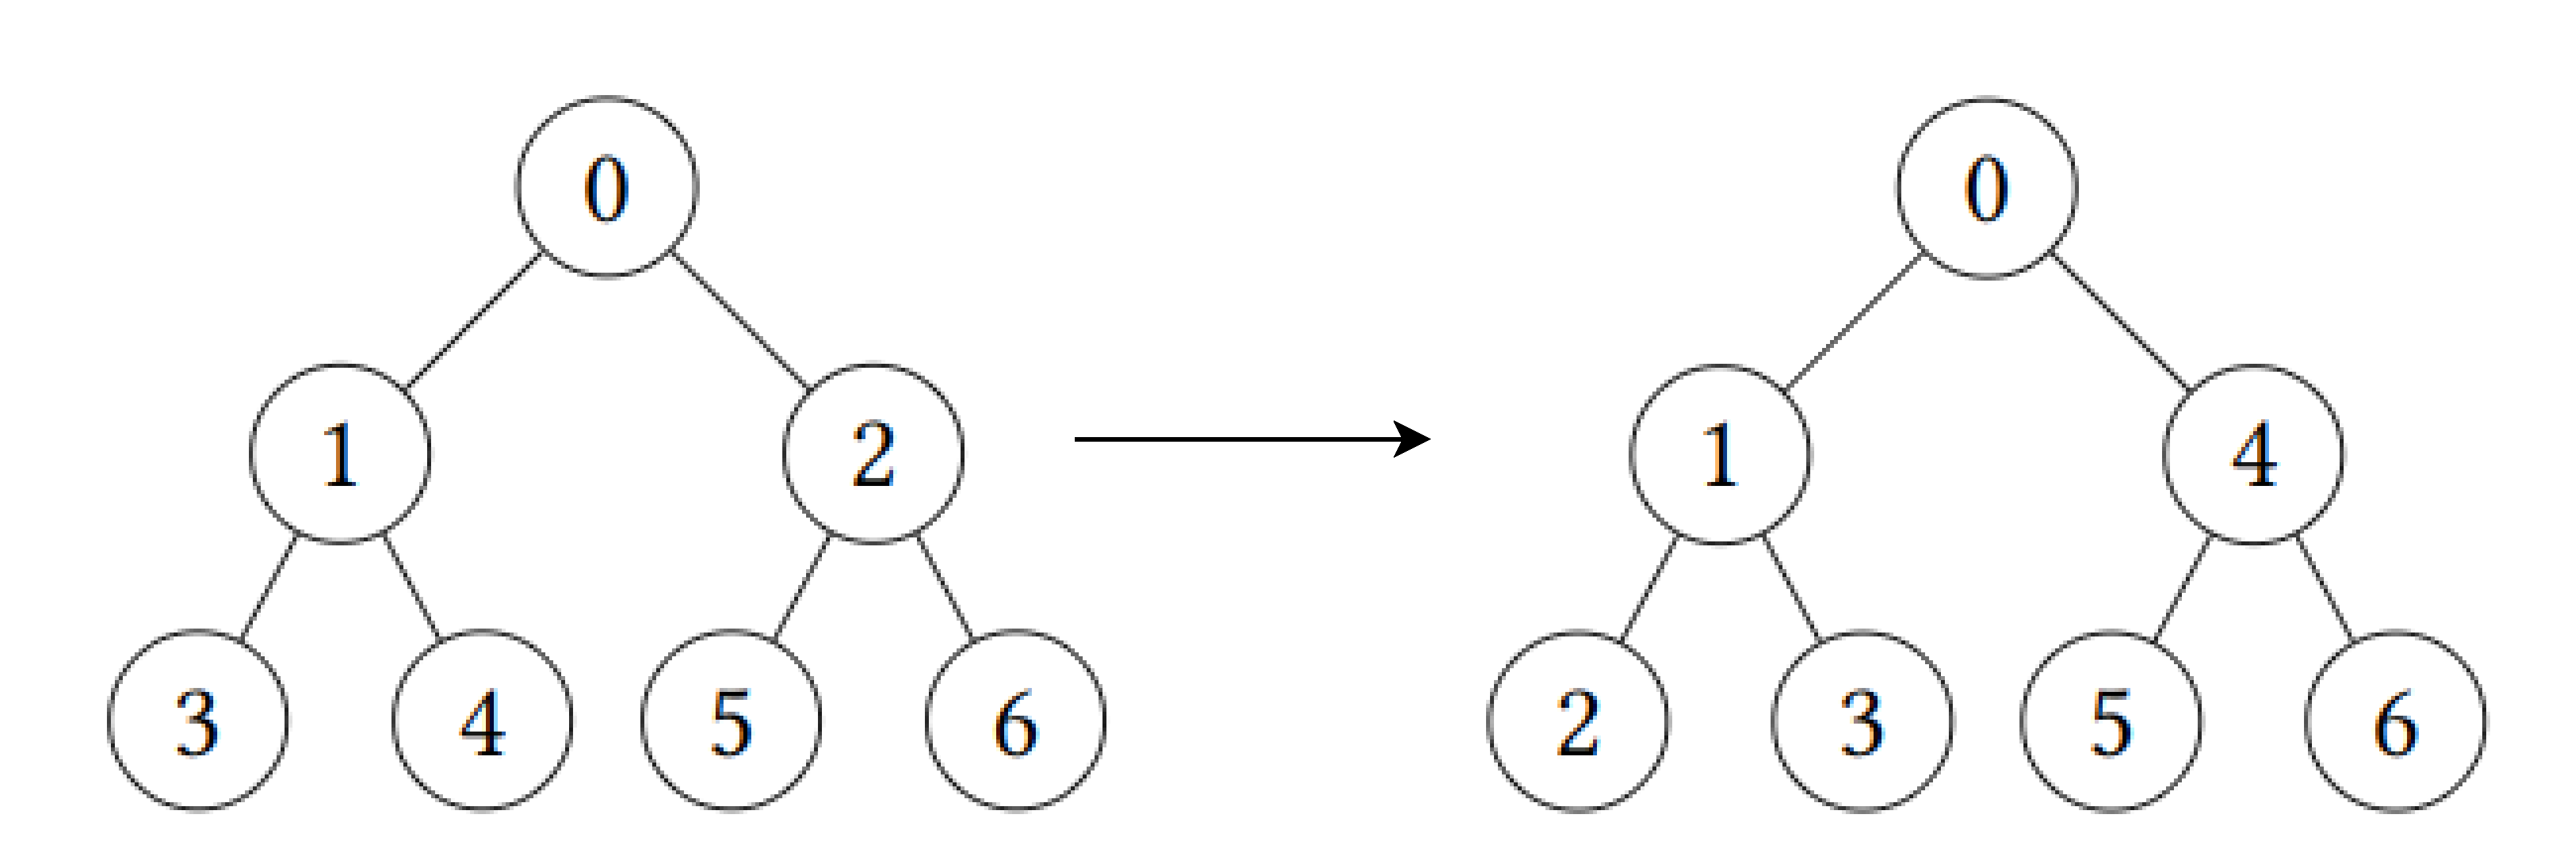
\includegraphics[scale=0.18]{preordertransformation.pdf}
  \caption{Associação entre os índices originais e os índices da preordem.}
\end{figure}

\begin{table}[]
  \begin{tabular}{llllll}
  \cline{3-3}
  profundidade 0: & \multicolumn{1}{l|}{} & \multicolumn{1}{l|}{0} &                        &                        &                        \\ \cline{3-3}
                  &                       &                        &                        &                        &                        \\ \cline{3-4}
  profundidade 1: & \multicolumn{1}{l|}{} & \multicolumn{1}{l|}{1} & \multicolumn{1}{l|}{4} &                        &                        \\ \cline{3-4}
                  &                       &                        &                        &                        &                        \\ \cline{3-6} 
  profundidade 2: & \multicolumn{1}{l|}{} & \multicolumn{1}{l|}{2} & \multicolumn{1}{l|}{3} & \multicolumn{1}{l|}{5} & \multicolumn{1}{l|}{6} \\ \cline{3-6} 
  \end{tabular}
  \caption[Vetores contendo os nós processados em cada nível.]
  {Vetores contendo os nós processados em cada nível. Os índices são referentes à preordem.}
\end{table}

Para tal, a ideia é guardar a ordem em que os nós de cada nível
foram visitados durante a travessia em preordem em vetores e então uma consulta se
resume a procurar o ancestral do nó inicial que está no vetor correspondente à
profundidade buscada.

\begin{program}[h!]
  \lstinputlisting[
    language=pseudocode,
    style=pseudocode,
    style=wider,
    functions={dfs, filhos, insere},
    specialidentifiers={global},
  ]
  {conteudo-exemplo/preorder_preprocess.psc}

  \caption{Preprocessamento do Algoritmo da Preordem.\label{prog:preorderproc}}
\end{program}

Para entendermos o funcionamento do algoritmo para as consultas, primeiro precisamos
nos convencer de que, se um nó $v$ é ancestral de $u$, então $preordem(v) < preordem(u)$,
onde $preordem(x)$ é o índice associado à posição de $x$ na travessia em preordem, já
que sempre descobrimos os filhos de um nó depois dele próprio. Além disso, no caso em
que existam vários nós em determinada profundidade, o ancestral que buscamos é aquele
cujo índice na preordem é o mais próximo do índice do nó inicial, porém ainda menor
que tal.

\begin{program}[]
  \lstinputlisting[
    language=pseudocode,
    style=pseudocode,
    style=wider,
    functions={upper_bound},
    specialidentifiers={},
  ]
  {conteudo-exemplo/preorder_query.psc}

  \caption{Consulta do Algoritmo da Preordem.\label{prog:preorderquery}}
\end{program}

\section{Considerações gerais}
No próximo capítulo estaremos interessados em avaliar a performance de cada algoritmo
para alguns casos de teste, levando em consideração o preprocessamento necessário,
a realização de consultas e a quantidade de memória utilizada.

Entretanto, analisando as tabelas ~\ref{tab:complexidadetempo},
~\ref{tab:complexidadeespaco} podemos perceber de imediato que restringir a entrada
para árvores balanceadas permite até mesmo que os algoritmos mais simples apresentem
complexidades boas, sendo ótimas opções levando em consideração também a dificuldade
de implementação de cada algoritmo.

\begin{table}[]
  \begin{tabular}{|c|l|l|l|}
  \hline
            & Linear                                       & Binária                                      & k-ária                                       \\ \hline
  Trivial   & $\langle \bigO(1), \bigO(n) \rangle$                 & $\langle \bigO(1), \bigO(\log_2 n) \rangle$          & $\langle \bigO(1), \bigO(\log_k n) \rangle$          \\ \hline
  Tabela    & $\langle \bigO(n^2), \bigO(1) \rangle$               & $\langle \bigO(n \log_2 n), \bigO(1) \rangle$        & $\langle \bigO(n \log_k n), \bigO(1) \rangle$        \\ \hline
  Ponteiros & $\langle \bigO(n \log_2 n), \bigO(\log_2 n) \rangle$ & $\langle \bigO(n \log_2 n), \bigO(\log_2 n) \rangle$ & $\langle \bigO(n \log_2 n), \bigO(\log_2 n) \rangle$ \\ \hline
  Preordem  & $\langle \bigO(n), \bigO(1) \rangle$                 & $\langle \bigO(n), \bigO(\log_2 n) \rangle$          & $\langle \bigO(n), \bigO(\log_2 n) \rangle$          \\ \hline
  \end{tabular}
  \caption{Comparação da complexidade de tempo dos algoritmos.\label{tab:complexidadetempo}}
  \end{table}

  \begin{table}[]
    \begin{tabular}{|c|l|l|l|}
    \hline
              & Linear              & Binária             & k-ária              \\ \hline
    Trivial   & $\bigO(1)$          & $\bigO(1)$              & $\bigO(1)$              \\ \hline
    Tabela    & $\bigO(n^2)$        & $\bigO(n \log_2 n)$     & $\bigO(n \log_k n)$ \\ \hline
    Ponteiros & $\bigO(n \log_2 n)$ & $\bigO(n \log_2 n)$ & $\bigO(n \log_2 n)$ \\ \hline
    Preordem  & $\bigO(n)$          & $\bigO(n)$          & $\bigO(n)$          \\ \hline
    \end{tabular}
    \caption{Comparação da complexidade de espaço dos algoritmos.\label{tab:complexidadeespaco}}
    \end{table}

\par

%!TeX root=../tese.tex
%("dica" para o editor de texto: este arquivo é parte de um documento maior)
% para saber mais: https://tex.stackexchange.com/q/78101/183146

\chapter{Benchmarks}
\label{chap:benchmarks}

\section{Metodologia}
Os algoritmos foram implementados na linguagem C++ usando apenas as bibliotecas
padrão e a STL. Todos os programas foram compilados com a versão 7.4.0 do
compilador g++, num computador que possui um processador Intel Core i5-8250U
com clock base de 1.60GHz e turbo boost até 3.40GHz em uma única thread. As medições
de tempo foram feitas com o \texttt{steady\_clock} da biblioteca \texttt{<chrono>},
utilizando uma precisão de nanosegundos, tomando o devido cuidado de cronometrar apenas
as partes relevantes do código. Todos os programas foram compilados com a flag
\texttt{-O2} para permitir otimizações por parte do compilador.

Para cada algoritmo apresentado neste trabalho, foram medidos os tempos de execução tanto
da parte de preprocessamento quanto da parte de consultas, separadamente. Cada teste
também foi realizado com árvores lineares, binárias e quaternárias para evidenciar 
possíveis diferenças de performance de acordo com o formato da árvore.

Todas as árvores geradas para fins destes testes são completas (portanto balanceadas) 
e seus tamanhos variaram entre 150K e 21.6M. Tanto os testes de preprocessamento quanto
os de consultas foram executados dez vezes com cada tamanho de árvore para tomar então
suas médias como resultado. 

Os testes de preprocessamento consistem em um programa que cria uma árvore completa
com a quantidade de nós e o fator de ramificação desejados e então cria um objeto da
classe associada ao algoritmo a ser testado, o que equivale à fase de preprocessar a
árvore de entrada. Já os testes de consultas consistem em um programa que cria também
uma árvore completa com os mesmos parâmetros e então executam um conjunto de 10M de
consultas gerado previamente. Estes arquivos foram gerados aleatoriamente de forma que
toda consulta seja composta por um nó válido (entre 0 e $N-1$) onde $N$ é o tamanho do
experimento e uma profundidade válida (entre 0 e $profundidade(u)$), onde $u$ é o nó
da consulta.

\section{Análise dos resultados}
As árvores que surgiriam em aplicações reais possivelmente não seriam exatamente como
as árvores aqui testadas, que são todas completas, porém ainda podemos ter uma boa
noção de como as diferentes implementações se comportam no pior caso possível e em casos
mais favoráveis.

\subsection{Preprocessamento}

\subsubsection{Árvores lineares}
A primeira coisa a ser notada é que, para árvores lineares, o Algoritmo da Tabela mal
pode ser comparado com os outros, já que para este caso sua complexidade de espaço
de preprocessamento é $\bigO(n^2)$, se tornando impossível manter o programa na memória
até mesmo para o menor tamanho de árvore, 150K. Apesar disso, não é interessante
diminuir as árvores para que os testes não se tornem facilmente influenciáveis por
fatores do sistema como trocas de contexto, por exemplo.

Como esperado, o algoritmo da Preordem leva uma vantagem grande sobre o algoritmo dos
Ponteiros devido à diferença de complexidade entre eles e o Trivial se mantém
essencialmente constante, a menos de pequenas variações.

\begin{figure}
  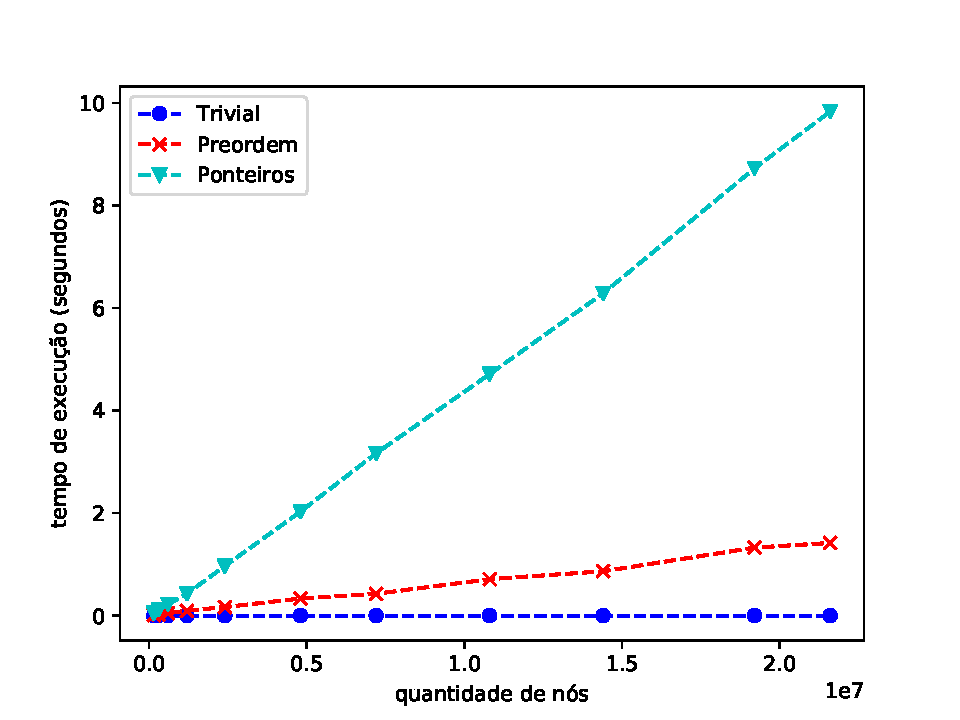
\includegraphics[scale=0.8]{preprocess_linear.pdf}
  \caption{Resultados para o preprocessamento de árvores lineares.}
\end{figure}

\newpage

\subsubsection{Árvores binárias}
Para estas árvores já é possível rodar o Algoritmo da Tabela para todos os tamanhos já
que sua complexidade de espaço agora é $\bigO(n \log n)$, sendo comparável com o
Algoritmo dos Ponteiros, que se mostrou menos eficiente. O Algoritmo da Preordem se tornou
ainda mais rápido, provavelmente por serem necessárias menos alocações de memória.

\begin{figure}
  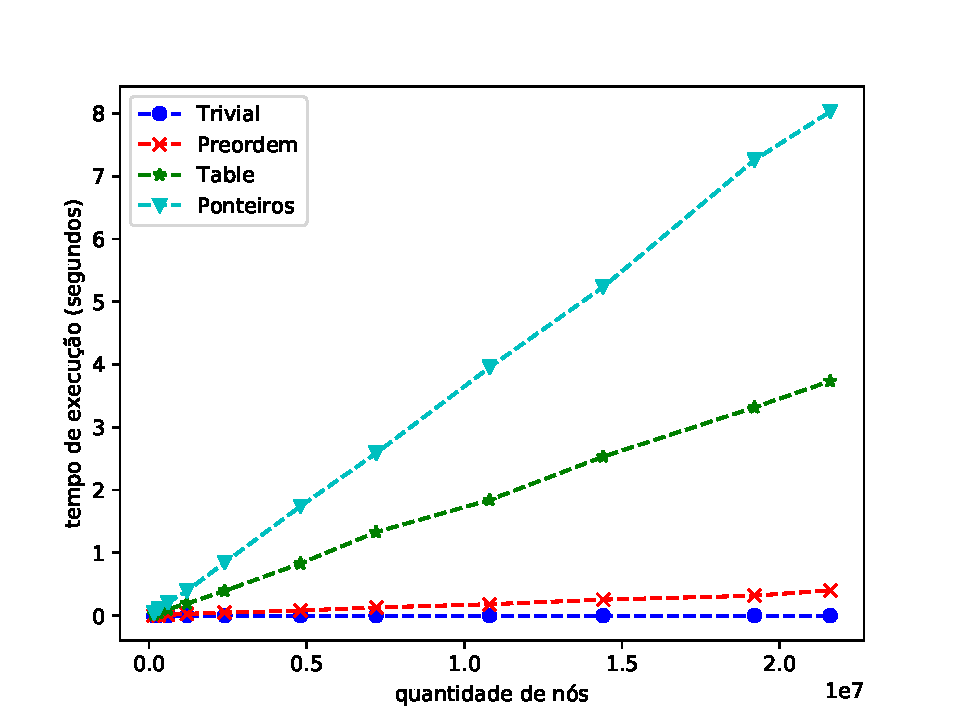
\includegraphics[scale=0.8]{preprocess_binary.pdf}
  \caption{Resultados para o preprocessamento de árvores binárias.}
\end{figure}

\subsubsection{Árvores quaternárias}
Para estas árvores é interessante notar que o desempenho do Algoritmo da Tabela foi
maior do que para árvores binárias e isso se deve à relação entre sua complexidade
de tempo e o fator de ramificação da árvore, já que esta é $\bigO(n \log_k n)$, onde
$k$ é o fator. O Algoritmo dos Ponteiros se manteve estável já que sua complexidade
não depende de $k$.

\begin{figure}[H]
  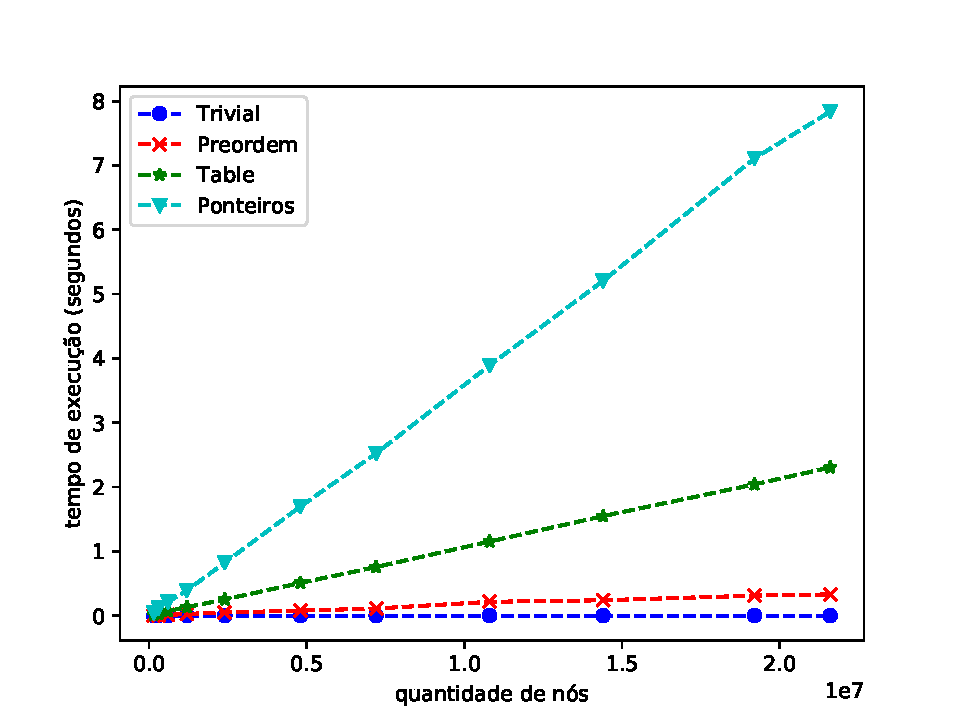
\includegraphics[scale=0.8]{preprocess_4ary.pdf}
  \caption{Resultados para o preprocessamento de árvores quaternárias.}
\end{figure}

\subsection{Consultas}

\subsubsection{Árvores lineares}
\subsubsection{Árvores binárias}

\begin{figure}[H]
  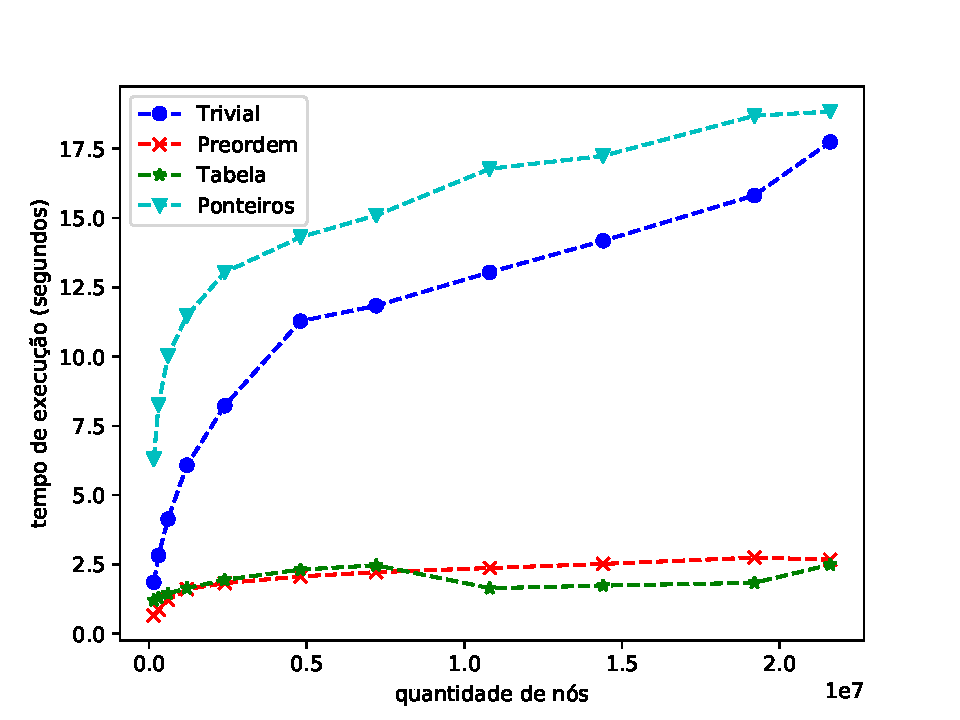
\includegraphics[scale=0.8]{query_binary.pdf}
  \caption{Resultados para as consultas em árvores binárias.}
\end{figure}

\subsubsection{Árvores quaternárias}

\begin{figure}[H]
  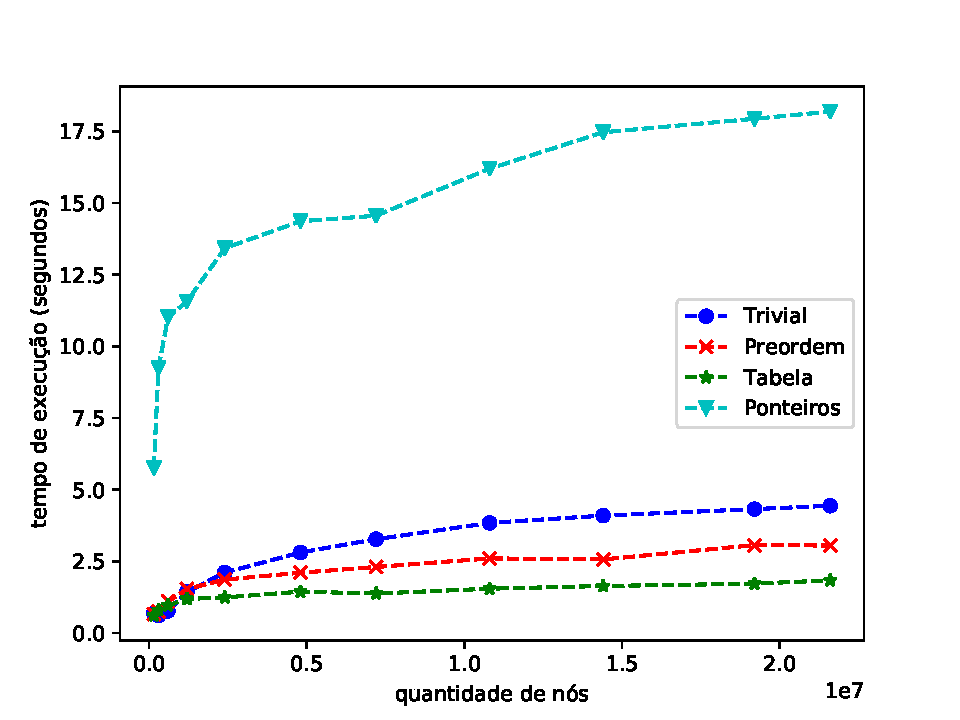
\includegraphics[scale=0.8]{query_4ary.pdf}
  \caption{Resultados para as consultas em árvores quaternárias.}
\end{figure}

\subsection{Conclusões}
Quase todos os algoritmos, exceto pelo algoritmo dos Ponteiros, se mostram mais
eficientes à medida que o fator de ramificação da árvore aumenta, já que isso causa
uma diminuição na sua profundidade esperada, que por sua vez tem relação direta com
a complexidade das implementações. É bastante interessante notar que implementações
simples como o algoritmo da Preordem e o da Tabela podem obter resultados muito
melhores do que outros mais complexos como o algoritmo dos Ponteiros. 
\par

%!TeX root=../tese.tex
%("dica" para o editor de texto: este arquivo é parte de um documento maior)
% para saber mais: https://tex.stackexchange.com/q/78101/183146

% Os capítulos de compõem a dissertação/tese, com numeração normal, podem
% ser inseridos diretamente aqui ou "puxados" de outros arquivos
%!TeX root=../tese.tex
%("dica" para o editor de texto: este arquivo é parte de um documento maior)
% para saber mais: https://tex.stackexchange.com/q/78101/183146

%% ------------------------------------------------------------------------- %%
\chapter{Uma introdução à Teoria dos Grafos}
\label{cap:introducao}

\section{As Pontes de Königsberg}

No século XVIII, a cidade de Königsberg, na Prússia (hoje Kaliningrado, na  atual 
Rússia) era um importante centro comercial devido à sua localização próxima ao rio,
que dividia a cidade em quatro regiões, interligadas por sete pontes.

\begin{figure}
  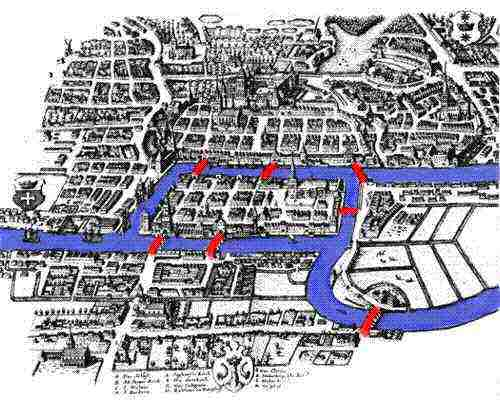
\includegraphics[scale=0.5]{Konigsberg.jpeg}
  \caption{A cidade de Königsberg e suas sete pontes}
\end{figure}

Segundo histórias, um passatempo de domingo dos cidadãos de Königsberg consistia em
passear por sua cidade, até que um dia surgiu um desafio: encontrar uma forma
de andar por todas as regiões passando por cada ponte apenas uma vez.

Nenhum habitante de Königsberg conseguiu encontrar a solução para este problema,
porém, o desafio chegou até um homem chamado Leonhard Euler, que apesar de julgar
o problema trivial, ficou intrigado, como citado em \citet{hopkins04:the}:

\begin{quotation}
  \emph{``This question is so banal, but seemed to me worthy of attention in that 
  [neither] geometry, nor algebra, nor even the art of counting was sufficient to
  solve it.''}
\end{quotation}

Euler provou que não era possível passar por toda a cidade de Königsberg sem passar
duas vezes pela mesma ponte, mas também resolveu o caso geral,
para qualquer número de regiões e qualquer número de pontes, dando assim origem
a um ramo da matemática que hoje chamamos de \textbf{Teoria dos Grafos}.

\section{Grafos}

Podemos definir um \textbf{Grafo} informalmente como um conjunto de entidades
conectadas entre si (ou não). Mais formalmente, podemos definir um grafo $G$ como um
par $(V, E)$ onde $V$ é um conjunto de \textbf{vértices} e $E$ um conjunto de
\textbf{arestas} entre os vértices tal que $E \subseteq \{ (u, v) \mid u, v \in V \}$.

As arestas de um grafo podem ter propriedades como direção e/ou algum valor
associado dependendo do contexto em que está sendo utilizado, frequentemente
possibilitando soluções elegantes e eficientes para os mais diversos problemas.

\begin{figure}
  \centering

  \begin{subfigure}{0.4\textwidth}
    \centering
    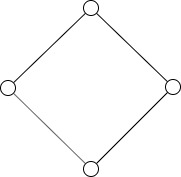
\includegraphics[width=.7\textwidth]{graph.jpg}
    \caption{Um grafo não dirigido.\label{fig:subfigures:a}}
  \end{subfigure}
  % ATENÇÃO: Se você deixar uma linha em branco entre as subfiguras,
  % LaTeX vai considerar que cada uma delas pertence a um "parágrafo"
  % diferente e, portanto, vai colocá-las em linhas separadas ao invés
  % de lado a lado.
  \begin{subfigure}{0.4\textwidth}
    \centering
    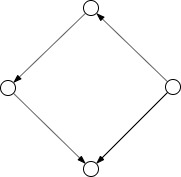
\includegraphics[width=.7\textwidth]{directed_graph.jpg}
    \caption{Um grafo dirigido.\label{fig:subfigures:b}}
  \end{subfigure}

  \begin{subfigure}{0.4\textwidth}
    \centering
    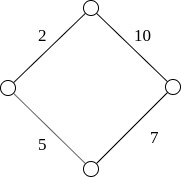
\includegraphics[width=.7\textwidth]{weighted_graph.jpg}
    \caption{Um grafo com valores nas arestas.\label{fig:subfigures:c}}
  \end{subfigure}
  \begin{subfigure}{0.4\textwidth}
    \centering
    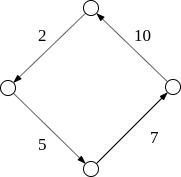
\includegraphics[width=.7\textwidth]{weighted_directed_graph.jpg}
    \caption{Um grafo dirigido com valores nas arestas.\label{fig:subfigures:d}}
  \end{subfigure}

  \caption{Exemplos de grafos.\label{fig:subfigures}}
\end{figure}

\section{Árvores}

\textbf{Árvores} são um subconjunto dos grafos de incrível importância para a
Ciência da Computação, sendo usadas nas mais diversas aplicações, desde a estrutura
de pastas de um sistema operacional até bancos de dados e processamento de
linguagem natural.

Diferente de outras estruturas como vetores, as árvores se organizam de forma
não linear, hierárquica. Os elementos de uma árvore são chamados de \textbf{nós} e
comumente um nó específico é elegido para ser a sua \textbf{raíz}. Cada nó pode
ter ligações com outros nós denominados \textbf{filhos}, que por sua vez podem
ter seus próprios filhos e assim sucessivamente até chegarmos em nós que não
possuem ligação com nenhum outro elemento; chamamos estes nós de \textbf{folhas}.

\begin{tikzpicture}[level/.style={sibling distance=60mm/#1}]
\node [circle,draw] (z){$n$}
  child {node [circle,draw] (a) {$\frac{n}{2}$}
    child {node [circle,draw] (b) {$\frac{n}{2^2}$}
      child {node {$\vdots$}
        child {node [circle,draw] (d) {$\frac{n}{2^k}$}}
        child {node [circle,draw] (e) {$\frac{n}{2^k}$}}
      } 
      child {node {$\vdots$}}
    }
    child {node [circle,draw] (g) {$\frac{n}{2^2}$}
      child {node {$\vdots$}}
      child {node {$\vdots$}}
    }
  }
  child {node [circle,draw] (j) {$\frac{n}{2}$}
    child {node [circle,draw] (k) {$\frac{n}{2^2}$}
      child {node {$\vdots$}}
      child {node {$\vdots$}}
    }
  child {node [circle,draw] (l) {$\frac{n}{2^2}$}
    child {node {$\vdots$}}
    child {node (c){$\vdots$}
      child {node [circle,draw] (o) {$\frac{n}{2^k}$}}
      child {node [circle,draw] (p) {$\frac{n}{2^k}$}
        child [grow=right] {node (q) {$=$} edge from parent[draw=none]
          child [grow=right] {node (q) {$O_{k = \lg n}(n)$} edge from parent[draw=none]
            child [grow=up] {node (r) {$\vdots$} edge from parent[draw=none]
              child [grow=up] {node (s) {$O_2(n)$} edge from parent[draw=none]
                child [grow=up] {node (t) {$O_1(n)$} edge from parent[draw=none]
                  child [grow=up] {node (u) {$O_0(n)$} edge from parent[draw=none]}
                }
              }
            }
            child [grow=down] {node (v) {$O(n \cdot \lg n)$}edge from parent[draw=none]}
          }
        }
      }
    }
  }
};
\path (a) -- (j) node [midway] {+};
\path (b) -- (g) node [midway] {+};
\path (k) -- (l) node [midway] {+};
\path (k) -- (g) node [midway] {+};
\path (d) -- (e) node [midway] {+};
\path (o) -- (p) node [midway] {+};
\path (o) -- (e) node (x) [midway] {$\cdots$}
  child [grow=down] {
    node (y) {$O\left(\displaystyle\sum_{i = 0}^k 2^i \cdot \frac{n}{2^i}\right)$}
    edge from parent[draw=none]
  };
\path (q) -- (r) node [midway] {+};
\path (s) -- (r) node [midway] {+};
\path (s) -- (t) node [midway] {+};
\path (s) -- (l) node [midway] {=};
\path (t) -- (u) node [midway] {+};
\path (z) -- (u) node [midway] {=};
\path (j) -- (t) node [midway] {=};
\path (y) -- (x) node [midway] {$\Downarrow$};
\path (v) -- (y)
  node (w) [midway] {$O\left(\displaystyle\sum_{i = 0}^k n\right) = O(k \cdot n)$};
\path (q) -- (v) node [midway] {=};
\path (e) -- (x) node [midway] {+};
\path (o) -- (x) node [midway] {+};
\path (y) -- (w) node [midway] {$=$};
\path (v) -- (w) node [midway] {$\Leftrightarrow$};
\path (r) -- (c) node [midway] {$\cdots$};
\end{tikzpicture}

Também definimos a \textbf{profundidade} de um nó como a quantidade
de arestas no caminho da raíz até ele. A raíz tem profundidade zero,
seus filhos profundidade um e assim sucessivamente.

\begin{figure}
  \centering
  \begin{tikzpicture}[
    level distance=1.5cm,
    level 1/.style={sibling distance=3cm},
    level 2/.style={sibling distance=1.5cm}]
    \node [circle, draw] {1}
      child {node [circle, draw] {2}
        child {node [circle, draw] {4}}
        child {node [circle, draw] {5}}
      }
      child {node [circle, draw] {3}
      child {node [circle, draw] {6}}
        child {node [circle, draw] {7}
        child [grow=right] {node (q) {$\qquad$} edge from parent[draw=none]
            child [grow=right] {node (q) {profundidade = 2} edge from parent[draw=none]
              child [grow=up] {node (r) {profundidade = 1} edge from parent[draw=none]
                child [grow=up] {node (s) {profundidade = 0} edge from parent[draw=none]
                }
              }
            }
          }
        }
      };
  \end{tikzpicture}
  \caption{O nó 1 é a raíz e tem como filhos os nós 2 e 3, cujos
  filhos são as folhas 4, 5 e 6, 7, respectivamente.}
  \end{figure}

\newpage

% Escrever bem é uma arte que exige muita técnica e dedicação e,
% consequentemente, há vários bons livros sobre como escrever uma boa
% dissertação ou tese. Um dos trabalhos pioneiros e mais conhecidos nesse
% sentido é o livro de
% %Umberto Eco~\cite{eco:09} % usando o estilo alpha
% Umberto~\citet{eco:09} % usando o estilo plainnat
% intitulado \emph{Como se faz uma tese}; é uma leitura bem interessante mas,
% como foi escrito em 1977 e é voltado para trabalhos de graduação na Itália,
% não se aplica tanto a nós.

% Sobre a escrita acadêmica em geral, John Carlis disponibilizou um texto curto
% e interessante~\citep{carlis:09} em que advoga a preparação de um único
% rascunho da tese antes da versão final. Mais importante que isso, no
% entanto, são os vários \textit{insights} dele sobre a escrita acadêmica.
% Dois outros bons livros sobre o tema são \emph{The Craft of Research}~\citep{craftresearch}
% e \emph{The Dissertation Journey}~\citep{dissertjourney}. Além disso, a USP
% tem uma compilação de normas relativas à produção de documentos
% acadêmicos~\citep{usp:guidelines} que pode ser utilizada como referência.

% Para a escrita de textos especificamente sobre Ciência da Computação, o
% livro de Justin Zobel, \emph{Writing for Computer Science}~\citep{zobel:04}
% é uma leitura obrigatória. O livro \emph{Metodologia de Pesquisa para
% Ciência da Computação} de
% %Raul Sidnei Wazlawick~\cite{waz:09} % usando o estilo alpha
% Raul Sidnei~\citet{waz:09} % usando o estilo plainnat
% também merece uma boa lida. Já para a área de Matemática, dois livros
% recomendados são o de Nicholas Higham, \emph{Handbook of Writing for
% Mathematical Sciences}~\citep{Higham:98} e o do criador do \TeX{}, Donald
% Knuth, juntamente com Tracy Larrabee e Paul Roberts, \emph{Mathematical
% Writing}~\citep{Knuth:96}.

% Apresentar os resultados de forma simples, clara e completa é uma tarefa que
% requer inspiração. Nesse sentido, o livro de
% %Edward Tufte~\cite{tufte01:visualDisplay}, % usando o estilo alpha
% Edward~\citet{tufte01:visualDisplay}, % usando o estilo plainnat
% \emph{The Visual Display of Quantitative Information}, serve de ajuda na
% criação de figuras que permitam entender e interpretar dados/resultados de forma
% eficiente.

% Além desse material, também vale muito a pena a leitura do trabalho de
% %Uri Alon \cite{alon09:how}, % usando o estilo alpha
% Uri \citet{alon09:how}, % usando o estilo plainnat
% no qual apresenta-se uma reflexão sobre a utilização da Lei de Pareto para
% tentar definir/escolher problemas para as diferentes fases da vida acadêmica.
% A direção dos novos passos para a continuidade da vida acadêmica deveria ser
% discutida com seu orientador.

% %% ------------------------------------------------------------------------- %%
% \section{Considerações de Estilo}
% \label{sec:consideracoes_preliminares}

% Normalmente, as citações não devem fazer parte da estrutura sintática da
% frase\footnote{E não se deve abusar das notas de rodapé.\index{Notas de rodapé}}.
% No entanto, usando referências em algum estilo autor-data (como o estilo
% plainnat do \LaTeX{}), é comum que o nome do autor faça parte da frase. Nesses
% casos, pode valer a pena mudar o formato da citação para não repetir o nome do
% autor; no \LaTeX{}, isso pode ser feito usando os comandos
% \textsf{\textbackslash{}citet}, \textsf{\textbackslash{}citep},
% \textsf{\textbackslash{}citeyear} etc. documentados no pacote
% natbib \citep{natbib}\index{natbib} (esses comandos são compatíveis com biblatex
% usando a opção \textsf{natbib=true}, ativada por padrão neste modelo). Em geral,
% portanto, as citações devem seguir estes exemplos:

% \small
% \begin{verbatim}
% Modos de citação:
% indesejável: [AF83] introduziu o algoritmo ótimo.
% indesejável: (Andrew e Foster, 1983) introduziram o algoritmo ótimo.
% certo: Andrew e Foster introduziram o algoritmo ótimo [AF83].
% certo: Andrew e Foster introduziram o algoritmo ótimo (Andrew e Foster, 1983).
% certo (\citet ou \citeyear): Andrew e Foster (1983) introduziram o algoritmo ótimo.
% \end{verbatim}
% \normalsize

% O uso desnecessário de termos em língua estrangeira deve ser evitado. No entanto,
% quando isso for necessário, os termos devem aparecer \textit{em itálico}.
% \index{Língua estrangeira}
% % index permite acrescentar um item no indice remissivo

% Uma prática recomendável na escrita de textos é descrever as
% legendas\index{Legendas} das figuras e tabelas em forma auto-contida: as
% legendas devem ser razoavelmente completas, de modo que o leitor possa entender
% a figura sem ler o texto onde a figura ou tabela é citada.\index{Floats}

% Sugerimos que você faça referências bibliográficas de forma similar aos
% estilos ``alpha'' (referências alfanuméricas) ou ``plainnat'' (referências
% por autor-data) de \LaTeX{}.  Se estiver usando natbib+bibtex\index{natbib}\index{bibtex},
% use os arquivos .bst ``alpha-ime.bst'' ou ``plainnat-ime.bst'', que são
% versões desses dois formatos traduzidas para o português. Se estiver usando
% biblatex\index{biblatex} (recomendado), escolha o estilo ``alphabetic''
% (que é um dos estilos padrão do biblatex) ou ``plainnat-ime''. O arquivo de
% exemplo inclui todas essas opções; basta des-comentar as linhas
% correspondentes e, se necessário, modificar o arquivo Makefile para chamar
% o bibtex\index{bibtex} ao invés do biber\index{biber} (este último é usado
% em conjunto com o biblatex).

% \section{Ferramentas Bibliográficas}

% Embora seja possível pesquisar por material acadêmico na Internet usando sistemas
% de busca ``comuns'', existem ferramentas dedicadas, como o \textsf{Google Scholar}\index{Google Scholar}
% (\url{scholar.google.com}). Você também pode querer usar o \textsf{Web of Science}\index{Web of Science}
% (\url{webofscience.com}) e o \textsf{Scopus}\index{Scopus} (\url{scopus.com}), que oferecem
% recursos sofisticados e limitam a busca a periódicos com boa reputação acadêmica.
% Essas duas plataformas não são gratuitas, mas os alunos da USP têm acesso a elas
% através da instituição. Ambas são capazes de exportar os dados para o formato .bib,
% usado pelo \LaTeX{}. Algumas editoras, como a ACM e a IEEE, também têm sistemas de
% busca bibliográfica.

% Apenas uma parte dos artigos acadêmicos de interesse está disponível livremente
% na Internet; os demais são restritos a assinantes. A CAPES assina um grande
% volume de publicações e disponibiliza o acesso a elas para diversas universidades
% brasileiras, entre elas a USP, através do seu portal de periódicos
% (\url{periodicos.capes.gov.br}). Existe uma extensão para os navegadores
% Chrome e Firefox (\url{www.infis.ufu.br/capes-periodicos}) que facilita o uso
% cotidiano do portal.

% Para manter um banco de dados organizado sobre artigos e outras fontes bibliográficas
% relevantes para sua pesquisa, é altamente recomendável que você use uma ferramenta
% como Zotero~(\url{zotero.org})\index{Zotero} ou
% Mendeley~(\url{mendeley.com})\index{Mendeley}. Ambas podem exportar seus dados no
% formato .bib, compatível com \LaTeX{}. Também existem três plataformas
% gratuitas que permitem a busca de referências acadêmicas já no formato .bib:

% \begin{itemize}
%   \item \emph{CiteULike}\index{CiteULike} (patrocinados por Springer): \url{www.citeulike.org}
%   \item Coleção de bibliografia em Ciência da Computação: \url{liinwww.ira.uka.de/bibliography}
%   \item Google acadêmico\index{Google Scholar} (habilitar bibtex nas preferências): \url{scholar.google.com}
% \end{itemize}

% Lamentavelmente, ainda não existe um mecanismo de verificação ou validação das
% informações nessas plataformas. Portanto, é fortemente sugerido validar todas
% as informações de tal forma que as entradas bib estejam corretas.

% De qualquer modo, tome muito cuidado na padronização das referências
% bibliográficas: ou considere TODOS os nomes dos autores por extenso, ou TODOS
% os nomes dos autores abreviados.  Evite misturas inapropriadas.

% \section{O Que o IME Espera}

% Ao terminar sua tese/dissertação, você deve entregar uma cópia dela para a
% CPG. Após a defesa, você tem 30 dias para revisar o texto e incorporar as
% sugestões da banca. Assim, há duas versões oficiais do documento: a versão
% original e a versão corrigida, o que deve ser indicado na folha de rosto.
% \index{Tese/Dissertação!versões}

% Fica a critério do aluno definir aspectos como o tamanho de fonte, margens,
% espaçamento, estilo de referências, cabeçalho, etc. considerando sempre o
% bom senso. A CPG, em reunião realizada em junho de 2007, aprovou que as
% teses/dissertações deverão seguir o formato padrão por ela
% definido\footnote{\url{www.ime.usp.br/dcc/pos/normas/tesesedissertacoes}}.
% Esse padrão refere-se aos itens que devem estar presentes nas teses/dissertações
% (e.g. capa, formato de rosto, sumário, etc.), e não à formatação do documento.
% Ele define itens obrigatórios e opcionais, conforme segue:\index{Formatação}
% \index{Tese/Dissertação!itens obrigatórios}
% \index{Tese/Dissertação!itens opcionais}

% \begin{itemize}
%   \item \textsc{Capa} (obrigatória)
%   \begin{itemize}
%     \item O IME usa uma capa padrão de cartolina para todas as
%     teses/dissertações.  Essa capa tem uma janela recortada por onde se
%     vê o título e o autor do trabalho e, portanto, a capa impressa do
%     trabalho deve incluir o título e o autor na posição correspondente da
%     página. Ela fica centralizada na página, tem 100mm de largura, 60mm de
%     altura e começa 47mm abaixo do topo da página.

%     \item O título da tese/dissertação deverá começar com letra maiúscula
%     e o resto deverá ser em minúsculas, salvo nomes próprios.

%     \item O nome do aluno(a) deverá ser completo e sem abreviaturas.

%     \item É preciso explicitar se é uma tese ou dissertação (para
%     obtenção do título de doutor, tese; para obtenção do título de
%     mestre, dissertação).

%     \item O nome do programa deve constar da capa (Matemática,
%     Matemática Aplicada, Estatística ou Ciência da Computação).

%     \item Também devem constar o nome completo do orientador e do
%     co-orientador, se houver.

%     \item Se o aluno recebeu bolsa, deve-se indicar a(s) agência(s).

%     \item É preciso informar o mês e ano do depósito ou da entrega da
%     versão corrigida.
%   \end{itemize}

%   \item \textsc{Folha de Rosto} (obrigatória, tanto para a versão
%   depositada quanto para a versão corrigida)
%   \begin{itemize}
%     \item o título da tese/dissertação deverá seguir o padrão da capa

%     \item deve informar se se trata da versão original ou da versão
%     corrigida; no segundo caso, deve também incluir os nomes
%     dos membros da banca.
%   \end{itemize}

%   \item \textsc{Agradecimentos} (opcional)

%   \item \textsc{Resumo}, em português (obrigatório)

%   \item \textsc{Abstract}, em inglês (obrigatório)

%   \item \textsc{Sumário} (obrigatório)

%   \item \textsc{Listas} (opcionais)
%   \begin{itemize}
%     \item Lista de Abreviaturas
%     \item Lista de Símbolos
%     \item Lista de Figuras
%     \item Lista de Tabelas
%   \end{itemize}

%   \item \textsc{Referências Bibliográficas} (obrigatório)

%   \item \textsc{Índice Remissivo} (opcional\footnote{O índice remissivo
%    pode ser muito útil para a banca; assim, embora seja um item opcional,
%    recomendamos que você o crie.})
% \end{itemize}

\par

%!TeX root=../tese.tex
%("dica" para o editor de texto: este arquivo é parte de um documento maior)
% para saber mais: https://tex.stackexchange.com/q/78101/183146

\chapter{O problema do Ancestral de Nível}
Uma consulta Ancestral de Nível $\mathrm{AN}(u, d)$ 

\newpage

\begin{program}   
      \lstinputlisting[
        language=pseudocode,
        style=pseudocode,
        style=wider,
        functions={},
        specialidentifiers={},
      ]
      {conteudo-exemplo/euclid.psc}
    
      \caption{Máximo divisor comum (arquivo importado).\label{prog:mdcinput}}
    \end{program}

\begin{program}
      \lstinputlisting[
        language=pseudocode,
        style=pseudocode,
        style=wider,
        functions={parent, depth},
        specialidentifiers={},
      ]
      {conteudo-exemplo/naive_query.psc}
    
      \caption{Naïve Algorithm query.\label{prog:mdcinput}}
    \end{program}

\newpage
%\chapter{Usando o \LaTeX{} e este modelo}

Não é necessário que o texto seja redigido usando \LaTeX{}, mas é fortemente
recomendado o uso dessa ferramenta, pois ela facilita diversas etapas do
trabalho e o resultado final é muito bom\footnote{O uso de um sistema de
controle de versões, como mercurial (\url{mercurial-scm.org}) ou git
(\url{git-scm.com}), também é altamente recomendado.}. Este modelo inclui
vários comentários explicativos e pacotes interessantes para auxiliá-lo com
ele, sendo composto dos arquivos principais de cada exemplo
(\texttt{tese.tex}, \texttt{artigo.tex},
\texttt{apresentacao.tex} e \texttt{poster.tex}) e de
vários arquivos auxiliares:

\begin{itemize}
  \item Arquivos com o conteúdo do trabalho:
  \begin{itemize}
    \item \texttt{conteudo/folhas-de-rosto.tex} (capa, dedicatória etc.)
    \item \texttt{conteudo/resumo-abstract.tex}
    \item \texttt{conteudo/capitulos.tex}, \texttt{conteudo/apendices.tex},
          \texttt{conteudo/anexos.tex} e demais arquivos carregados por eles
          (\texttt{XX-*.tex}, \texttt{apendice-pseudocodigo.tex}, \texttt{anexo-soft-livre.tex})
    \item \texttt{bibliografia.bib} (dados bibliográficos)
  \end{itemize}

  \item Arquivos com as \textit{packages} usadas e suas configurações (leia
        os comentários neles se quiser modificar algum aspecto do
        documento ou acrescentar alguma \textit{package}):
  \begin{itemize}
    \item \texttt{extras/basics.tex} (\textit{packages} e configurações essenciais),
          \texttt{extras/fonts.tex} (definição das fontes do documento) e
          \texttt{extras/floats.tex} (configurações e melhorias para \textit{floats})
    \item \texttt{extras/thesis-formatting.tex} (aparência: espaçamento, sumário etc.)
    \item \texttt{extras/index.tex} (configuração do índice remissivo)
    \item \texttt{extras/hyperlinks.tex} (configuração das referências cruzadas)
    \item \texttt{extras/source-code.tex} (exibição de código-fonte e pseudocódigo)
    \item \texttt{extras/utils.tex} (\textit{packages} adicionais diversas)
    \item \texttt{extras/bibconfig.tex} (configuração da bibliografia)
  \end{itemize}

  \item Outros arquivos auxiliares (geralmente não precisam ser editados):
  \begin{itemize}
    \item \texttt{extras/imeusp-capa.sty} (formatação da capa e demais páginas iniciais)
    \item \texttt{extras/imeusp-headers.sty} (formatação dos cabeçalhos)
    \item \texttt{extras/lstpseudocode.sty} (suporte a pseudocódigo com \textsf{listings})
    \item \texttt{extras/annex.sty} (permite adicionar anexos) e
          \texttt{extras/appendixlabel.sty} (melhora a lista de
          apêndices/anexos no sumário)
    \item \texttt{extras/beamer*.sty} (\textit{layouts} e cores para
          apresentações e \textit{posters})
    \item \texttt{extras/plainnat-ime.*} (estilo plainnat para bibliografias)\index{biblatex}
    \item \texttt{extras/alpha-ime.bst} (estilo alpha para bibliografias com
          bibtex)\index{bibtex}
    \item \texttt{extras/natbib-ime.sty} (tradução da \textit{package}
          padrão natbib)\index{natbib}
    \item \texttt{hyperxindy.xdy} (configuração para xindy) e
          \texttt{mkidxhead.ist} (configuração para makeindex)
    \item \texttt{latexmkrc} e \texttt{Makefile} (automatizam a geração do
          documento com os comandos \textsf{latexmk} e \textsf{make} respectivamente)
  \end{itemize}
\end{itemize}

Para compilar o documento, basta executar o comando \textsf{latexmk} (ou
\textsf{make})\footnote{Você também pode usar \textsf{latexmk poster},
\textsf{make apresentacao} etc.}. Talvez seu editor ofereça uma
opção de menu para compilar o documento, mas ele provavelmente depende do
\textsf{latexmk} para isso. \LaTeX{} gera diversos arquivos auxiliares
durante a compilação que, em algumas raras situações, podem ficar
inconsistentes (causando erros de compilação ou erros no PDF gerado, como
referências faltando ou numeração de páginas incorreta no sumário). Nesse
caso, é só usar o comando \textsf{latexmk -C} (ou \textsf{make clean}),
que apaga todos os arquivos auxiliares gerados, e em seguida rodar
\textsf{latexmk} (ou \textsf{make}) novamente.

\section{Instalação do \LaTeX{}}
\label{sec:install}

\enlargethispage{-.5\baselineskip}

\LaTeX{} é, na verdade, um conjunto de programas. Ao invés de procurar e
baixar cada um deles, o mais comum é baixar um pacote com todos eles juntos.
Há dois pacotes desse tipo disponíveis: MiK\TeX{} (\url{miktex.org}) e
\TeX{}Live (\url{www.tug.org/texlive}). Ambos funcionam em Linux, Windows e
MacOS X. Em Linux, \TeX{}Live costuma estar disponível para instalação junto
com os demais opcionais do sistema. Em MacOS X, o mais popular é o Mac\TeX{}
(\url{www.tug.org/mactex/}), a versão do \TeX{}Live para MacOS X.  Em Windows,
o mais comumente usado é o MiK\TeX{}.

Por padrão, eles não instalam tudo que está disponível, mas sim apenas os
componentes mais usados, e oferecem um gestor de pacotes que permite adicionar
outros. Embora uma instalação completa do \LaTeX{} seja relativamente grande
(perto de 5GB), em geral vale a pena instalar a maior parte dos pacotes. Se
você preferir uma instalação mais ``enxuta'', não deixe de incluir todos os
pacotes necessários para este modelo, como indicado no arquivo README.md.

Também é muito importante ter o \textsf{latexmk} (ou o \textsf{make}). No Linux,
a instalação é similar à de outros programas. No MacOS X e no Windows,
\textsf{latexmk} pode ser instalado pelo gestor de pacotes do MiK\TeX{} ou
\TeX{}Live. Observe que ele depende da linguagem \textsf{perl}, que precisa ser
instalada à parte no Windows (\url{www.perl.org/get.html}).

\section{Documentação sobre \LaTeX}
\label{sec:docs}

Existem diversos bons livros sobre \LaTeX{} (embora em geral um tanto
antigos), dos quais destacamos dois:

\begin{enumerate}

  \item A quarta edição de ``A Guide to \LaTeX'', de Helmut Kopka e
        Patrick W. Daly (publicada em 2003), além de uma ótima
        introdução, aborda vários tópicos relativamente avançados e
        úteis\footnote{Um dos autores disponibiliza uma versão não-final
        em \url{www2.mps.mpg.de/homes/daly/GTL/gtl_20030512.pdf}.}.
  \item A segunda edição de ``The \LaTeX{} Companion'' (publicada em
        2004) é um livro quase obrigatório, pois discute em detalhes
        praticamente todos os recursos e \textit{packages} importantes
        de \LaTeX{}, servindo tanto para o aprendizado quanto como
        material de referência.

\end{enumerate}

\enlargethispage{-.5\baselineskip}

Além de livros, há muito material sobre \LaTeX{} na Internet, mas também há
muita informação obsoleta. Em particular, você pode ignorar explicações sobre
como converter arquivos no formato DVI gerados por \LaTeX{} em PDF: versões
modernas de \LaTeX{} geram arquivos PDF diretamente. Quanto a imagens, os
formatos de arquivo PS/EPS (PostScript e Encapsulated PostScript) não são mais
aceitos; hoje em dia \LaTeX{} trabalha com arquivos de imagem nos formatos PDF,
PNG e JPEG. Finalmente, recursos gráficos não usam mais \textit{packages} como
\textsf{pstricks}, \textsf{eepic} ou outras tradicionalmente citadas; ao invés
disso, \textsf{PGF/TikZ} é a ferramenta mais comum.

Dentre o material online, o conteúdo em \url{overleaf.com/learn} é excelente,
incluindo um rápido tutorial (de escopo similar ao Capítulo~\ref{chap:tutorial}
deste modelo) e várias páginas sobre como utilizar recursos específicos. Um
tutorial bastante abrangente e detalhado está disponível em
\url{tug.org/twg/mactex/tutorials/ltxprimer-1.0.pdf} (há outros, como
\url{tug.org/tutorials/tugindia},
\url{www.maths.tcd.ie/~dwilkins/LaTeXPrimer/GSWLaTeX.pdf} e
\url{www.andy-roberts.net/writing/latex}). Em português, você pode consultar
\url{polignu.org/sites/polignu.org/files/latex/latex-fflch.pdf} e
\url{git.febrace.org.br/material-latex/material-latex} (este precisa ser
baixado e compilado). O sítio \url{tex.stackexchange.com} é
um fórum de perguntas e respostas sobre \LaTeX{} muito útil, pois os
principais desenvolvedores do sistema participam das discussões, e o sítio
\url{texfaq.org} é bastante abrangente e atualizado. O canal
\url{youtube.com/c/anteroneves} tem vários vídeos instrutivos em português.

Como dito anteriormente, \LaTeX{} é, na verdade, um conjunto de programas e,
normalmente, instalamos pacotes pré-prontos com todos eles. Esses pacotes (em
geral, \TeX{}Live e MiK\TeX{}) contém também a documentação das
\textit{packages} incluídas: Basta digitar \textsf{texdoc nome-da-package}
(\TeX{}Live) ou \textsf{mthelp nome-da-package} (MiK\TeX{}) para ter acesso à
documentação correspondente. \textsf{texdoc/mthelp} incluem também alguns
tutoriais e textos introdutórios, como ``The Not So Short Introduction to
\LaTeXe{}'' (\textsf{texdoc lshort-eng}; há uma versão em português, mas não
está em dia com o original), ``Getting up and running with \AmS-\LaTeX{}''
(\textsf{texdoc amshelp}) e ``A Simplified Introduction to \LaTeX{}''
(\textsf{texdoc simplified-intro}). Versões recentes do \LaTeX{} incluem
também o ``\LaTeXe{} via exemplos'' (\textsf{texdoc latex-via-exemplos}),
em português. O sítio \url{texdoc.net} oferece acesso online a essa mesma
documentação de maneira organizada e o sítio \url{ctan.org} é o
repositório semi-oficial das \textit{packages} \LaTeX{} e sua documentação.

A documentação de referência de \LaTeX{} pode ser acessada com \textsf{texdoc
latex2e} e \textsf{texdoc source2e}; a documentação de referência das classes
padrão (\textsf{article, book etc}), por sua vez, com \textsf{texdoc classes}.
Você normalmente não vai usá-las, mas elas podem servir para esclarecer algum
detalhe. \textsf{texdoc clsguide} é um guia para a criação de novas classes e
\textit{packages}, e \textsf{texdoc fntguide} explica como funciona a gestão
de fontes de \LaTeX{} (mas note que \LuaLaTeX{} e \XeLaTeX{} usam outro
mecanismo). Você pode ver exemplos de fontes disponíveis para \LaTeX{} em
\url{tug.org/FontCatalogue}.

Quando você se tornar um usuário avançado, pode se interessar em conhecer
melhor a linguagem \TeX{}, que está na base do \LaTeX{}. ``The \TeX{} book'',
de Donald Knuth, é amplamente recomendado, mas há três livros completos a
respeito que são instalados com \LaTeX{}: ``A gentle introduction to \TeX{}''
(\textsf{texdoc gentle}), ``\TeX{} for the impatient'' (\textsf{texdoc
impatient}) e ``\TeX{} by topic'' (\textsf{texdoc texbytopic}).

\par

%!TeX root=../tese.tex
%("dica" para o editor de texto: este arquivo é parte de um documento maior)
% para saber mais: https://tex.stackexchange.com/q/78101/183146

% Vamos definir alguns comandos auxiliares para facilitar.

% "textbackslash" é muito comprido.
\newcommand{\sla}{\textbackslash}

% Vamos escrever comandos (como "make" ou "itemize") com formatação especial.
\newcommand{\cmd}[1]{\textsf{#1}}

% Idem para packages; aqui estamos usando a mesma formatação de \cmd,
% mas poderíamos escolher outra.
\newcommand{\pkg}[1]{\textsf{#1}}

% A maioria dos comandos LaTeX começa com "\"; vamos criar um
% comando que já coloca essa barra e formata com "\cmd".
\newcommand{\ltxcmd}[1]{\cmd{\sla{}#1}}

\chapter{O Problema do Ancestral de Nível e Implementações}
\label{chap:implementacoes}

\section{Definição do problema}
O problema do \textbf{Ancestral de Nível} é um problema fundamental de árvores que pode
ser definido da seguinte forma: Dada uma árvore enraizada $T$ com $n$ nós, para
consultas $\mathrm{AN}(u, d)$ onde $u$ é um nó de $T$ e $d$ um número inteiro,
encontre o ancestral de profundidade $d$ de $u$ otimizando tanto o tempo de
preprocessamento quanto o de resposta às consultas.

\tikzset{
  treenode/.style = {align=center, minimum size=7mm, inner sep=0pt, text centered},
  arn_n/.style = {treenode, circle, white, font=\bfseries, draw=black,
    fill=black, text width=1.5em},% arbre rouge noir, noeud noir
  arn_r/.style = {treenode, circle, red, draw=red, 
    text width=1.5em, very thick},% arbre rouge noir, noeud rouge
  arn_x/.style = {treenode, circle, draw=black, minimum size=7mm}% arbre rouge noir, nil
}

\begin{figure}[H]
    \begin{tikzpicture}[scale=0.7,
      level distance=1.5cm,
      level 1/.style={sibling distance=6cm},
      level 2/.style={sibling distance=3cm},
      level 3/.style={sibling distance=1.5cm}]
      \node [arn_x] {0}
        child {node [arn_x] {1}
          child {node [arn_x] {3}
            child {node [arn_x] {7}}
            child {node [arn_x] {8}}
          }
          child {node [arn_x] {4}
            child {node [arn_x] {9}}
            child {node [arn_x] {10}}
          }
        }
        child {node [arn_r] {2}
          child {node [arn_x] {5}
            child {node [arn_x] {11}}
            child {node [arn_x] {12}}
          }
          child {node [arn_x] {6}
              child {node [arn_n] {13}}
              child {node [arn_x] {14}}
          }
        };
    \end{tikzpicture}
    \caption[Exemplo de consulta de Ancestral de Nível]
    {Exemplo de consulta AN(13, 1) = 2.}
  \end{figure}

  \begin{figure}[H]
    \begin{tikzpicture}[scale=0.7,
        level distance=1.5cm,
        level 1/.style={sibling distance=6cm},
        level 2/.style={sibling distance=3cm},
        level 3/.style={sibling distance=1.5cm}]
        \node [arn_x] {0}
          child {node [arn_x] {1}
            child {node [arn_x] {3}
              child {node [arn_x] {7}}
              child {node [arn_x] {8}}
            }
            child {node [arn_r] {4}
              child {node [arn_n] {9}}
              child {node [arn_x] {10}}
            }
          }
          child {node [arn_x] {2}
            child {node [arn_x] {5}
              child {node [arn_x] {11}}
              child {node [arn_x] {12}}
            }
            child {node [arn_x] {6}
                child {node [arn_x] {13}}
                child {node [arn_x] {14}}
            }
          };
      \end{tikzpicture}
      \caption[Exemplo de consulta de Ancestral de Nível]
      {Exemplo de consulta AN(9, 2) = 4.}
    \end{figure}

Existem diversas soluções para tal problema, de diferentes níveis de complexidade e
com performances teoricamente diferentes. Em particular, por exemplo, é possível
realizar as consultas de forma trivial sem qualquer tipo de preprocessamento ou também
preprocessar todas as possíveis consultas para que possam então ser respondidas
rapidamente.

Em \citet{Bender2002TheLA}, \citet{LAInPractice} e \citet{menghani2019simple} são
discutidas algumas soluções, incluindo as que serão implementadas e testadas neste
trabalho. Em particular, preferi testar soluções que fossem razoavelmente simples
de serem implementadas, até mesmo para mostrar que estas são muitas vezes bastante
suficientes.

Como motivação para o estudo deste problema, vale lembrar que o Ancestral de Nível
aparece como parte de problemas mais complexos como árvores ordinais espaço-eficientes
como descrito em \citet{Geary:2006:SOT:1198513.1198516} que podem ser usadas na
representação de documentos XML que suportam consultas XPath. Além disso, são usadas
em \citet{Sadakane:2006:SSD:1109557.1109693} para implementar estruturas de dados
comprimidas e também em \citet{Yuan:2009:EDS:1514894.1514908} para consultas agregadas
em árvores. Por último, vemos aplicações até mesmo no campo de \textit{hashing} em
strings, como dito em \citet{10.1007/3-540-61258-0_11}.

\section{Implementações}

Todas as implementações assumem a mesma implementação de árvore onde é
guardada apenas sua raíz e cada nó contém um vetor de ponteiros para seus
filhos. Para facilitar as implementações, ao construir a árvore é feita uma
busca em profundidade para preencher vetores que servirão como funções globais
\texttt{pai()} e \texttt{profundidade()}.

\begin{program}[H]
  \lstinputlisting[
    language=pseudocode,
    style=pseudocode,
    style=wider,
    functions={travessia},
    specialidentifiers={global},
  ]
  {conteudo-exemplo/tree.psc}

  \caption{Criação da árvore.\label{prog:tree}}
\end{program}

Estamos interessados em analisar, para cada algoritmo, tanto sua complexidade de
tempo de execução quanto a de espaço adicional, também levando em consideração quão
simples é sua implementação.

Para tornar a discussão da complexidade de tempo mais clara, vamos dizer que se um
algoritmo tem complexidade de tempo $\langle f(x), g(x) \rangle$, a complexidade de
seu preprocessamento é $f(x)$ e de suas consultas é $g(x)$.

\subsection{Algoritmo Trivial}

O primeiro algoritmo a ser estudado é um em que simplesmente não há
nenhum preprocessamento e, para cada consulta, apenas subimos pelos pais a
partir do nó em questão até encontrarmos seu ancestral com profundidade igual
à profundidade requisitada.

%\subsection*{Preprocessamento}
Para esta implementação, o tempo de execução de seu preprocessamento não depende do
tamanho da árvore e também não utiliza nenhuma memória adicional, portanto o
preprocessamento do Algoritmo Trivial tem complexidade $\bigO(1)$ tanto para tempo
quanto espaço.

%\subsection*{Consultas}

No que diz respeito a cada consulta, precisamos chamar a função $pai()$
partindo do nó inicial até chegar no nó com a profundidade desejada.
Essa quantidade é exatamente a diferença entre esta profundidade e a
profundidade do nó inicial.

\begin{program}[]
  \lstinputlisting[
    language=pseudocode,
    style=pseudocode,
    style=wider,
    functions={pai, profundidade},
    specialidentifiers={},
  ]
  {conteudo-exemplo/naive_query.psc}

  \caption{Consulta do Algoritmo Trivial.\label{prog:naivequery}}
\end{program}

A consulta mais lenta para uma árvore qualquer é uma que parte do nó mais profundo
e precisa subir até a raíz, levando tempo $\bigO(d)$, onde $d$ é a profundidade
da árvore. No pior caso isso é equivalente a $\bigO(n)$ onde $n$ é a quantidade
de nós e para uma árvore balanceada cujos nós tem $k$ filhos, é equivalente a
$\bigO(\log_k n)$, fazendo com que a performance da consulta seja muito dependente da
forma da árvore.

Após essa análise, podemos concluir que o Algoritmo Trivial tem complexidade de tempo
$\langle \bigO(1), \bigO(d) \rangle$ e $\bigO(1)$ de espaço adicional, sendo
particularmente eficiente para árvores balanceadas e com fator de ramificação maior.


\subsection{Algoritmo da Tabela}
Ao contrário do algoritmo trivial, a ideia é precalcular o resultado de todas
as consultas possíveis durante a fase de preprocessamento para otimizar o
desempenho da fase de consultas.

Cada nó $u$ tem associado a si $profundidade(u) + 1$ possíveis consultas. Assim, para uma
árvore com $n$ nós, existem $n + \sum_{i=0}^{n-1} profundidade(i) = \bigO(nd)$ consultas, onde $d$ é a profundidade da árvore.
O preprocessamento se dá de maneira simples, preenchendo uma tabela de tamanho
$\bigO(nd)$ com dois laços encadeados, utilizando a função $pai()$ para subir a partir
de cada nó até a raíz e salvar a resposta para cada profundidade.

\begin{program}[]
  \lstinputlisting[
    language=pseudocode,
    style=pseudocode,
    style=wider,
    functions={pai, profundidade},
    specialidentifiers={},
  ]
  {conteudo-exemplo/table_preprocessing.psc}

  \caption{Preprocessamento do Algoritmo da Tabela.\label{prog:tableproc}}
\end{program}

Com a tabela devidamente preenchida, as consultas se tornam tão simples quanto acessar
a sua entrada correspondente, ou seja, a resposta da consulta que pede pelo ancestral
do nó $u$ com profundidade $p$ é dada por $tabela[u][p]$. 

\begin{program}[h!]
  \lstinputlisting[
    language=pseudocode,
    style=pseudocode,
    style=wider,
    functions={pai, profundidade},
    specialidentifiers={},
  ]
  {conteudo-exemplo/table_query.psc}

  \caption{Consulta do Algoritmo da Tabela.\label{prog:tablequery}}
\end{program}

A complexidade de espaço e de tempo do preprocessamento dependem fortemente da forma da
árvore, podendo ser $\bigO(n^2)$ no caso de uma árvore linear e para o caso de uma
árvore $k$-ária balanceada é $\bigO(n \log_k n)$, muito mais eficiente. Já a consulta
é feita em tempo $\bigO(1)$, sem uso de espaço adicional. Assim, o Algoritmo da Tabela
tem complexidade de tempo $\langle \bigO(nd), \bigO(1) \rangle$ e $\bigO(nd)$ de espaço,
sendo uma boa opção para casos de árvores balanceadas em que o preprocessamento se torna
barato frente à quantidade de consultas que serão feitas e o espaço utilizado não é
uma restrição.


\subsection{Algoritmo dos Ponteiros}
Essa é possivelmente a solução mais complexa que vamos analisar

\begin{program}[h!]
  \lstinputlisting[
    language=pseudocode,
    style=pseudocode,
    style=wider,
    functions={dfs, filhos, insere},
    specialidentifiers={global},
  ]
  {conteudo-exemplo/jump_preprocess.psc}

  \caption{Preprocessamento do Algoritmo da Preordem.\label{prog:preorderproc}}
\end{program}

\subsection{Algoritmo da Preordem}
O último algoritmo faz uso das propriedades da preordem de uma árvore para trazer uma
solução mais eficiente. Enquanto é feita a travessia da árvore cada nó é associado à
seu índice na preordem, que é inserido numa lista de nós de sua respectiva profundidade.

\begin{figure}
  \centering
  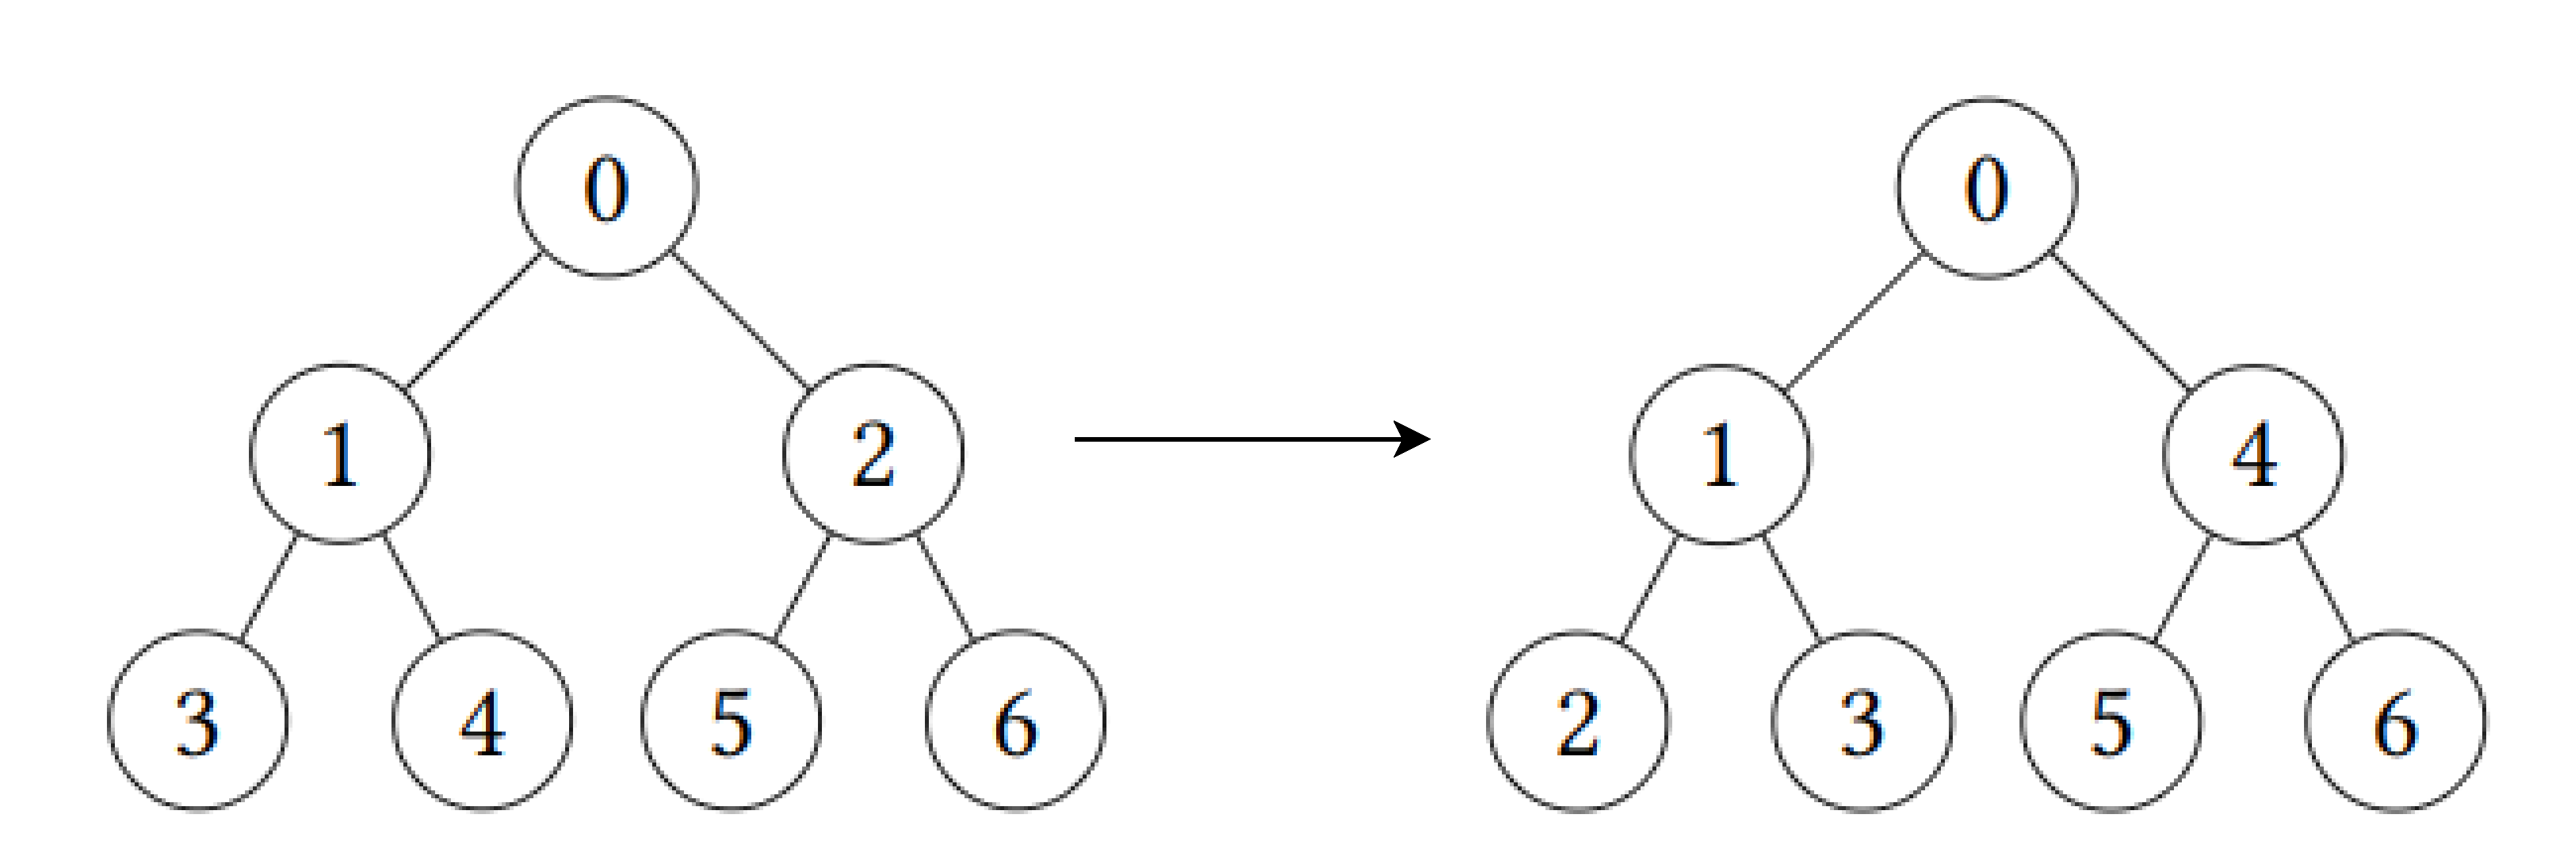
\includegraphics[scale=0.18]{preordertransformation.pdf}
  \caption{Associação entre os índices originais e os índices da preordem.}
\end{figure}

\begin{table}[]
  \begin{tabular}{llllll}
  \cline{3-3}
  profundidade 0: & \multicolumn{1}{l|}{} & \multicolumn{1}{l|}{0} &                        &                        &                        \\ \cline{3-3}
                  &                       &                        &                        &                        &                        \\ \cline{3-4}
  profundidade 1: & \multicolumn{1}{l|}{} & \multicolumn{1}{l|}{1} & \multicolumn{1}{l|}{4} &                        &                        \\ \cline{3-4}
                  &                       &                        &                        &                        &                        \\ \cline{3-6} 
  profundidade 2: & \multicolumn{1}{l|}{} & \multicolumn{1}{l|}{2} & \multicolumn{1}{l|}{3} & \multicolumn{1}{l|}{5} & \multicolumn{1}{l|}{6} \\ \cline{3-6} 
  \end{tabular}
  \caption[Vetores contendo os nós processados em cada nível.]
  {Vetores contendo os nós processados em cada nível. Os índices são referentes à preordem.}
\end{table}

Para tal, a ideia é guardar a ordem em que os nós de cada nível
foram visitados durante a travessia em preordem em vetores e então uma consulta se
resume a procurar o ancestral do nó inicial que está no vetor correspondente à
profundidade buscada.

\begin{program}[h!]
  \lstinputlisting[
    language=pseudocode,
    style=pseudocode,
    style=wider,
    functions={dfs, filhos, insere},
    specialidentifiers={global},
  ]
  {conteudo-exemplo/preorder_preprocess.psc}

  \caption{Preprocessamento do Algoritmo da Preordem.\label{prog:preorderproc}}
\end{program}

Para entendermos o funcionamento do algoritmo para as consultas, primeiro precisamos
nos convencer de que, se um nó $v$ é ancestral de $u$, então $preordem(v) < preordem(u)$,
onde $preordem(x)$ é o índice associado à posição de $x$ na travessia em preordem, já
que sempre descobrimos os filhos de um nó depois dele próprio. Além disso, no caso em
que existam vários nós em determinada profundidade, o ancestral que buscamos é aquele
cujo índice na preordem é o mais próximo do índice do nó inicial, porém ainda menor
que tal.

\begin{program}[]
  \lstinputlisting[
    language=pseudocode,
    style=pseudocode,
    style=wider,
    functions={upper_bound},
    specialidentifiers={},
  ]
  {conteudo-exemplo/preorder_query.psc}

  \caption{Consulta do Algoritmo da Preordem.\label{prog:preorderquery}}
\end{program}

\section{Considerações gerais}
No próximo capítulo estaremos interessados em avaliar a performance de cada algoritmo
para alguns casos de teste, levando em consideração o preprocessamento necessário,
a realização de consultas e a quantidade de memória utilizada.

Entretanto, analisando as tabelas ~\ref{tab:complexidadetempo},
~\ref{tab:complexidadeespaco} podemos perceber de imediato que restringir a entrada
para árvores balanceadas permite até mesmo que os algoritmos mais simples apresentem
complexidades boas, sendo ótimas opções levando em consideração também a dificuldade
de implementação de cada algoritmo.

\begin{table}[]
  \begin{tabular}{|c|l|l|l|}
  \hline
            & Linear                                       & Binária                                      & k-ária                                       \\ \hline
  Trivial   & $\langle \bigO(1), \bigO(n) \rangle$                 & $\langle \bigO(1), \bigO(\log_2 n) \rangle$          & $\langle \bigO(1), \bigO(\log_k n) \rangle$          \\ \hline
  Tabela    & $\langle \bigO(n^2), \bigO(1) \rangle$               & $\langle \bigO(n \log_2 n), \bigO(1) \rangle$        & $\langle \bigO(n \log_k n), \bigO(1) \rangle$        \\ \hline
  Ponteiros & $\langle \bigO(n \log_2 n), \bigO(\log_2 n) \rangle$ & $\langle \bigO(n \log_2 n), \bigO(\log_2 n) \rangle$ & $\langle \bigO(n \log_2 n), \bigO(\log_2 n) \rangle$ \\ \hline
  Preordem  & $\langle \bigO(n), \bigO(1) \rangle$                 & $\langle \bigO(n), \bigO(\log_2 n) \rangle$          & $\langle \bigO(n), \bigO(\log_2 n) \rangle$          \\ \hline
  \end{tabular}
  \caption{Comparação da complexidade de tempo dos algoritmos.\label{tab:complexidadetempo}}
  \end{table}

  \begin{table}[]
    \begin{tabular}{|c|l|l|l|}
    \hline
              & Linear              & Binária             & k-ária              \\ \hline
    Trivial   & $\bigO(1)$          & $\bigO(1)$              & $\bigO(1)$              \\ \hline
    Tabela    & $\bigO(n^2)$        & $\bigO(n \log_2 n)$     & $\bigO(n \log_k n)$ \\ \hline
    Ponteiros & $\bigO(n \log_2 n)$ & $\bigO(n \log_2 n)$ & $\bigO(n \log_2 n)$ \\ \hline
    Preordem  & $\bigO(n)$          & $\bigO(n)$          & $\bigO(n)$          \\ \hline
    \end{tabular}
    \caption{Comparação da complexidade de espaço dos algoritmos.\label{tab:complexidadeespaco}}
    \end{table}

\par

%!TeX root=../tese.tex
%("dica" para o editor de texto: este arquivo é parte de um documento maior)
% para saber mais: https://tex.stackexchange.com/q/78101/183146

\chapter{Benchmarks}
\label{chap:benchmarks}

\section{Metodologia}
Os algoritmos foram implementados na linguagem C++ usando apenas as bibliotecas
padrão e a STL. Todos os programas foram compilados com a versão 7.4.0 do
compilador g++, num computador que possui um processador Intel Core i5-8250U
com clock base de 1.60GHz e turbo boost até 3.40GHz em uma única thread. As medições
de tempo foram feitas com o \texttt{steady\_clock} da biblioteca \texttt{<chrono>},
utilizando uma precisão de nanosegundos, tomando o devido cuidado de cronometrar apenas
as partes relevantes do código. Todos os programas foram compilados com a flag
\texttt{-O2} para permitir otimizações por parte do compilador.

Para cada algoritmo apresentado neste trabalho, foram medidos os tempos de execução tanto
da parte de preprocessamento quanto da parte de consultas, separadamente. Cada teste
também foi realizado com árvores lineares, binárias e quaternárias para evidenciar 
possíveis diferenças de performance de acordo com o formato da árvore.

Todas as árvores geradas para fins destes testes são completas (portanto balanceadas) 
e seus tamanhos variaram entre 150K e 21.6M. Tanto os testes de preprocessamento quanto
os de consultas foram executados dez vezes com cada tamanho de árvore para tomar então
suas médias como resultado. 

Os testes de preprocessamento consistem em um programa que cria uma árvore completa
com a quantidade de nós e o fator de ramificação desejados e então cria um objeto da
classe associada ao algoritmo a ser testado, o que equivale à fase de preprocessar a
árvore de entrada. Já os testes de consultas consistem em um programa que cria também
uma árvore completa com os mesmos parâmetros e então executam um conjunto de 10M de
consultas gerado previamente. Estes arquivos foram gerados aleatoriamente de forma que
toda consulta seja composta por um nó válido (entre 0 e $N-1$) onde $N$ é o tamanho do
experimento e uma profundidade válida (entre 0 e $profundidade(u)$), onde $u$ é o nó
da consulta.

\section{Análise dos resultados}
As árvores que surgiriam em aplicações reais possivelmente não seriam exatamente como
as árvores aqui testadas, que são todas completas, porém ainda podemos ter uma boa
noção de como as diferentes implementações se comportam no pior caso possível e em casos
mais favoráveis.

\subsection{Preprocessamento}

\subsubsection{Árvores lineares}
A primeira coisa a ser notada é que, para árvores lineares, o Algoritmo da Tabela mal
pode ser comparado com os outros, já que para este caso sua complexidade de espaço
de preprocessamento é $\bigO(n^2)$, se tornando impossível manter o programa na memória
até mesmo para o menor tamanho de árvore, 150K. Apesar disso, não é interessante
diminuir as árvores para que os testes não se tornem facilmente influenciáveis por
fatores do sistema como trocas de contexto, por exemplo.

Como esperado, o algoritmo da Preordem leva uma vantagem grande sobre o algoritmo dos
Ponteiros devido à diferença de complexidade entre eles e o Trivial se mantém
essencialmente constante, a menos de pequenas variações.

\begin{figure}
  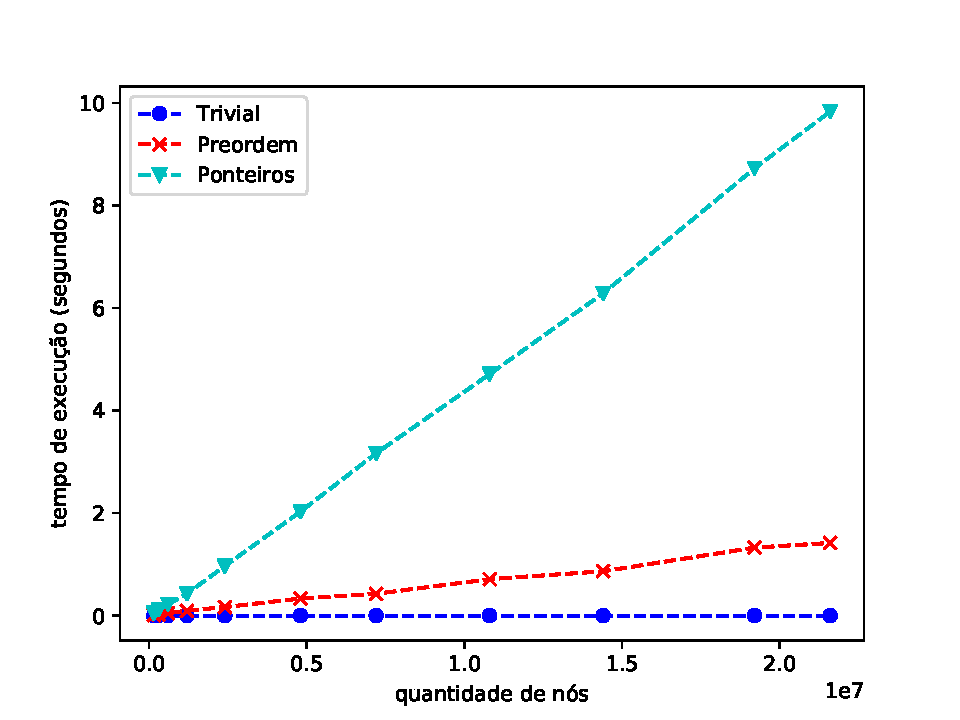
\includegraphics[scale=0.8]{preprocess_linear.pdf}
  \caption{Resultados para o preprocessamento de árvores lineares.}
\end{figure}

\newpage

\subsubsection{Árvores binárias}
Para estas árvores já é possível rodar o Algoritmo da Tabela para todos os tamanhos já
que sua complexidade de espaço agora é $\bigO(n \log n)$, sendo comparável com o
Algoritmo dos Ponteiros, que se mostrou menos eficiente. O Algoritmo da Preordem se tornou
ainda mais rápido, provavelmente por serem necessárias menos alocações de memória.

\begin{figure}
  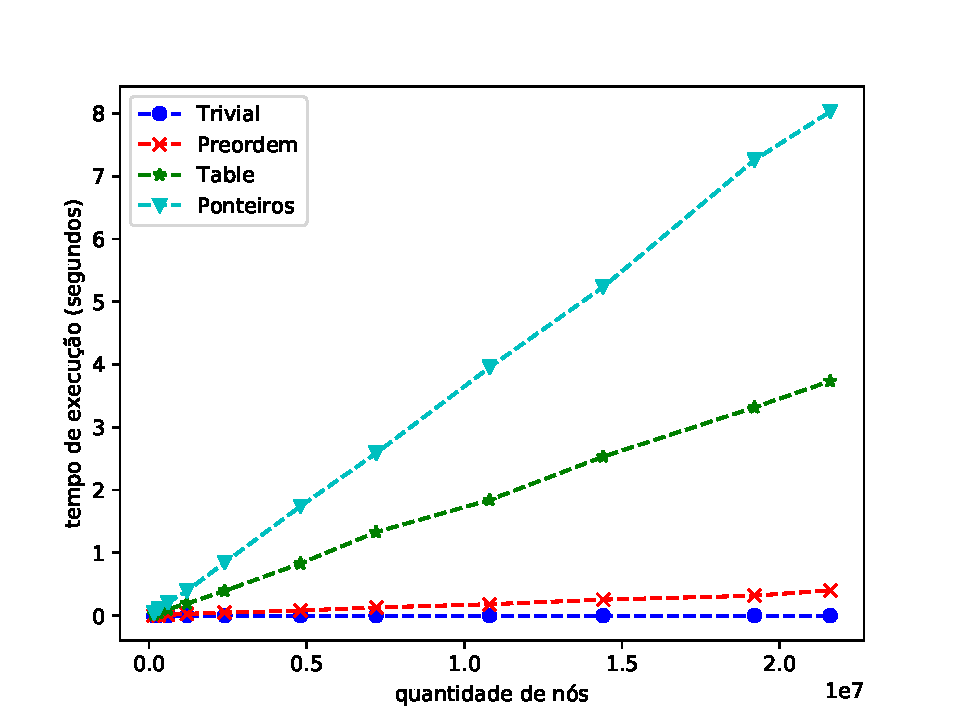
\includegraphics[scale=0.8]{preprocess_binary.pdf}
  \caption{Resultados para o preprocessamento de árvores binárias.}
\end{figure}

\subsubsection{Árvores quaternárias}
Para estas árvores é interessante notar que o desempenho do Algoritmo da Tabela foi
maior do que para árvores binárias e isso se deve à relação entre sua complexidade
de tempo e o fator de ramificação da árvore, já que esta é $\bigO(n \log_k n)$, onde
$k$ é o fator. O Algoritmo dos Ponteiros se manteve estável já que sua complexidade
não depende de $k$.

\begin{figure}[H]
  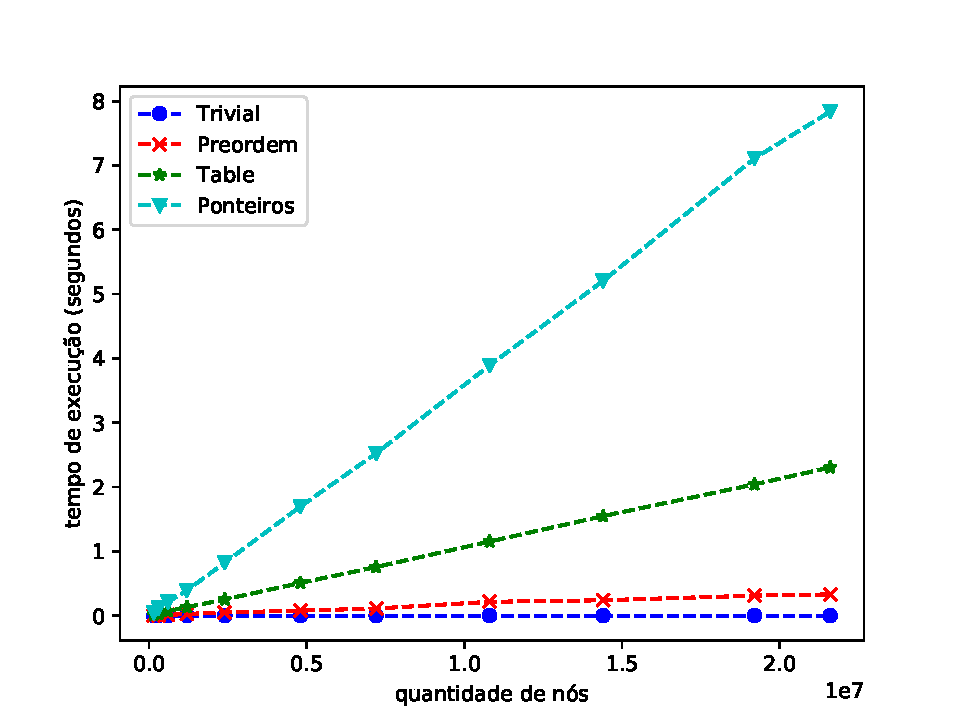
\includegraphics[scale=0.8]{preprocess_4ary.pdf}
  \caption{Resultados para o preprocessamento de árvores quaternárias.}
\end{figure}

\subsection{Consultas}

\subsubsection{Árvores lineares}
\subsubsection{Árvores binárias}

\begin{figure}[H]
  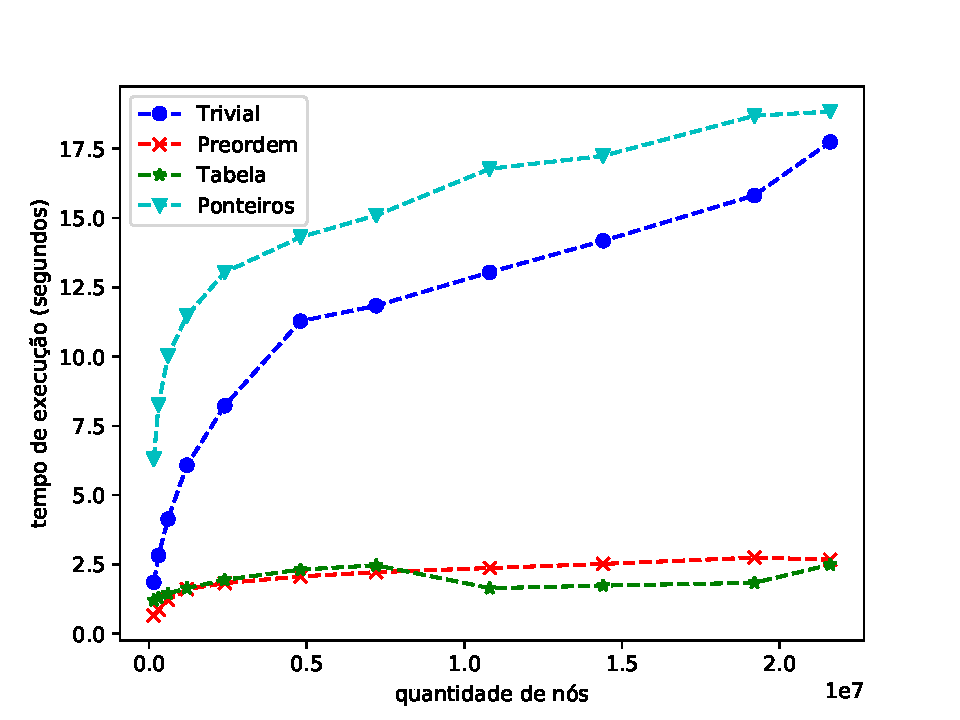
\includegraphics[scale=0.8]{query_binary.pdf}
  \caption{Resultados para as consultas em árvores binárias.}
\end{figure}

\subsubsection{Árvores quaternárias}

\begin{figure}[H]
  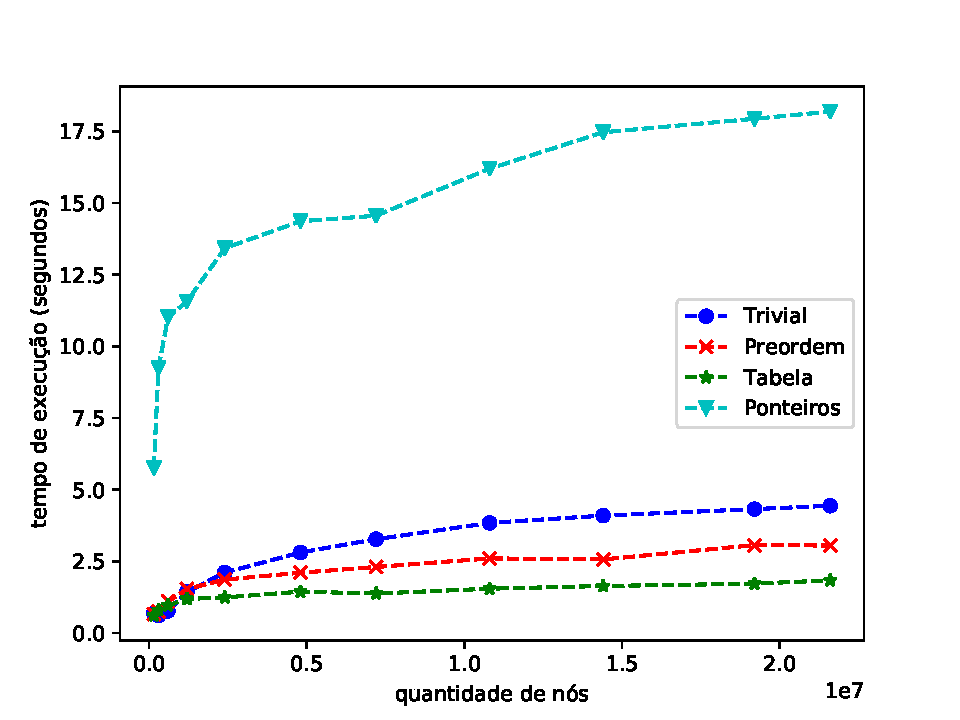
\includegraphics[scale=0.8]{query_4ary.pdf}
  \caption{Resultados para as consultas em árvores quaternárias.}
\end{figure}

\subsection{Conclusões}
Quase todos os algoritmos, exceto pelo algoritmo dos Ponteiros, se mostram mais
eficientes à medida que o fator de ramificação da árvore aumenta, já que isso causa
uma diminuição na sua profundidade esperada, que por sua vez tem relação direta com
a complexidade das implementações. É bastante interessante notar que implementações
simples como o algoritmo da Preordem e o da Tabela podem obter resultados muito
melhores do que outros mais complexos como o algoritmo dos Ponteiros. 
\par

\par


%%%%%%%%%%%%%%%%%%%%%%%%%%%% APÊNDICES E ANEXOS %%%%%%%%%%%%%%%%%%%%%%%%%%%%%%%%

% Um apêndice é algum conteúdo adicional de sua autoria que colabora com a
% ideia geral do texto mas que, por alguma razão, não precisa fazer parte
% da sequência do discurso; por exemplo, a demonstração de um teorema, as
% perguntas usadas em uma pesquisa qualitativa etc.
%
% Um anexo é um documento que não é de sua autoria mas que é relevante para
% a tese; por exemplo, a especificação do padrão que o trabalho discute.
%
% Os comandos appendix e annex reiniciam a numeração de capítulos e passam
% a numerá-los com letras. "annex" não faz parte de nenhuma classe padrão,
% ele foi criado para este modelo (em annex.sty e utils.tex). Se o
% trabalho não tiver apêndices ou anexos, remova estas linhas.
%
% Diferentemente de \mainmatter, \backmatter etc., \appendix e \annex não
% forçam o início de uma nova página. Em geral isso não é importante, pois
% o comando seguinte costuma ser "\chapter", mas pode causar problemas com
% a formatação dos cabeçalhos. Assim, vamos forçar uma nova página antes
% de cada um deles.

%%%% Apêndices %%%%
%\makeatletter
%\if@openright\cleardoublepage\else\clearpage\fi
%\makeatother

% Este formato está definido na package imeusp-headers.
%\pagestyle{appendix}

%\appendix

%%!TeX root=../tese.tex
%("dica" para o editor de texto: este arquivo é parte de um documento maior)
% para saber mais: https://tex.stackexchange.com/q/78101/183146

% Os apêndices podem ser inseridos diretamente aqui ou "puxados" de outros
% arquivos
%!TeX root=../tese.tex
%("dica" para o editor de texto: este arquivo é parte de um documento maior)
% para saber mais: https://tex.stackexchange.com/q/78101/183146

\chapter{Testes de unidade com a biblioteca Catch2}
\label{ap:pseudocode}

Para garantir a corretude dos algoritmos implementados neste trabalho, já estava
decidido desde o início a utilizar alguma ferramenta para realizar testes que pudessem
facilmente identificar erros nas implementações ao longo do ano. Depois de pesquisar
bastante optei por utilizar a biblioteca \textbf{Catch2} por ser \textit{header-only}
e facilitar o processo de rodar em outras máquinas sem precisar instalar nada.
A sintaxe do \textit{framework} fornecido pela biblioteca é bem organizada e foi
de fácil utilização. No programa ~\ref{prog:tabletest} consta uma parte do código
real dos testes do Algoritmo da Tabela, exemplificando quão simples é escrever testes
de unidade bem separados por classe e tipo de teste, podendo criar diversos casos de
teste, cada um com um \textit{setup} diferente de variáveis e objetos.

Para este estudo, cada algoritmo teve seus testes encapsulados dentro de casos de teste
(\texttt{TEST\_CASE}) enquanto cada tipo de teste dentro de cada algoritmo (árvores lineares, binárias
e quaternárias) foram colocados dentro de suas próprias seções (\texttt{SECTION}). As asserções, que
fazem o papel de garantir que algo realmente vale é feito através das macros
\texttt{REQUIRE}, que checa igualdade entre dois valores e \texttt{REQUIRE\_THROW\_AS},
que verifica se uma função levantou a exceção que era esperada.

\begin{program}[H]
      \lstinputlisting[
        language=c++,
        style=pseudocode,
        style=wider,
        functions={TableAlgorithm, build_balanced_kary_tree, Tree},
        specialidentifiers={TEST_CASE, SECTION, REQUIRE, REQUIRE_THROWS_AS},
      ]
      {conteudo-exemplo/catch2-1.cpp}
    
      \caption{Parte dos testes para o Algoritmo da Tabela.\label{prog:tabletest}}
    \end{program}

\par

%%!TeX root=../tese.tex
%("dica" para o editor de texto: este arquivo é parte de um documento maior)
% para saber mais: https://tex.stackexchange.com/q/78101/183146

% Os apêndices podem ser inseridos diretamente aqui ou "puxados" de outros
% arquivos
%!TeX root=../tese.tex
%("dica" para o editor de texto: este arquivo é parte de um documento maior)
% para saber mais: https://tex.stackexchange.com/q/78101/183146

\chapter{Testes de unidade com a biblioteca Catch2}
\label{ap:pseudocode}

Para garantir a corretude dos algoritmos implementados neste trabalho, já estava
decidido desde o início a utilizar alguma ferramenta para realizar testes que pudessem
facilmente identificar erros nas implementações ao longo do ano. Depois de pesquisar
bastante optei por utilizar a biblioteca \textbf{Catch2} por ser \textit{header-only}
e facilitar o processo de rodar em outras máquinas sem precisar instalar nada.
A sintaxe do \textit{framework} fornecido pela biblioteca é bem organizada e foi
de fácil utilização. No programa ~\ref{prog:tabletest} consta uma parte do código
real dos testes do Algoritmo da Tabela, exemplificando quão simples é escrever testes
de unidade bem separados por classe e tipo de teste, podendo criar diversos casos de
teste, cada um com um \textit{setup} diferente de variáveis e objetos.

Para este estudo, cada algoritmo teve seus testes encapsulados dentro de casos de teste
(\texttt{TEST\_CASE}) enquanto cada tipo de teste dentro de cada algoritmo (árvores lineares, binárias
e quaternárias) foram colocados dentro de suas próprias seções (\texttt{SECTION}). As asserções, que
fazem o papel de garantir que algo realmente vale é feito através das macros
\texttt{REQUIRE}, que checa igualdade entre dois valores e \texttt{REQUIRE\_THROW\_AS},
que verifica se uma função levantou a exceção que era esperada.

\begin{program}[H]
      \lstinputlisting[
        language=c++,
        style=pseudocode,
        style=wider,
        functions={TableAlgorithm, build_balanced_kary_tree, Tree},
        specialidentifiers={TEST_CASE, SECTION, REQUIRE, REQUIRE_THROWS_AS},
      ]
      {conteudo-exemplo/catch2-1.cpp}
    
      \caption{Parte dos testes para o Algoritmo da Tabela.\label{prog:tabletest}}
    \end{program}

\par

%\par

%%%% Anexos %%%%
% \makeatletter
% \if@openright\cleardoublepage\else\clearpage\fi
% \makeatother

% Este formato está definido na package imeusp-headers (note que é o mesmo
% que o anterior; repetimos aqui caso você queira desabilitar toda a seção
% de apêndices).
%\pagestyle{appendix}

%\annex

%%!TeX root=../tese.tex
%("dica" para o editor de texto: este arquivo é parte de um documento maior)
% para saber mais: https://tex.stackexchange.com/q/78101/183146

% Os anexos podem ser inseridos diretamente aqui ou "puxados" de outros
% arquivos
%!TeX root=../tese.tex
%("dica" para o editor de texto: este arquivo é parte de um documento maior)
% para saber mais: https://tex.stackexchange.com/q/78101/183146

\chapter[Perguntas Frequentes sobre o Modelo]{Perguntas Frequentes sobre o Modelo\footnote{Esta
seção não é de fato um anexo, mas sim um apêndice; ela foi definida desta
forma apenas para servir como exemplo de anexo.}}

\begin{itemize}

\item \textbf{Posso usar pacotes \LaTeX{} adicionais aos sugeridos?}\\
Com certeza! Você pode modificar o arquivo o quanto desejar, o modelo serve só como uma ajuda inicial para o seu trabalho. Observe, no entanto, que ele é baseado na classe \textsf{book} e deve funcionar, com alterações mínimas, com \textsf{article}; já as classes \textsf{KOMA-Script} ou a classe \textsf{memoir} podem ser mais difíceis de adaptar. Além disso, \textsf{pstricks} e \textit{packages} derivadas dependem da linguagem PostScript e, portanto, não funcionam facilmente com as versões modernas de \LaTeX{}.

\item \textbf{As figuras podem ser colocadas no meio do texto ou devem ficar no final dos capítulos?}\\
Em geral, as figuras devem ser apresentadas assim que forem referenciadas. Colocá-las no final dos capítulos dificultaria um pouco a leitura, mas isso depende do estilo do autor, orientador ou lugar de publicação. Converse com seu orientador!

\item \textbf{As figuras e tabelas são colocadas em lugares ruins.}\\
Veja a discussão a respeito na Seção~\ref{sec:limitations}.

\item \textbf{Estou tendo problemas com caracteres acentuados!}\\
Veja a discussão a respeito na Seção~\ref{sec:limitations}.

\item \textbf{Existe algo específico para citações de páginas web?}\\
Biblatex define o tipo ``online'', que deve ser usado para materiais com título, autor etc., como uma postagem ou comentário em um blog, um gráfico ou mesmo uma mensagem de email para uma lista de discussão. Bibtex\index{bibtex}, por padrão, não tem um tipo específico para isso; com ele, normalmente usa-se o campo ``howpublished'' para especificar que se trata de um recurso \textit{online}. Se o que você está citando não é algo determinado com título, autor etc. mas sim um sítio (como uma empresa ou um produto), pode ser mais adequado colocar a referência apenas como nota de rodapé e não na lista de referências; nesses casos, algumas pessoas acrescentam uma segunda lista de referências especificamente para recursos \textit{online} (biblatex\index{biblatex} permite criar múltiplas bibliografias). Já artigos disponíveis \textit{online} mas que fazem parte de uma publicação de formato tradicional (mesmo que apenas \textit{online}), como os anais de um congresso, devem ser citados por seu tipo verdadeiro e apenas incluir o campo ``url'' (não é nem necessário usar o comando \textsf{\textbackslash{}url\{\}}), aceito por todos os tipos de documento do bibtex/biblatex.

\item \textbf{A bibliografia está sendo impressa em inglês (usa ``and'' ao invés de ``e'' para separar os nomes dos autores).}\\
Você deve estar usando um estilo de bibliografia bibtex diferente dos sugeridos. Uma simples solução é copiar o arquivo de estilo correspondente da sua instalação \LaTeX{} para o diretório onde seus arquivos estão e mudar ``and'' por ``e'' (ou ``\&'' se preferir) na função format.names. O mais recomendado, no entanto, é usar biblatex: ele é mais fácil de adaptar para diferentes estilos, tem pleno suporte a diferentes línguas e é possível personalizar as traduções (há um exemplo no modelo).

\item \textbf{Aparece uma folha em branco entre os capítulos}\\
Essa característica foi colocada propositalmente, dado que todo capítulo deve (ou deveria) começar em uma página de numeração ímpar (lado direito do documento). Se quiser mudar esse comportamento, acrescente ``openany'' como opção da classe, i.e., \textsf{\textbackslash{}documentclass[openany,11pt,twoside,a4paper]\{book\}}.

\item \textbf{É possível resumir o nome das seções/capítulos que aparece no topo das páginas e no sumário?}\\
Sim, usando a sintaxe \textsf{\textbackslash{}section[mini-titulo]\{titulo enorme\}}. Isso é especialmente útil nos \textit{captions}\index{Legendas} das figuras e tabelas, que muitas vezes são demasiadamente longos para a lista de figuras/tabelas.

\item \textbf{Existe algum programa para gerenciar referências em formato bibtex?}\\
Sim, há vários. Uma opção bem comum é o JabRef; outra é usar Zotero\index{Zotero} ou Mendeley\index{Mendeley} e exportar os dados deles no formato .bib.

\item \textbf{Como faço para usar o Makefile (comando make) no Windows?}\\
Lembre-se que a ferramenta recomendada para compilação do documento é o \textsf{latexmk}, então você não precisa do \textsf{make}. Mas, se quiser usá-lo, você pode instalar o MSYS2 (\url{www.msys2.org}) ou o Windows Subsystem for Linux (procure as versões de Linux disponíveis na Microsoft Store). Se você pretende usar algum dos editores sugeridos, é possível deixar a compilação a cargo deles, também dispensando o \textsf{make}.

\item \textbf{Como eu faço para...}\\
Leia os comentários dos arquivos ``tese.tex'' e outros que compõem este modelo, além do tutorial (Capítulo \ref{chap:tutorial}) e dos exemplos do Capítulo \ref{chap:exemplos}; é provável que haja uma dica neles ou, pelo menos, a indicação da \textit{package} relacionada ao que você precisa.

\end{itemize}

\par

%%!TeX root=../tese.tex
%("dica" para o editor de texto: este arquivo é parte de um documento maior)
% para saber mais: https://tex.stackexchange.com/q/78101/183146

% Os anexos podem ser inseridos diretamente aqui ou "puxados" de outros
% arquivos
%!TeX root=../tese.tex
%("dica" para o editor de texto: este arquivo é parte de um documento maior)
% para saber mais: https://tex.stackexchange.com/q/78101/183146

\chapter[Perguntas Frequentes sobre o Modelo]{Perguntas Frequentes sobre o Modelo\footnote{Esta
seção não é de fato um anexo, mas sim um apêndice; ela foi definida desta
forma apenas para servir como exemplo de anexo.}}

\begin{itemize}

\item \textbf{Posso usar pacotes \LaTeX{} adicionais aos sugeridos?}\\
Com certeza! Você pode modificar o arquivo o quanto desejar, o modelo serve só como uma ajuda inicial para o seu trabalho. Observe, no entanto, que ele é baseado na classe \textsf{book} e deve funcionar, com alterações mínimas, com \textsf{article}; já as classes \textsf{KOMA-Script} ou a classe \textsf{memoir} podem ser mais difíceis de adaptar. Além disso, \textsf{pstricks} e \textit{packages} derivadas dependem da linguagem PostScript e, portanto, não funcionam facilmente com as versões modernas de \LaTeX{}.

\item \textbf{As figuras podem ser colocadas no meio do texto ou devem ficar no final dos capítulos?}\\
Em geral, as figuras devem ser apresentadas assim que forem referenciadas. Colocá-las no final dos capítulos dificultaria um pouco a leitura, mas isso depende do estilo do autor, orientador ou lugar de publicação. Converse com seu orientador!

\item \textbf{As figuras e tabelas são colocadas em lugares ruins.}\\
Veja a discussão a respeito na Seção~\ref{sec:limitations}.

\item \textbf{Estou tendo problemas com caracteres acentuados!}\\
Veja a discussão a respeito na Seção~\ref{sec:limitations}.

\item \textbf{Existe algo específico para citações de páginas web?}\\
Biblatex define o tipo ``online'', que deve ser usado para materiais com título, autor etc., como uma postagem ou comentário em um blog, um gráfico ou mesmo uma mensagem de email para uma lista de discussão. Bibtex\index{bibtex}, por padrão, não tem um tipo específico para isso; com ele, normalmente usa-se o campo ``howpublished'' para especificar que se trata de um recurso \textit{online}. Se o que você está citando não é algo determinado com título, autor etc. mas sim um sítio (como uma empresa ou um produto), pode ser mais adequado colocar a referência apenas como nota de rodapé e não na lista de referências; nesses casos, algumas pessoas acrescentam uma segunda lista de referências especificamente para recursos \textit{online} (biblatex\index{biblatex} permite criar múltiplas bibliografias). Já artigos disponíveis \textit{online} mas que fazem parte de uma publicação de formato tradicional (mesmo que apenas \textit{online}), como os anais de um congresso, devem ser citados por seu tipo verdadeiro e apenas incluir o campo ``url'' (não é nem necessário usar o comando \textsf{\textbackslash{}url\{\}}), aceito por todos os tipos de documento do bibtex/biblatex.

\item \textbf{A bibliografia está sendo impressa em inglês (usa ``and'' ao invés de ``e'' para separar os nomes dos autores).}\\
Você deve estar usando um estilo de bibliografia bibtex diferente dos sugeridos. Uma simples solução é copiar o arquivo de estilo correspondente da sua instalação \LaTeX{} para o diretório onde seus arquivos estão e mudar ``and'' por ``e'' (ou ``\&'' se preferir) na função format.names. O mais recomendado, no entanto, é usar biblatex: ele é mais fácil de adaptar para diferentes estilos, tem pleno suporte a diferentes línguas e é possível personalizar as traduções (há um exemplo no modelo).

\item \textbf{Aparece uma folha em branco entre os capítulos}\\
Essa característica foi colocada propositalmente, dado que todo capítulo deve (ou deveria) começar em uma página de numeração ímpar (lado direito do documento). Se quiser mudar esse comportamento, acrescente ``openany'' como opção da classe, i.e., \textsf{\textbackslash{}documentclass[openany,11pt,twoside,a4paper]\{book\}}.

\item \textbf{É possível resumir o nome das seções/capítulos que aparece no topo das páginas e no sumário?}\\
Sim, usando a sintaxe \textsf{\textbackslash{}section[mini-titulo]\{titulo enorme\}}. Isso é especialmente útil nos \textit{captions}\index{Legendas} das figuras e tabelas, que muitas vezes são demasiadamente longos para a lista de figuras/tabelas.

\item \textbf{Existe algum programa para gerenciar referências em formato bibtex?}\\
Sim, há vários. Uma opção bem comum é o JabRef; outra é usar Zotero\index{Zotero} ou Mendeley\index{Mendeley} e exportar os dados deles no formato .bib.

\item \textbf{Como faço para usar o Makefile (comando make) no Windows?}\\
Lembre-se que a ferramenta recomendada para compilação do documento é o \textsf{latexmk}, então você não precisa do \textsf{make}. Mas, se quiser usá-lo, você pode instalar o MSYS2 (\url{www.msys2.org}) ou o Windows Subsystem for Linux (procure as versões de Linux disponíveis na Microsoft Store). Se você pretende usar algum dos editores sugeridos, é possível deixar a compilação a cargo deles, também dispensando o \textsf{make}.

\item \textbf{Como eu faço para...}\\
Leia os comentários dos arquivos ``tese.tex'' e outros que compõem este modelo, além do tutorial (Capítulo \ref{chap:tutorial}) e dos exemplos do Capítulo \ref{chap:exemplos}; é provável que haja uma dica neles ou, pelo menos, a indicação da \textit{package} relacionada ao que você precisa.

\end{itemize}

\par

%\par


%%%%%%%%%%%%%%%%%%%%%%%%%%%%%% SEÇÕES FINAIS %%%%%%%%%%%%%%%%%%%%%%%%%%%%%%%%%%%

% Aqui vão a bibliografia, índice remissivo e outras seções similares.

% O comando backmatter desabilita a numeração de capítulos.
\backmatter

% Este formato está definido na package imeusp-headers
\pagestyle{backmatter}

% Espaço adicional no sumário antes das referências / índice remissivo
\addtocontents{toc}{\vspace{2\baselineskip plus .5\baselineskip minus .5\baselineskip}}

% A bibliografia é obrigatória

%%%%%%%%% Bibliografia com natbib (preterido): %%%%%%%%%
%\bibliographystyle{extras/alpha-ime}% citação bibliográfica alpha
%\bibliographystyle{extras/plainnat-ime} % citação bibliográfica textual
%\bibliography{bibliografia}  % associado ao arquivo: 'bibliografia.bib'

%%%%%%%% Bibliografia com biblatex (preferido): %%%%%%%%

\printbibliography[
  title=\refname\label{bibliografia}, % "Referências", recomendado pela ABNT
  %title=\bibname\label{bibliografia}, % "Bibliografia"
  % Inclui a bibliografia no sumário
  heading=bibintoc,
]

% imprime o índice remissivo no documento (opcional)
\printindex

\end{document}
